% ============================================================
%  يُترجَم بـ XeLaTeX  (في Overleaf: Menu → Compiler → XeLaTeX)
%  الخط: Amiri (متوفر في Overleaf، أو حمّله من github.com/aliftype/amiri)
% ============================================================
\documentclass[12pt,a4paper]{article}
\usepackage[a4paper,margin=1.7cm,top=2.3cm,bottom=2.9cm,headheight=15pt,footskip=1.5cm]{geometry}
\usepackage{amsmath,amssymb}
\usepackage{icomma}
\usepackage[english,bidi=default,layout=lists]{babel}
\babelprovide[import,main]{arabic}
\babelfont{rm}[Scale=1.08]{Amiri}
\babelfont{sf}[Scale=1.08]{Amiri}
\usepackage[most]{tcolorbox}
\usepackage{tikz}
\usetikzlibrary{arrows.meta,calc,shadings}
\usepackage{array}
\usepackage{colortbl}
\usepackage{fancyhdr}
\usepackage{titlesec}
\usepackage{enumitem}
\usepackage{collcell}
\usepackage{needspace}
\usepackage{etoolbox}
\newcolumntype{C}{>{\collectcell\ar}c<{\endcollectcell}}
\pretocmd{\section}{\Needspace{15\baselineskip}}{}{}
\pretocmd{\subsection}{\Needspace{11\baselineskip}}{}{}

\definecolor{cDef}{HTML}{1F4E9C}
\definecolor{cThm}{HTML}{B3261E}
\definecolor{cRem}{HTML}{2E7D32}
\definecolor{cEx}{HTML}{C76B00}
\definecolor{cMeth}{HTML}{6A1B9A}
\definecolor{cSol}{HTML}{00695C}
\definecolor{cSec}{HTML}{1F3A68}

\titleformat{\section}{\Large\bfseries\color{cSec}}{\thesection.}{0.6em}{}[{\color{cSec!60}\titlerule[1pt]}]
\titleformat{\subsection}{\large\bfseries\color{cThm!85!black}}{\thesubsection.}{0.5em}{}
\titlespacing*{\section}{0pt}{14pt}{8pt}
\titlespacing*{\subsection}{0pt}{10pt}{5pt}
\setlength{\parindent}{0pt}
\setlength{\parskip}{4pt}
\setlist{itemsep=2pt,topsep=3pt}

\newtcolorbox{arbox}[3][]{enhanced,
  colback=#2!5,colframe=#2!80!black,arc=2mm,boxrule=0.8pt,
  left=6pt,right=6pt,top=8pt,bottom=5pt,
  fonttitle=\bfseries,coltitle=white,
  title={\foreignlanguage{arabic}{#3}},
  attach boxed title to top right={xshift=-5mm,yshift=-3mm},
  boxed title style={colback=#2!80!black,arc=1.5mm,boxrule=0pt},
  before upper={\selectlanguage{arabic}},
  before skip=8pt,after skip=8pt,breakable,#1}
\newenvironment{BOX}[2]{\begin{otherlanguage}{english}\begin{arbox}{#1}{#2}}{\end{arbox}\end{otherlanguage}}
\newenvironment{tarif}[1][تعريف]{\begin{BOX}{cDef}{#1}}{\end{BOX}}
\newenvironment{khassia}[1][خاصية]{\begin{BOX}{cThm}{#1}}{\end{BOX}}
\newenvironment{molahada}[1][ملاحظة]{\begin{BOX}{cRem}{#1}}{\end{BOX}}
\newenvironment{mithal}[1][مثال]{\begin{BOX}{cEx}{#1}}{\end{BOX}}
\newenvironment{tariqa}[1][طريقة]{\begin{BOX}{cMeth}{#1}}{\end{BOX}}

\newcounter{exo}
\newenvironment{tamrin}[1]{\stepcounter{exo}\begin{BOX}{cSec}{التمرين \theexo: #1}}{\end{BOX}}
\newenvironment{hal}{\Needspace{12\baselineskip}\begin{otherlanguage}{english}\begin{arbox}[breakable]{cSol}{حل التمرين \theexo}}{\end{arbox}\end{otherlanguage}}

\newenvironment{LTR}{\begin{otherlanguage}{english}}{\end{otherlanguage}}
\newcommand{\ar}[1]{\foreignlanguage{arabic}{#1}}

\renewcommand{\dots}{\mathinner{\ldotp\ldotp\ldotp}}
\renewcommand{\ldots}{\mathinner{\ldotp\ldotp\ldotp}}
\renewcommand{\cdots}{\mathinner{\cdotp\cdotp\cdotp}}
\newcommand{\N}{\mathbb{N}}
\newcommand{\Z}{\mathbb{Z}}
\newcommand{\D}{\mathbb{D}}
\newcommand{\Q}{\mathbb{Q}}
\newcommand{\R}{\mathbb{R}}
\newcommand{\pgcd}{\operatorname{PGCD}}
\newcommand{\ppcm}{\operatorname{PPCM}}

% \NLseg{a}{b}{[}{]} ; \NLright{a}{[} ; \NLleft{b}{]}  (interval on a number line)
\newcommand{\NLseg}[4]{\begin{LTR}\begin{tikzpicture}[baseline=-0.6ex]
 \draw[-{Stealth[length=2mm]},gray!70](0,0)--(3.4,0);
 \draw[line width=2pt,cThm!80!black](0.7,0)--(2.7,0);
 \node[cThm!80!black,font=\LARGE] at (0.7,0){$#3$};
 \node[cThm!80!black,font=\LARGE] at (2.7,0){$#4$};
 \node[below=3pt,font=\footnotesize] at (0.7,0){$#1$};
 \node[below=3pt,font=\footnotesize] at (2.7,0){$#2$};
\end{tikzpicture}\end{LTR}}
\newcommand{\NLright}[2]{\begin{LTR}\begin{tikzpicture}[baseline=-0.6ex]
 \draw[-{Stealth[length=2mm]},gray!70](0,0)--(3.4,0);
 \draw[line width=2pt,cThm!80!black](1.3,0)--(3.3,0);
 \node[cThm!80!black,font=\LARGE] at (1.3,0){$#2$};
 \node[below=3pt,font=\footnotesize] at (1.3,0){$#1$};
\end{tikzpicture}\end{LTR}}
\newcommand{\NLleft}[2]{\begin{LTR}\begin{tikzpicture}[baseline=-0.6ex]
 \draw[-{Stealth[length=2mm]},gray!70](0,0)--(3.4,0);
 \draw[line width=2pt,cThm!80!black](0.05,0)--(2.1,0);
 \node[cThm!80!black,font=\LARGE] at (2.1,0){$#2$};
 \node[below=3pt,font=\footnotesize] at (2.1,0){$#1$};
\end{tikzpicture}\end{LTR}}

% ---------- social-media icons (pure TikZ) ----------
\definecolor{cFB}{HTML}{1877F2}
\definecolor{cTG}{HTML}{229ED9}
\definecolor{cIG1}{HTML}{FEDA75}
\definecolor{cIG2}{HTML}{D62976}
\definecolor{cIG3}{HTML}{4F5BD5}
\newcommand{\fbicon}{\begin{LTR}\begin{tikzpicture}[baseline=-0.75ex,x=1em,y=1em]
 \fill[cFB] (0,0) circle (0.55);
 \node[white,inner sep=0,font=\usefont{TU}{lmss}{bx}{n}\small] at (0.04,-0.02) {f};
\end{tikzpicture}\end{LTR}}
\newcommand{\igicon}{\begin{LTR}
\begin{tikzpicture}[baseline=-0.75ex,x=1em,y=1em]
 \shade[lower left=cIG1,lower right=cIG2,upper left=cIG2,upper right=cIG3,rounded corners=0.28em] (-0.55,-0.55) rectangle (0.55,0.55);
 \draw[white,line width=0.09em,rounded corners=0.18em] (-0.36,-0.36) rectangle (0.36,0.36);
 \draw[white,line width=0.09em] (0,0) circle (0.17);
 \fill[white] (0.22,0.22) circle (0.05);
\end{tikzpicture}\end{LTR}}
\newcommand{\tgicon}{\begin{LTR}
\begin{tikzpicture}[baseline=-0.75ex,x=1em,y=1em]
 \fill[cTG] (0,0) circle (0.55);
 \fill[white] (-0.33,0.0) -- (0.32,0.27) -- (0.2,-0.3) -- (0.0,-0.15) -- (-0.08,-0.28) -- (-0.08,-0.08) -- cycle;
 \fill[cTG!70!black] (-0.08,-0.08) -- (0.25,0.2) -- (0.0,-0.15) -- (-0.08,-0.28) -- cycle;
\end{tikzpicture}\end{LTR}}
% page number: black box, white two-digit number, at the right of the social row
\newcommand{\PageBox}{\begin{LTR}\tikz[baseline=(p.base)]\node[fill=black,text=white,inner sep=2.5pt,minimum width=1.6em,minimum height=1.3em,font=\usefont{TU}{lmss}{bx}{n}\small](p){\ifnum\value{page}<10 0\fi\arabic{page}};\end{LTR}}
% visual left-to-right order: Telegram | Instagram | Facebook | page box
\newcommand{\SocialRow}{\begin{otherlanguage}{english}%
 \ar{\textbf{الأستاذ سوايسية هشام للرياضيات}}\ \tgicon\hfill
 \textbf{prof\_hicham\_math}\ \igicon\hfill
 \ar{\textbf{الأستاذ سوايسية هشام للرياضيات}}\ \fbicon\hspace{2.2em}\PageBox\end{otherlanguage}}

\pagestyle{fancy}
\fancyhf{}
\renewcommand{\headrulewidth}{0.6pt}
\renewcommand{\footrulewidth}{0.4pt}
% \SetHeader{right head: document title}{left head: level -- stream}
\newcommand{\SetHeader}[2]{%
 \fancyhead[C]{\parbox{\textwidth}{\ar{#1\hfill #2}}}%
 \fancyfoot[C]{\parbox{\textwidth}{\small\SocialRow}}}
\usepackage{tkz-tab}
\usepackage{multicol}
% variation / sign table (LTR)
\newenvironment{TAB}{\par\begin{center}\begin{LTR}\begin{tikzpicture}[scale=0.95,every node/.style={font=\small}]}{\end{tikzpicture}\end{LTR}\end{center}}
% grid + axes, clipped: \begin{GR}{xmin}{xmax}{ymin}{ymax}{unit cm}
\newenvironment{GR}[5]{\par\begin{center}\begin{LTR}\begin{tikzpicture}[x=#5cm,y=#5cm,font=\footnotesize]
 \draw[gray!25,very thin] (#1,#3) grid (#2,#4);
 \draw[-{Stealth[length=2mm]}] (#1,0)--(#2+0.3,0) node[below left]{$x$};
 \draw[-{Stealth[length=2mm]}] (0,#3)--(0,#4+0.3) node[below left]{$y$};
 \node[below left] at (0,0){$O$};
 \begin{scope}\clip (#1,#3) rectangle (#2,#4);}
{\end{scope}\end{tikzpicture}\end{LTR}\end{center}}
\newcommand{\Ticks}[2]{\foreach \t in {#1} \node[below,font=\scriptsize] at (\t,0){$\t$}; \foreach \t in {#2} \node[left,font=\scriptsize] at (0,\t){$\t$};}
\newcommand{\bx}[1]{\ensuremath{\colorbox{cDef!12}{$\displaystyle #1$}}}
\newcommand{\TwoCol}[4]{\par\begin{LTR}\noindent\begin{minipage}[t]{#1\textwidth}\selectlanguage{arabic}#2\end{minipage}\hfill\begin{minipage}[t]{#3\textwidth}\selectlanguage{arabic}#4\end{minipage}\end{LTR}\par}
\newcommand{\RL}[4]{\TwoCol{#3}{#4}{#1}{#2}}  % \RL{w1}{right content}{w2}{left content}
\newcommand{\ok}{$\textcolor{cRem}{\checkmark}$}
\newcommand{\limn}{\displaystyle\lim_{n\to+\infty}}
% sub-questions, each on its own line
\newenvironment{sq}{\begin{itemize}[leftmargin=2.4em,itemsep=3pt]}{\end{itemize}}
\newcommand{\qa}{\item[(أ)]}\newcommand{\qb}{\item[(ب)]}\newcommand{\qc}{\item[(جـ)]}\newcommand{\qd}{\item[(د)]}\newcommand{\qe}{\item[(هـ)]}
\newcommand{\pa}{\par\smallskip\textbf{(أ)} }\newcommand{\pb}{\par\smallskip\textbf{(ب)} }\newcommand{\pc}{\par\smallskip\textbf{(جـ)} }\newcommand{\pd}{\par\smallskip\textbf{(د)} }\newcommand{\pe}{\par\smallskip\textbf{(هـ)} }
\newcommand{\QQ}[1]{\par\smallskip\textbf{#1.} }
\newenvironment{tmr}{\stepcounter{exo}\begin{BOX}{cSec}{تمرين محلول \theexo}}{\end{BOX}}
\newcommand{\ABC}[3]{\\[2pt]\begin{tabular}{p{0.28\textwidth}p{0.28\textwidth}p{0.28\textwidth}}(جـ) \ #3 & (ب) \ #2 & (أ) \ #1\end{tabular}}
\pretocmd{\section}{\Needspace{24\baselineskip}}{}{}
\newtcbox{\bxtbox}{on line,colback=cDef!12,colframe=cDef!12,boxrule=0pt,arc=1pt,boxsep=0pt,left=2pt,right=2pt,top=1pt,bottom=1pt}
\newcommand{\bxt}[1]{\foreignlanguage{english}{\bxtbox{\ar{#1}}}}
\SetHeader{\small\bfseries\color{cSec}تمارين البكالوريا: الدوال الأصلية والحساب التكاملي}{\small\color{cSec}السنة الثالثة ثانوي -- الشعب العلمية}
\begin{document}
\begin{LTR}
\begin{tcolorbox}[enhanced,colback=cSec,colframe=cSec,arc=3mm,halign=center,boxrule=0pt,top=12pt,bottom=12pt,before upper={\selectlanguage{arabic}}]
{\color{white}\fontsize{22}{28}\selectfont\bfseries تمارين البكالوريا في الدوال الأصلية والحساب التكاملي}\\[8pt]
{\color{white}\large مع الحلول المفصلة -- حتى دورة 2026}\\[5pt]
{\color{white}\large علوم تجريبية -- تقني رياضي -- رياضيات}
\end{tcolorbox}
\end{LTR}
\section{تمارين البكالوريا -- شعبة علوم تجريبية}
% ===================== 2026 -- 1 =====================
\begin{tamrin}{بكالوريا 2026 -- الموضوع الأول -- علوم تجريبية}
$f$ الدالة المعرفة على $[0;+\infty[$ بـ: $f(x)=x^2+2x-4x\ln x$ من أجل كل $x>0$ و $f(0)=0$.
$(C_f)$ تمثيلها البياني في المستوي المنسوب إلى المعلم المتعامد والمتجانس $(O;\vec i,\vec j)$.
\QQ{1}
\begin{sq}
\qa باستعمال المكاملة بالتجزئة، بيّن أن: $\displaystyle\int_1^e x\ln x\,dx=\frac{e^2+1}{4}$.
\qb أحسب $\mathcal{A}$ مساحة الحيز المستوي المحدد بـ $(C_f)$ والمستقيمات التي معادلاتها: $y=0$، $x=1$ و $x=e$.
\end{sq}
\end{tamrin}

\begin{hal}
\QQ{1}
\pa \textbf{المكاملة بالتجزئة:} نضع من أجل كل $x\in[1;e]$:
\[u(x)=\ln x\ \Rightarrow\ u'(x)=\frac1x\qquad;\qquad v'(x)=x\ \Rightarrow\ v(x)=\frac{x^2}{2}\]
الدالتان $u$ و $v$ قابلتان للاشتقاق على $[1;e]$ ومشتقتاهما مستمرتان عليه، إذن:
\[\int_1^e x\ln x\,dx=\Big[\frac{x^2}{2}\ln x\Big]_1^e-\int_1^e\frac{x^2}{2}\cdot\frac1x\,dx=\Big(\frac{e^2}{2}\ln e-\frac12\ln 1\Big)-\int_1^e\frac{x}{2}\,dx\]
\[=\frac{e^2}{2}-\Big[\frac{x^2}{4}\Big]_1^e=\frac{e^2}{2}-\frac{e^2}{4}+\frac14\]
ومنه: \bx{\int_1^e x\ln x\,dx=\frac{e^2+1}{4}}.

\pb \textbf{إشارة $f(x)$ على $[1;e]$:} من أجل $x>0$: $f(x)=x\,\varphi(x)$ حيث $\varphi(x)=x+2-4\ln x$.

$\varphi'(x)=1-\dfrac4x=\dfrac{x-4}{x}$، ومن أجل $x\in[1;e]$ لدينا $x\le e<4$ إذن $\varphi'(x)<0$، أي $\varphi$ متناقصة تماما على $[1;e]$، ومنه من أجل كل $x\in[1;e]$:
$\varphi(x)\ge\varphi(e)=e+2-4=e-2>0$. وبما أن $x>0$ فإن $f(x)>0$ على $[1;e]$.
\begin{TAB}
\tkzTabInit[lgt=3.2,espcl=5]{$x$ /0.8,$f(x)$ /0.8,\ar{الوضع النسبي} /1}{$1$,$e$}
\tkzTabLine{,+,}
\tkzTabLine{,\hbox{\ar{\footnotesize $(C_f)$ فوق محور الفواصل}},}
\end{TAB}
\textbf{حساب المساحة:} بما أن $f(x)\ge 0$ على $[1;e]$ فإن $|f(x)|=f(x)$، وباستعمال خطية التكامل والسؤال (أ):
\[\mathcal{A}=\int_1^e|f(x)|\,dx=\int_1^e(x^2+2x)\,dx-4\int_1^e x\ln x\,dx=\Big[\frac{x^3}{3}+x^2\Big]_1^e-4\cdot\frac{e^2+1}{4}\]
\[=\Big(\frac{e^3}{3}+e^2\Big)-\Big(\frac13+1\Big)-e^2-1=\frac{e^3}{3}-\frac73\]
\[\bx{\mathcal{A}=\frac{e^3-7}{3}\ \text{u.a}\approx 4{,}36\ \text{u.a}}\]
\begin{GR}{-1}{6}{-1}{5}{0.85}
\fill[cDef!25,domain=1:2.71828,samples=80] (1,0) -- plot(\x,{\x*\x+2*\x-4*\x*ln(\x)}) -- (2.71828,0) -- cycle;
\draw[cDef,thick,domain=0.002:6,samples=150] plot(\x,{\x*\x+2*\x-4*\x*ln(\x)});
\draw[dashed] (1,0)--(1,3) (2.71828,0)--(2.71828,1.95);
\node at (1.85,1.2){$\mathcal{A}$};
\node[cDef] at (5.2,4.4){$(C_f)$};
\Ticks{1,2,4,5}{1,2,3,4}
\node[below,font=\scriptsize] at (2.71828,0){$e$};
\end{GR}
\end{hal}

% ===================== 2026 -- 2 =====================
\begin{tamrin}{بكالوريا 2026 -- الموضوع الثاني -- علوم تجريبية}
$f$ الدالة المعرفة على $\R^*$ بـ: $f(x)=1+\dfrac{5-4e^x}{e^{2x}-1}$.
$(C_f)$ تمثيلها البياني في المستوي المنسوب إلى المعلم المتعامد والمتجانس $(O;\vec i,\vec j)$.
\QQ{1}
\begin{sq}
\qa تحقق أنه: من أجل كل $x$ من $\R^*$، $f(x)=-4+\dfrac12\Big(\dfrac{9e^x}{1+e^x}-\dfrac{e^x}{1-e^x}\Big)$.
\qb أحسب بدلالة $\lambda$ المساحة $A(\lambda)$ للحيز المستوي المحدد بـ $(C_f)$ والمستقيمات التي معادلاتها: $y=-4$، $x=\lambda$ و $x=-\ln 2$ حيث $\lambda<-\ln 2$. ثم أحسب $\lim\limits_{\lambda\to-\infty}A(\lambda)$.
\end{sq}
\end{tamrin}

\begin{hal}
\QQ{1}
\pa من أجل $x\in\R^*$ لدينا $e^x\neq1$. نوحّد المقامات في الطرف الثاني:
\[\frac{9e^x}{1+e^x}-\frac{e^x}{1-e^x}=\frac{9e^x(1-e^x)-e^x(1+e^x)}{(1+e^x)(1-e^x)}=\frac{e^x\,(8-10e^x)}{1-e^{2x}}\]
إذن الطرف الثاني يساوي: $-4+\dfrac{e^x(4-5e^x)}{1-e^{2x}}$.

من جهة أخرى:
\[f(x)+4=5+\frac{5-4e^x}{e^{2x}-1}=\frac{5e^{2x}-5+5-4e^x}{e^{2x}-1}=\frac{e^x(5e^x-4)}{e^{2x}-1}=\frac{e^x(4-5e^x)}{1-e^{2x}}\]
ومنه: \bx{f(x)=-4+\frac12\Big(\frac{9e^x}{1+e^x}-\frac{e^x}{1-e^x}\Big)}.

\pb \textbf{الوضع النسبي على $[\lambda;-\ln2]$:} من أجل $x\le-\ln2$: $0<e^x\le\frac12$، إذن:
$e^x>0$، و $4-5e^x\ge4-\frac52=\frac32>0$، و $1-e^{2x}>0$. ومنه $f(x)-(-4)=\dfrac{e^x(4-5e^x)}{1-e^{2x}}>0$.
\begin{TAB}
\tkzTabInit[lgt=3.2,espcl=5]{$x$ /0.8,$f(x)-(-4)$ /0.8,\ar{الوضع النسبي} /1}{$\lambda$,$-\ln2$}
\tkzTabLine{,+,}
\tkzTabLine{,\hbox{\ar{\footnotesize $(C_f)$ فوق المستقيم $y=-4$}},}
\end{TAB}
إذن: $A(\lambda)=\displaystyle\int_\lambda^{-\ln2}|f(x)+4|\,dx=\int_\lambda^{-\ln2}\big(f(x)+4\big)\,dx=\frac12\int_\lambda^{-\ln2}\Big(9\cdot\frac{e^x}{1+e^x}-\frac{e^x}{1-e^x}\Big)dx$.

\textbf{الدوال الأصلية:} $\dfrac{e^x}{1+e^x}$ من الشكل $\dfrac{u'}{u}$ مع $u(x)=1+e^x>0$، فدالة أصلية لها $\ln(1+e^x)$.
و $-\dfrac{e^x}{1-e^x}$ من الشكل $\dfrac{u'}{u}$ مع $u(x)=1-e^x>0$ على $]-\infty;0[$، فدالة أصلية لها $\ln(1-e^x)$. إذن:
\[A(\lambda)=\frac12\Big[9\ln(1+e^x)+\ln(1-e^x)\Big]_\lambda^{-\ln2}\]
مع $e^{-\ln2}=\frac12$: $9\ln\frac32+\ln\frac12=9\ln3-9\ln2-\ln2=9\ln3-10\ln2$. ومنه:
\[\bx{A(\lambda)=\frac12\Big[9\ln3-10\ln2-9\ln(1+e^\lambda)-\ln(1-e^\lambda)\Big]\ \text{u.a}}\]
\textbf{النهاية:} $\lim\limits_{\lambda\to-\infty}e^\lambda=0$، إذن $\lim\ln(1+e^\lambda)=\ln1=0$ و $\lim\ln(1-e^\lambda)=0$، ومنه:
\[\bx{\lim_{\lambda\to-\infty}A(\lambda)=\frac{9\ln3-10\ln2}{2}\ \text{u.a}\approx1{,}48\ \text{u.a}}\]
\begin{GR}{-5}{3}{-5}{4}{0.75}
\fill[cDef!25,domain=-4:-0.6931,samples=80] (-4,-4) -- plot(\x,{1+(5-4*exp(\x))/(exp(2*\x)-1)}) -- (-0.6931,-4) -- cycle;
\draw[cDef,thick,domain=-5:-0.07,samples=150] plot(\x,{1+(5-4*exp(\x))/(exp(2*\x)-1)});
\draw[cDef,thick,domain=0.06:3,samples=150] plot(\x,{1+(5-4*exp(\x))/(exp(2*\x)-1)});
\draw[cThm,thick] (-5,-4)--(3,-4);
\draw[dashed,gray] (-5,1)--(3,1);
\draw[dashed] (-0.6931,-4)--(-0.6931,-3);
\node at (-2.4,-3.6){$\mathcal{A}(\lambda)$};
\node[cDef] at (1.2,2.6){$(C_f)$};
\node[cThm] at (1.8,-4.4){$y=-4$};
\node[below,font=\scriptsize] at (-4,0){$\lambda$};
\draw[dashed] (-4,0)--(-4,-4);
\node[above,font=\scriptsize] at (-0.6931,0){$-\ln2$};
\Ticks{-3,-2,1,2}{-3,-2,-1,1,2,3}
\end{GR}
\end{hal}

% ===================== 2025 -- 1 =====================
\begin{tamrin}{بكالوريا 2025 -- الموضوع الأول -- علوم تجريبية}
$f$ الدالة المعرفة على $\R$ بـ: $f(x)=e^{2x}-e^x-x-2$.
$(C_f)$ تمثيلها البياني في المستوي المنسوب إلى المعلم المتعامد والمتجانس $(O;\vec i,\vec j)$ (الوحدة $2\,cm$).
\QQ{1} أدرس وضعية المنحنى $(C_f)$ بالنسبة إلى المستقيم $(\Delta)$ ذي المعادلة $y=-x-2$.
\QQ{2} أحسب بالسنتيمتر المربع $A$ مساحة الحيز المستوي المحدد بالمنحنى $(C_f)$ والمستقيمات التي معادلاتها: $y=-x-2$، $x=-1$ و $x=0$.
\end{tamrin}

\begin{hal}
\QQ{1} من أجل كل $x\in\R$: $f(x)-(-x-2)=e^{2x}-e^x=e^x(e^x-1)$.
بما أن $e^x>0$ فإن الإشارة هي إشارة $e^x-1$: $e^x-1<0\Leftrightarrow x<0$ و $e^x-1>0\Leftrightarrow x>0$.
\begin{TAB}
\tkzTabInit[lgt=3.2,espcl=4]{$x$ /0.8,$f(x)-(-x-2)$ /0.8,\ar{الوضع النسبي} /1}{$-\infty$,$0$,$+\infty$}
\tkzTabLine{,-,z,+,}
\tkzTabLine{,\hbox{\ar{\footnotesize $(C_f)$ تحت $(\Delta)$}},t,\hbox{\ar{\footnotesize $(C_f)$ فوق $(\Delta)$}},}
\end{TAB}
\bxt{$(C_f)$ تحت $(\Delta)$ على $]-\infty;0[$، فوقه على $]0;+\infty[$، ويقطعه في $(0;-2)$}

\QQ{2} على $[-1;0]$: $(C_f)$ تحت $(\Delta)$ (حسب الجدول)، إذن $|f(x)-(-x-2)|=(-x-2)-f(x)=e^x-e^{2x}$:
\[A=\int_{-1}^{0}\big(e^x-e^{2x}\big)\,dx\ \text{u.a}=\Big[e^x-\frac{e^{2x}}{2}\Big]_{-1}^{0}=\Big(1-\frac12\Big)-\Big(e^{-1}-\frac{e^{-2}}{2}\Big)=\frac12-\frac1e+\frac1{2e^2}=\frac{(e-1)^2}{2e^2}\ \text{u.a}\]
(دالة أصلية لـ $e^{2x}$ هي $\frac12e^{2x}$ لأنها من الشكل $\frac1a e^{ax}$.)

وحدة المساحة: $1\,\text{u.a}=2\,cm\times2\,cm=4\,cm^2$، ومنه:
\[\bx{A=\frac{(e-1)^2}{2e^2}\ \text{u.a}=\frac{2(e-1)^2}{e^2}\,cm^2\approx0{,}80\,cm^2}\]
\begin{GR}{-3}{1.5}{-3}{2.5}{1.2}
\fill[cDef!25] plot[domain=-1:0,samples=60](\x,{exp(2*\x)-exp(\x)-\x-2}) -- plot[domain=0:-1](\x,{-\x-2}) -- cycle;
\draw[cDef,thick,domain=-3:1.4,samples=150] plot(\x,{exp(2*\x)-exp(\x)-\x-2});
\draw[cThm,thick,domain=-3:1.5] plot(\x,{-\x-2});
\draw[dashed] (-1,0)--(-1,-1.23);
\draw[->] (-1.6,-2.6) node[below,font=\scriptsize]{$A$} -- (-0.5,-1.6);
\node[cDef] at (1.05,1.8){$(C_f)$};
\node[cThm] at (-2.6,1.1){$(\Delta)$};
\Ticks{-2,-1,1}{-2,-1,1,2}
\end{GR}
\end{hal}

% ===================== 2025 -- 2 =====================
\begin{tamrin}{بكالوريا 2025 -- الموضوع الثاني -- علوم تجريبية}
$f$ الدالة المعرفة على $]-4;+\infty[$ بـ: $f(x)=\dfrac{x^2\ln(x+4)}{x+4}$.
$(C_f)$ تمثيلها البياني في المستوي المنسوب إلى المعلم المتعامد والمتجانس $(O;\vec i,\vec j)$.
\QQ{1} $h$ الدالة المعرفة على $]-4;+\infty[$ بـ: $h(x)=\dfrac{(x^2+1)\ln(x+4)}{x+4}$، و $(C_h)$ تمثيلها البياني.
\begin{sq}
\qa بيّن أنه: من أجل كل $x$ من $[-3;0]$، $h(x)-f(x)\ge0$.
\qb أحسب $A$ مساحة الحيز المستوي المحدد بـ $(C_f)$، $(C_h)$ والمستقيمين ذوي المعادلتين: $x=-3$ و $x=0$.
\end{sq}
\end{tamrin}

\begin{hal}
\QQ{1}
\pa من أجل كل $x\in]-4;+\infty[$:
\[h(x)-f(x)=\frac{(x^2+1)\ln(x+4)-x^2\ln(x+4)}{x+4}=\frac{\ln(x+4)}{x+4}\]
من أجل $x\in[-3;0]$: $1\le x+4\le4$، إذن $x+4>0$ و $\ln(x+4)\ge\ln1=0$، ومنه \bx{h(x)-f(x)\ge0}.
\begin{TAB}
\tkzTabInit[lgt=3.2,espcl=5]{$x$ /0.8,$h(x)-f(x)$ /0.8,\ar{الوضع النسبي} /1}{$-3$,$0$}
\tkzTabLine{z,+,}
\tkzTabLine{,\hbox{\ar{\footnotesize $(C_h)$ فوق $(C_f)$}},}
\end{TAB}
\pb بما أن $h(x)-f(x)\ge0$ على $[-3;0]$ فإن $|h(x)-f(x)|=h(x)-f(x)$:
\[A=\int_{-3}^{0}\frac{\ln(x+4)}{x+4}\,dx\]
الدالة $x\mapsto\dfrac{\ln(x+4)}{x+4}$ من الشكل $u'u$ مع $u(x)=\ln(x+4)$ و $u'(x)=\dfrac1{x+4}$، ودالة أصلية لها $\dfrac{u^2}{2}$:
\[A=\Big[\frac{(\ln(x+4))^2}{2}\Big]_{-3}^{0}=\frac{(\ln4)^2}{2}-\frac{(\ln1)^2}{2}=\frac{(2\ln2)^2}{2}\]
\[\bx{A=2(\ln2)^2\ \text{u.a}\approx0{,}96\ \text{u.a}}\]
\begin{GR}{-4}{1.5}{-1}{2.5}{1.4}
\fill[cDef!25] plot[domain=-3:0,samples=80](\x,{(\x*\x+1)*ln(\x+4)/(\x+4)}) -- plot[domain=0:-3,samples=80](\x,{\x*\x*ln(\x+4)/(\x+4)}) -- cycle;
\draw[cDef,thick,domain=-3.6:1.5,samples=150] plot(\x,{\x*\x*ln(\x+4)/(\x+4)});
\draw[cThm,thick,domain=-3.6:1.5,samples=150] plot(\x,{(\x*\x+1)*ln(\x+4)/(\x+4)});
\draw[dashed,gray] (-4,-1)--(-4,2.5);
\node at (-1.5,0.85){$A$};
\node[cDef] at (1.1,0.15){$(C_f)$};
\node[cThm] at (0.9,1.2){$(C_h)$};
\Ticks{-3,-2,-1,1}{1,2}
\end{GR}
\end{hal}

% ===================== 2024 -- 1 =====================
\begin{tamrin}{بكالوريا 2024 -- الموضوع الأول -- علوم تجريبية}
$f$ الدالة المعرفة على $\R$ بـ: $f(x)=-2x+3-xe^{-x+1}$.
$(C_f)$ تمثيلها البياني في المستوي المنسوب إلى المعلم المتعامد والمتجانس $(O;\vec i,\vec j)$ (وحدة الطول $2\,cm$).
\QQ{1} أدرس الوضع النسبي للمنحنى $(C_f)$ والمستقيم $(\Delta)$ ذي المعادلة $y=-2x+3$.
\QQ{2}
\begin{sq}
\qa باستعمال المكاملة بالتجزئة، بيّن أن: $\displaystyle\int_0^1xe^{-x+1}\,dx=e-2$.
\qb استنتج بالسنتيمتر المربع $A$ مساحة الحيز المستوي المحدد بـ $(C_f)$ و $(\Delta)$ والمستقيمين اللذين معادلتاهما: $x=0$ و $x=1$.
\end{sq}
\end{tamrin}

\begin{hal}
\QQ{1} من أجل كل $x\in\R$: $f(x)-(-2x+3)=-xe^{-x+1}$، وبما أن $e^{-x+1}>0$ فالإشارة هي إشارة $-x$.
\begin{TAB}
\tkzTabInit[lgt=3.2,espcl=4]{$x$ /0.8,$f(x)-y$ /0.8,\ar{الوضع النسبي} /1}{$-\infty$,$0$,$+\infty$}
\tkzTabLine{,+,z,-,}
\tkzTabLine{,\hbox{\ar{\footnotesize $(C_f)$ فوق $(\Delta)$}},t,\hbox{\ar{\footnotesize $(C_f)$ تحت $(\Delta)$}},}
\end{TAB}
$(C_f)$ يقطع $(\Delta)$ في النقطة $(0;3)$.

\QQ{2}
\pa نضع: $u(x)=x$ ومنه $u'(x)=1$، و $v'(x)=e^{-x+1}$ ومنه $v(x)=-e^{-x+1}$ (الدالتان قابلتان للاشتقاق ومشتقتاهما مستمرتان على $[0;1]$):
\[\int_0^1xe^{-x+1}\,dx=\Big[-xe^{-x+1}\Big]_0^1+\int_0^1e^{-x+1}\,dx=(-1-0)+\Big[-e^{-x+1}\Big]_0^1=-1+(-1+e)\]
إذن: \bx{\int_0^1xe^{-x+1}\,dx=e-2}.

\pb على $[0;1]$: $(C_f)$ تحت $(\Delta)$، إذن $|f(x)-(-2x+3)|=(-2x+3)-f(x)=xe^{-x+1}$:
\[A=\int_0^1xe^{-x+1}\,dx=(e-2)\ \text{u.a}\]
ومع $1\,\text{u.a}=2\times2=4\,cm^2$:
\[\bx{A=4(e-2)\,cm^2\approx2{,}87\,cm^2}\]
\begin{GR}{-1}{4}{-3}{5}{0.8}
\fill[cDef!25] plot[domain=0:1,samples=60](\x,{-2*\x+3}) -- plot[domain=1:0,samples=60](\x,{-2*\x+3-\x*exp(1-\x)}) -- cycle;
\draw[cDef,thick,domain=-0.7:4,samples=150] plot(\x,{-2*\x+3-\x*exp(1-\x)});
\draw[cThm,thick,domain=-1:3] plot(\x,{-2*\x+3});
\draw[dashed] (1,0)--(1,1);
\node at (0.45,1.75){$A$};
\node[cDef] at (3.3,-2.2){$(C_f)$};
\node[cThm] at (2.6,-0.6){$(\Delta)$};
\Ticks{1,2,3}{-2,-1,1,2,3,4}
\end{GR}
\end{hal}

% ===================== 2024 -- 2 =====================
\begin{tamrin}{بكالوريا 2024 -- الموضوع الثاني -- علوم تجريبية}
$f$ الدالة المعرفة على $]0;+\infty[$ بـ: $f(x)=-x-\dfrac{\ln x}{x^2}$.
$(C_f)$ تمثيلها البياني في المستوي المنسوب إلى المعلم المتعامد والمتجانس $(O;\vec i,\vec j)$ (وحدة الطول $2\,cm$).
نقبل أن المعادلة $f(x)=0$ تقبل حلا وحيدا $\alpha$ حيث $0{,}7<\alpha<0{,}71$.
\QQ{1} أدرس الوضع النسبي للمنحنى $(C_f)$ والمستقيم $(\Delta)$ ذي المعادلة $y=-x$.
\QQ{2}
\begin{sq}
\qa أثبت أن الدالة $H:x\mapsto\dfrac{-1-\ln x}{x}$ هي دالة أصلية للدالة $h:x\mapsto\dfrac{\ln x}{x^2}$ على $]0;+\infty[$.
\qb $A(\alpha)$ المساحة بالسنتيمتر المربع للحيز المستوي المحدد بالمنحنى $(C_f)$ والمستقيمات التي معادلاتها: $y=-x$، $x=\alpha$ و $x=1$.
بيّن أن: $A(\alpha)=4\Big(\alpha^2-\dfrac1\alpha+1\Big)\,cm^2$.
\end{sq}
\end{tamrin}

\begin{hal}
\QQ{1} من أجل كل $x>0$: $f(x)-(-x)=-\dfrac{\ln x}{x^2}$، وبما أن $x^2>0$ فالإشارة هي إشارة $-\ln x$.
\begin{TAB}
\tkzTabInit[lgt=3.2,espcl=4]{$x$ /0.8,$f(x)-(-x)$ /0.8,\ar{الوضع النسبي} /1}{$0$,$1$,$+\infty$}
\tkzTabLine{d,+,z,-,}
\tkzTabLine{d,\hbox{\ar{\footnotesize $(C_f)$ فوق $(\Delta)$}},t,\hbox{\ar{\footnotesize $(C_f)$ تحت $(\Delta)$}},}
\end{TAB}
$(C_f)$ يقطع $(\Delta)$ في النقطة $(1;-1)$.

\QQ{2}
\pa $H$ قابلة للاشتقاق على $]0;+\infty[$، و:
\[H'(x)=\frac{-\frac1x\cdot x-(-1-\ln x)\cdot1}{x^2}=\frac{-1+1+\ln x}{x^2}=\frac{\ln x}{x^2}=h(x)\]
إذن \bxt{$H$ دالة أصلية للدالة $h$ على $]0;+\infty[$}.

\pb لدينا $0{,}7<\alpha<1$، وعلى $[\alpha;1]$: $(C_f)$ فوق $(\Delta)$، إذن $|f(x)-(-x)|=-\dfrac{\ln x}{x^2}=-h(x)$:
\[\int_\alpha^1\big(f(x)+x\big)\,dx=-\int_\alpha^1h(x)\,dx=-\big[H(x)\big]_\alpha^1=H(\alpha)-H(1)=\frac{-1-\ln\alpha}{\alpha}+1\]
\textbf{استعمال $f(\alpha)=0$:} $-\alpha-\dfrac{\ln\alpha}{\alpha^2}=0$ يعني $\ln\alpha=-\alpha^3$، ومنه $\dfrac{-1-\ln\alpha}{\alpha}=\dfrac{-1+\alpha^3}{\alpha}=\alpha^2-\dfrac1\alpha$.

إذن المساحة $\Big(\alpha^2-\dfrac1\alpha+1\Big)\,\text{u.a}$، ومع $1\,\text{u.a}=4\,cm^2$:
\[\bx{A(\alpha)=4\Big(\alpha^2-\frac1\alpha+1\Big)\,cm^2\approx0{,}31\,cm^2}\]
\begin{GR}{0}{3}{-3.5}{2}{1.3}
\fill[cDef!25] plot[domain=0.7047:1,samples=60](\x,{-\x-ln(\x)/(\x*\x)}) -- plot[domain=1:0.7047](\x,{-\x}) -- cycle;
\draw[cDef,thick,domain=0.5:3,samples=150] plot(\x,{-\x-ln(\x)/(\x*\x)});
\draw[cThm,thick,domain=0:3] plot(\x,{-\x});
\draw[dashed] (1,0)--(1,-1);
\draw[->] (1.35,0.6) node[right,font=\scriptsize]{$A(\alpha)$} -- (0.88,-0.75);
\node[below left,font=\scriptsize] at (0.7047,0){$\alpha$};
\node[cDef] at (2.4,-1.9){$(C_f)$};
\node[cThm] at (2.6,-3.0){$(\Delta)$};
\Ticks{1,2}{-3,-2,-1,1}
\end{GR}
\end{hal}

% ===================== 2023 -- 1 =====================
\begin{tamrin}{بكالوريا 2023 -- الموضوع الأول -- علوم تجريبية}
$f$ الدالة المعرفة على $\R$ بـ: $f(x)=(x-1)(e^{2x}-1)$.
$(C_f)$ تمثيلها البياني في المستوي المنسوب إلى المعلم المتعامد والمتجانس $(O;\vec i,\vec j)$ (الوحدة $2\,cm$).
\QQ{1} أدرس وضعية المنحنى $(C_f)$ بالنسبة إلى المستقيم $(\Delta)$ ذي المعادلة $y=-x+1$.
\QQ{2}
\begin{sq}
\qa باستعمال المكاملة بالتجزئة، بيّن أن: $\displaystyle\int_0^{\frac12}(x-1)e^{2x}\,dx=\frac{3-2e}{4}$.
\qb استنتج بالسنتيمتر المربع مساحة الحيز المستوي المحدد بالمنحنى $(C_f)$ والمستقيمات التي معادلاتها: $x=0$، $x=\dfrac12$ و $y=-x+1$.
\end{sq}
\end{tamrin}

\begin{hal}
\QQ{1} من أجل كل $x\in\R$:
\[f(x)-(-x+1)=(x-1)(e^{2x}-1)+(x-1)=(x-1)\big(e^{2x}-1+1\big)=(x-1)e^{2x}\]
وبما أن $e^{2x}>0$ فالإشارة هي إشارة $x-1$.
\begin{TAB}
\tkzTabInit[lgt=3.2,espcl=4]{$x$ /0.8,$f(x)-y$ /0.8,\ar{الوضع النسبي} /1}{$-\infty$,$1$,$+\infty$}
\tkzTabLine{,-,z,+,}
\tkzTabLine{,\hbox{\ar{\footnotesize $(C_f)$ تحت $(\Delta)$}},t,\hbox{\ar{\footnotesize $(C_f)$ فوق $(\Delta)$}},}
\end{TAB}
$(C_f)$ يقطع $(\Delta)$ في النقطة $(1;0)$.

\QQ{2}
\pa نضع: $u(x)=x-1$ ومنه $u'(x)=1$، و $v'(x)=e^{2x}$ ومنه $v(x)=\frac12e^{2x}$:
\[\int_0^{\frac12}(x-1)e^{2x}\,dx=\Big[\frac{(x-1)e^{2x}}{2}\Big]_0^{\frac12}-\frac12\int_0^{\frac12}e^{2x}\,dx=\Big(-\frac{e}{4}+\frac12\Big)-\Big[\frac{e^{2x}}{4}\Big]_0^{\frac12}\]
\[=-\frac e4+\frac12-\frac e4+\frac14=\frac34-\frac e2\]
إذن: \bx{\int_0^{\frac12}(x-1)e^{2x}\,dx=\frac{3-2e}{4}}.

\pb على $\big[0;\frac12\big]$: $(C_f)$ تحت $(\Delta)$، إذن $|f(x)-(-x+1)|=-(x-1)e^{2x}$:
\[\mathcal{A}=\int_0^{\frac12}-(x-1)e^{2x}\,dx=-\frac{3-2e}{4}=\frac{2e-3}{4}\ \text{u.a}\]
ومع $1\,\text{u.a}=4\,cm^2$:
\[\bx{\mathcal{A}=(2e-3)\,cm^2\approx2{,}44\,cm^2}\]
\begin{GR}{-2}{1.5}{-1.5}{3.5}{1.3}
\fill[cDef!25] plot[domain=0:0.5,samples=60](\x,{-\x+1}) -- plot[domain=0.5:0,samples=60](\x,{(\x-1)*(exp(2*\x)-1)}) -- cycle;
\draw[cDef,thick,domain=-2:1.4,samples=150] plot(\x,{(\x-1)*(exp(2*\x)-1)});
\draw[cThm,thick,domain=-2:1.5] plot(\x,{-\x+1});
\draw[dashed] (0.5,-0.86)--(0.5,0.5);
\node at (0.25,0.2){$\mathcal{A}$};
\node[cDef] at (-1.6,2.3){$(C_f)$};
\node[cThm] at (-1.2,3.3){$(\Delta)$};
\Ticks{-1,1}{-1,1,2,3}
\node[below,font=\scriptsize] at (0.5,0){$\frac12$};
\end{GR}
\end{hal}

% ===================== 2023 -- 2 =====================
\begin{tamrin}{بكالوريا 2023 -- الموضوع الثاني -- علوم تجريبية}
$f$ الدالة المعرفة على المجال $]0;+\infty[$ بـ: $f(x)=\big((\ln x)^2-3\big)\ln x$.
$(C_f)$ تمثيلها البياني في المستوي المنسوب إلى المعلم المتعامد والمتجانس $(O;\vec i,\vec j)$.
\QQ{1} حدد إشارة $f(x)$ على المجال $]0;+\infty[$.
\QQ{2} $F$ الدالة المعرفة على المجال $]0;+\infty[$ بـ: $F(x)=x\big((\ln x)^3-3(\ln x)^2+3\ln x-3\big)$.
\begin{sq}
\qa تحقق أن $F$ دالة أصلية للدالة $f$ على المجال $]0;+\infty[$.
\qb أحسب مساحة الحيز المستوي المحدد بالمنحنى $(C_f)$ وحامل محور الفواصل والمستقيمين اللذين معادلتاهما: $x=1$ و $x=e$.
\end{sq}
\end{tamrin}

\begin{hal}
\QQ{1} من أجل كل $x>0$: $(\ln x)^2-3=(\ln x-\sqrt3)(\ln x+\sqrt3)$، إذن:
\[f(x)=\ln x\,(\ln x-\sqrt3)(\ln x+\sqrt3)\]
$\ln x=0\Leftrightarrow x=1$ ؛ $\ln x=\sqrt3\Leftrightarrow x=e^{\sqrt3}$ ؛ $\ln x=-\sqrt3\Leftrightarrow x=e^{-\sqrt3}$، مع $e^{-\sqrt3}<1<e^{\sqrt3}$.
و $(\ln x)^2-3>0\Leftrightarrow|\ln x|>\sqrt3\Leftrightarrow x<e^{-\sqrt3}$ أو $x>e^{\sqrt3}$.
\begin{TAB}
\tkzTabInit[lgt=3,espcl=2.4]{$x$ /0.8,$\ln x$ /0.8,$(\ln x)^2-3$ /0.8,$f(x)$ /0.8}{$0$,$e^{-\sqrt3}$,$1$,$e^{\sqrt3}$,$+\infty$}
\tkzTabLine{d,-,t,-,z,+,t,+,}
\tkzTabLine{d,+,z,-,t,-,z,+,}
\tkzTabLine{d,-,z,+,z,-,z,+,}
\end{TAB}
\bxt{$f(x)\le0$ على $]0;e^{-\sqrt3}]\cup[1;e^{\sqrt3}]$ و $f(x)\ge0$ على $[e^{-\sqrt3};1]\cup[e^{\sqrt3};+\infty[$}

\QQ{2}
\pa $F$ قابلة للاشتقاق على $]0;+\infty[$ (جداء دالتين قابلتين للاشتقاق)، ومن أجل كل $x>0$:
\[F'(x)=1\cdot\big((\ln x)^3-3(\ln x)^2+3\ln x-3\big)+x\Big(\frac{3(\ln x)^2}{x}-\frac{6\ln x}{x}+\frac3x\Big)\]
\[=(\ln x)^3-3(\ln x)^2+3\ln x-3+3(\ln x)^2-6\ln x+3=(\ln x)^3-3\ln x=\big((\ln x)^2-3\big)\ln x=f(x)\]
إذن \bxt{$F$ دالة أصلية للدالة $f$ على $]0;+\infty[$}.

\pb $[1;e]\subset[1;e^{\sqrt3}]$ (لأن $e^{\sqrt3}\approx5{,}65$)، إذن حسب السؤال 1: $f(x)\le0$ على $[1;e]$.
\begin{TAB}
\tkzTabInit[lgt=3.2,espcl=5]{$x$ /0.8,$f(x)$ /0.8,\ar{الوضع النسبي} /1}{$1$,$e$}
\tkzTabLine{z,-,}
\tkzTabLine{,\hbox{\ar{\footnotesize $(C_f)$ تحت محور الفواصل}},}
\end{TAB}
ومنه $|f(x)|=-f(x)$:
\[\mathcal{A}=\int_1^e-f(x)\,dx=-\big[F(x)\big]_1^e=F(1)-F(e)\]
$F(e)=e(1-3+3-3)=-2e$ و $F(1)=1\times(0-0+0-3)=-3$، إذن:
\[\bx{\mathcal{A}=-3-(-2e)=(2e-3)\ \text{u.a}\approx2{,}44\ \text{u.a}}\]
\begin{GR}{-0.5}{7.5}{-3}{3}{0.8}
\fill[cDef!25,domain=1:2.71828,samples=80] (1,0) -- plot(\x,{ln(\x)*ln(\x)*ln(\x)-3*ln(\x)}) -- (2.71828,0) -- cycle;
\draw[cDef,thick,domain=0.12:7.5,samples=200] plot(\x,{ln(\x)*ln(\x)*ln(\x)-3*ln(\x)});
\draw[dashed] (2.71828,0)--(2.71828,-2);
\node at (1.95,-0.8){$\mathcal{A}$};
\node[cDef] at (6.6,2.4){$(C_f)$};
\Ticks{1,2,4,5,6,7}{-2,-1,1,2}
\node[above,font=\scriptsize] at (2.71828,0){$e$};
\end{GR}
\end{hal}

% ===================== 2022 -- 1 =====================
\begin{tamrin}{بكالوريا 2022 -- الموضوع الأول -- علوم تجريبية}
نعتبر الدالة العددية $f$ المعرفة على $]0;+\infty[$ بـ: $f(x)=\Big(\dfrac1x-2-\ln x\Big)e^{-x}$، و $(C_f)$ تمثيلها البياني.
\QQ{1} $F$ الدالة المعرفة على $]0;+\infty[$ بـ: $F(x)=e^{-x}(2+\ln x)$.
\begin{sq}
\qa تحقق أن الدالة $F$ دالة أصلية للدالة $f$ على المجال $]0;+\infty[$.
\qb نضع: $S(\lambda)=\displaystyle\int_\lambda^{\frac12}f(x)\,dx$ حيث $\lambda$ عدد حقيقي يحقق: $0<\lambda<\dfrac12$.
أحسب $S(\lambda)$ ثم فسّر النتيجة بيانيا.
\end{sq}
\end{tamrin}

\begin{hal}
\QQ{1}
\pa $F$ قابلة للاشتقاق على $]0;+\infty[$، ومن أجل كل $x>0$:
\[F'(x)=-e^{-x}(2+\ln x)+e^{-x}\cdot\frac1x=\Big(\frac1x-2-\ln x\Big)e^{-x}=f(x)\]
إذن \bxt{$F$ دالة أصلية للدالة $f$ على $]0;+\infty[$}.

\pb
\[S(\lambda)=\big[F(x)\big]_\lambda^{\frac12}=F\Big(\frac12\Big)-F(\lambda)=e^{-\frac12}\Big(2+\ln\frac12\Big)-e^{-\lambda}(2+\ln\lambda)\]
\[\bx{S(\lambda)=e^{-\frac12}(2-\ln2)-e^{-\lambda}(2+\ln\lambda)}\]
\textbf{التفسير البياني:} ندرس إشارة $f$ على $\big]0;\frac12\big]$. نضع $\varphi(x)=\frac1x-2-\ln x$، لدينا $\varphi'(x)=-\frac1{x^2}-\frac1x<0$، إذن $\varphi$ متناقصة تماما، ومن أجل $0<x\le\frac12$: $\varphi(x)\ge\varphi\big(\frac12\big)=2-2+\ln2=\ln2>0$. وبما أن $e^{-x}>0$ فإن $f(x)>0$.
\begin{TAB}
\tkzTabInit[lgt=3.2,espcl=5]{$x$ /0.8,$f(x)$ /0.8,\ar{الوضع النسبي} /1}{$\lambda$,$\frac12$}
\tkzTabLine{,+,}
\tkzTabLine{,\hbox{\ar{\footnotesize $(C_f)$ فوق محور الفواصل}},}
\end{TAB}
إذن $S(\lambda)=\displaystyle\int_\lambda^{\frac12}|f(x)|\,dx$، ومنه:

\bxt{$S(\lambda)$ هي مساحة الحيز المحدد بـ $(C_f)$ ومحور الفواصل والمستقيمين $x=\lambda$ و $x=\frac12$}
\begin{GR}{-0.5}{3.5}{-1}{4}{1.2}
\fill[cDef!25,domain=0.25:0.5,samples=60] (0.25,0) -- plot(\x,{(1/\x-2-ln(\x))*exp(-\x)}) -- (0.5,0) -- cycle;
\draw[cDef,thick,domain=0.17:3.5,samples=200] plot(\x,{(1/\x-2-ln(\x))*exp(-\x)});
\draw[dashed] (0.25,0)--(0.25,2.7);
\node[font=\scriptsize] at (0.38,0.5){$S$};
\node[below,font=\scriptsize] at (0.25,0){$\lambda$};
\node[below,font=\scriptsize] at (0.55,0){$\frac12$};
\node[cDef] at (0.9,3.2){$(C_f)$};
\Ticks{1,2,3}{1,2,3}
\end{GR}
\end{hal}

% ===================== 2019 -- 1 =====================
\begin{tamrin}{بكالوريا 2019 -- الموضوع الأول -- علوم تجريبية}
$f$ الدالة العددية المعرفة على المجال $]0;2[\cup]2;+\infty[$ بـ: $f(x)=\dfrac1{x-2}+\ln x$، و $(C_f)$ تمثيلها البياني.
\QQ{1} $H$ الدالة المعرفة على المجال $]3;+\infty[$ بـ: $H(x)=\displaystyle\int_3^x\ln(t)\,dt$ حيث $t$ متغير حقيقي موجب تماما.
\begin{sq}
\qa باستعمال المكاملة بالتجزئة، عيّن عبارة $H(x)$ بدلالة $x$.
\qb أحسب $A$ مساحة الحيز المستوي المحدد بالمنحنى $(C_f)$ وحامل محور الفواصل والمستقيمين ذوي المعادلتين: $x=3$ و $x=4$.
\end{sq}
\end{tamrin}

\begin{hal}
\QQ{1}
\pa نضع: $u(t)=\ln t$ ومنه $u'(t)=\dfrac1t$، و $v'(t)=1$ ومنه $v(t)=t$ (مستمرة على $[3;x]$):
\[H(x)=\big[t\ln t\big]_3^x-\int_3^x t\cdot\frac1t\,dt=x\ln x-3\ln3-\big[t\big]_3^x=x\ln x-3\ln3-(x-3)\]
\[\bx{H(x)=x\ln x-x-3\ln3+3}\]
\pb على $[3;4]$: $x-2>0$ إذن $\dfrac1{x-2}>0$، و $x>1$ إذن $\ln x>0$؛ ومنه $f(x)>0$.
\begin{TAB}
\tkzTabInit[lgt=3.2,espcl=5]{$x$ /0.8,$f(x)$ /0.8,\ar{الوضع النسبي} /1}{$3$,$4$}
\tkzTabLine{,+,}
\tkzTabLine{,\hbox{\ar{\footnotesize $(C_f)$ فوق محور الفواصل}},}
\end{TAB}
\[A=\int_3^4|f(x)|\,dx=\int_3^4\frac{dx}{x-2}+\int_3^4\ln x\,dx=\big[\ln(x-2)\big]_3^4+H(4)\]
(دالة أصلية لـ $\frac1{x-2}$ هي $\ln(x-2)$ لأن $x-2>0$.)
\[A=\ln2-\ln1+(4\ln4-4-3\ln3+3)=\ln2+8\ln2-3\ln3-1\]
\[\bx{A=(9\ln2-3\ln3-1)\ \text{u.a}\approx1{,}94\ \text{u.a}}\]
\begin{GR}{-0.5}{6}{-3}{5}{0.8}
\fill[cDef!25,domain=3:4,samples=60] (3,0) -- plot(\x,{1/(\x-2)+ln(\x)}) -- (4,0) -- cycle;
\draw[cDef,thick,domain=0.05:1.85,samples=150] plot(\x,{1/(\x-2)+ln(\x)});
\draw[cDef,thick,domain=2.12:6,samples=150] plot(\x,{1/(\x-2)+ln(\x)});
\draw[dashed,gray] (2,-3)--(2,5);
\draw[dashed] (3,0)--(3,2.1) (4,0)--(4,1.89);
\node at (3.5,1){$A$};
\node[cDef] at (5.3,2.6){$(C_f)$};
\Ticks{1,2,3,4,5}{-2,-1,1,2,3,4}
\end{GR}
\end{hal}

% ===================== 2019 -- 2 =====================
\begin{tamrin}{بكالوريا 2019 -- الموضوع الثاني -- علوم تجريبية}
المستوي منسوب إلى المعلم المتعامد والمتجانس $(O;\vec i,\vec j)$. تؤخذ وحدة الطول $2\,cm$.
$(C_f)$ و $(C_g)$ التمثيلان البيانيان للدالتين $f$ و $g$ المعرفتين على $\R$ كما يلي:
\[f(x)=e^x-\frac12ex^2\qquad;\qquad g(x)=e^x-ex\]
\QQ{1} أدرس الوضع النسبي للمنحنيين $(C_f)$ و $(C_g)$ على $\R$.
\QQ{2} أحسب بالسنتيمتر المربع مساحة الحيز المحدد بالمنحنيين $(C_f)$ و $(C_g)$.
\end{tamrin}

\begin{hal}
\QQ{1} من أجل كل $x\in\R$:
\[f(x)-g(x)=-\frac e2x^2+ex=\frac e2\,x(2-x)\]
وهي كثير حدود من الدرجة الثانية جذراه $0$ و $2$، إشارته عكس إشارة معامل $x^2$ (أي موجبة) بين الجذرين.
\begin{TAB}
\tkzTabInit[lgt=3.2,espcl=3.2]{$x$ /0.8,$f(x)-g(x)$ /0.8,\ar{الوضع النسبي} /1}{$-\infty$,$0$,$2$,$+\infty$}
\tkzTabLine{,-,z,+,z,-,}
\tkzTabLine{,\hbox{\ar{\footnotesize $(C_f)$ تحت $(C_g)$}},t,\hbox{\ar{\footnotesize $(C_f)$ فوق $(C_g)$}},t,\hbox{\ar{\footnotesize $(C_f)$ تحت $(C_g)$}},}
\end{TAB}
المنحنيان يتقاطعان في النقطتين ذواتي الفاصلتين $0$ و $2$: $(0;1)$ و $(2;e^2-2e)$.

\QQ{2} الحيز المحدد بالمنحنيين محصور بين نقطتي التقاطع، أي $x\in[0;2]$، وعليه $(C_f)$ فوق $(C_g)$:
\[\mathcal{A}=\int_0^2\big(f(x)-g(x)\big)\,dx=\frac e2\int_0^2(2x-x^2)\,dx=\frac e2\Big[x^2-\frac{x^3}{3}\Big]_0^2=\frac e2\Big(4-\frac83\Big)=\frac{2e}{3}\ \text{u.a}\]
ومع $1\,\text{u.a}=4\,cm^2$:
\[\bx{\mathcal{A}=\frac{8e}{3}\,cm^2\approx7{,}25\,cm^2}\]
\begin{GR}{-1.5}{2.7}{-1}{4.5}{1.2}
\fill[cDef!25] plot[domain=0:2,samples=80](\x,{exp(\x)-1.35914*\x*\x}) -- plot[domain=2:0,samples=80](\x,{exp(\x)-2.71828*\x}) -- cycle;
\draw[cDef,thick,domain=-1.5:2.7,samples=150] plot(\x,{exp(\x)-1.35914*\x*\x});
\draw[cThm,thick,domain=-1.5:2.7,samples=150] plot(\x,{exp(\x)-2.71828*\x});
\node at (1,0.85){$\mathcal{A}$};
\node[cDef] at (2.45,2.6){$(C_f)$};
\node[cThm] at (-1,3.8){$(C_g)$};
\Ticks{-1,1,2}{1,2,3,4}
\end{GR}
\end{hal}

% ===================== 2018 -- 1 =====================
\begin{tamrin}{بكالوريا 2018 -- الموضوع الأول -- علوم تجريبية}
$f$ الدالة المعرفة على $\R$ بـ: $f(x)=2x+1-xe^{-x}$، و $(C_f)$ تمثيلها البياني.
\QQ{1} باستعمال المكاملة بالتجزئة، عيّن دالة أصلية للدالة $x\mapsto xe^{-x}$ والتي تنعدم من أجل $x=1$.
\QQ{2} أحسب العدد $A$ مساحة الحيز المحدد بالمنحنى $(C_f)$ والمستقيمات التي معادلاتها: $x=1$، $x=3$ و $y=2x+1$.
\end{tamrin}

\begin{hal}
\QQ{1} الدالة الأصلية التي تنعدم عند $1$ هي $G(x)=\displaystyle\int_1^x te^{-t}\,dt$.
نضع: $u(t)=t$ ومنه $u'(t)=1$، و $v'(t)=e^{-t}$ ومنه $v(t)=-e^{-t}$:
\[G(x)=\big[-te^{-t}\big]_1^x+\int_1^xe^{-t}\,dt=-xe^{-x}+e^{-1}+\big[-e^{-t}\big]_1^x=-xe^{-x}+e^{-1}-e^{-x}+e^{-1}\]
\[\bx{G(x)=-(x+1)e^{-x}+\frac2e}\]
تحقق: $G(1)=-\frac2e+\frac2e=0$ \ok.

\QQ{2} من أجل كل $x$: $f(x)-(2x+1)=-xe^{-x}$، وعلى $[1;3]$: $x>0$ إذن $-xe^{-x}<0$.
\begin{TAB}
\tkzTabInit[lgt=3.2,espcl=5]{$x$ /0.8,$f(x)-(2x+1)$ /0.8,\ar{الوضع النسبي} /1}{$1$,$3$}
\tkzTabLine{,-,}
\tkzTabLine{,\hbox{\ar{\footnotesize $(C_f)$ تحت المستقيم $y=2x+1$}},}
\end{TAB}
\[A=\int_1^3\big|f(x)-(2x+1)\big|\,dx=\int_1^3xe^{-x}\,dx=G(3)-G(1)=-4e^{-3}+\frac2e\]
\[\bx{A=\Big(\frac2e-\frac4{e^3}\Big)\ \text{u.a}\approx0{,}54\ \text{u.a}}\]
\begin{GR}{-1}{4}{-1}{8}{0.7}
\fill[cDef!25] plot[domain=1:3,samples=60](\x,{2*\x+1}) -- plot[domain=3:1,samples=60](\x,{2*\x+1-\x*exp(-\x)}) -- cycle;
\draw[cDef,thick,domain=-1:4,samples=150] plot(\x,{2*\x+1-\x*exp(-\x)});
\draw[cThm,thick,domain=-1:3.5] plot(\x,{2*\x+1});
\draw[dashed] (1,0)--(1,3) (3,0)--(3,7);
\draw[->] (3.2,2.5) node[below,font=\scriptsize]{$A$} -- (2.05,4.9);
\node[cDef] at (3.6,6.3){$(C_f)$};
\node[cThm] at (0.9,4.6){$y=2x+1$};
\Ticks{1,2,3}{1,2,3,4,5,6,7}
\end{GR}
\end{hal}

% ===================== 2018 -- 2 =====================
\begin{tamrin}{بكالوريا 2018 -- الموضوع الثاني -- علوم تجريبية}
$f$ الدالة العددية المعرفة على $]0;+\infty[$ بـ: $f(x)=\dfrac{1+\ln x}{1+x\ln x}$، و $(C_f)$ تمثيلها البياني.
$n$ عدد طبيعي حيث $n>1$، $I_n$ مساحة الحيز من المستوي المحدد بحامل محور الفواصل والمنحنى $(C_f)$ والمستقيمين اللذين معادلتاهما $x=1$ و $x=n$.
\QQ{1} بيّن أنه من أجل كل عدد طبيعي $n$ حيث $n>1$: $I_n=\ln(1+n\ln n)$.
\QQ{2} أدرس اتجاه تغير المتتالية $(I_n)$.
\end{tamrin}

\begin{hal}
\QQ{1} \textbf{إشارة $f$ على $[1;n]$:} من أجل $x\ge1$: $\ln x\ge0$، إذن $1+\ln x\ge1>0$ و $1+x\ln x\ge1>0$، ومنه $f(x)>0$.
\begin{TAB}
\tkzTabInit[lgt=3.2,espcl=5]{$x$ /0.8,$f(x)$ /0.8,\ar{الوضع النسبي} /1}{$1$,$n$}
\tkzTabLine{,+,}
\tkzTabLine{,\hbox{\ar{\footnotesize $(C_f)$ فوق محور الفواصل}},}
\end{TAB}
إذن $I_n=\displaystyle\int_1^n|f(x)|\,dx=\int_1^nf(x)\,dx$.
نضع $u(x)=1+x\ln x$، فـ $u'(x)=\ln x+x\cdot\frac1x=1+\ln x$، و $u(x)>0$ على $[1;n]$؛ إذن $f=\dfrac{u'}{u}$ ودالة أصلية لها $\ln u$:
\[I_n=\big[\ln(1+x\ln x)\big]_1^n=\ln(1+n\ln n)-\ln(1+0)\]
\[\bx{I_n=\ln(1+n\ln n)\ \text{u.a}}\]
\QQ{2} من أجل كل $n>1$، حسب علاقة شال:
\[I_{n+1}-I_n=\int_1^{n+1}f(x)\,dx-\int_1^nf(x)\,dx=\int_n^{n+1}f(x)\,dx>0\]
لأن $f$ مستمرة وموجبة تماما على $[n;n+1]$ و $n<n+1$ (إيجابية التكامل). إذن \bxt{المتتالية $(I_n)$ متزايدة تماما}

(طريقة ثانية: $x\mapsto1+x\ln x$ متزايدة تماما على $[1;+\infty[$ ومشتقتها $1+\ln x>0$، و $\ln$ متزايدة تماما.)
\begin{GR}{-0.5}{4}{-1}{1.5}{1.4}
\fill[cDef!25,domain=1:3,samples=60] (1,0) -- plot(\x,{(1+ln(\x))/(1+\x*ln(\x))}) -- (3,0) -- cycle;
\draw[cDef,thick,domain=0.12:4,samples=200] plot(\x,{(1+ln(\x))/(1+\x*ln(\x))});
\draw[dashed] (1,0)--(1,1) (3,0)--(3,0.49);
\node at (1.9,0.35){$I_3$};
\node[cDef] at (0.75,1.25){$(C_f)$};
\Ticks{1,2,3}{-1,1}
\end{GR}
\begin{center}\small (الشكل من أجل $n=3$)\end{center}
\end{hal}

% ===================== 2017 -- استثنائية -- 2 =====================
\begin{tamrin}{بكالوريا 2017 -- الدورة الاستثنائية -- الموضوع الثاني -- علوم تجريبية}
$f$ الدالة المعرفة على $\R^*$ بـ: $f(x)=e^{-x}-2-\dfrac ex$، و $(C_f)$ تمثيلها البياني.
$(\gamma)$ المنحنى الذي معادلته: $y=e^{-x}-2$.
\QQ{1} ليكن $n$ عددا طبيعيا و $A(n)$ مساحة الحيز المستوي المحدد بالمنحنيين $(C_f)$ و $(\gamma)$ والمستقيمين اللذين معادلتاهما: $x=-e^{n+1}$ و $x=-e^n$.
أحسب العدد الحقيقي $l$ حيث: $l=A(0)+A(1)+\dots+A(2016)$.
\end{tamrin}

\begin{hal}
\QQ{1} \textbf{الوضع النسبي:} من أجل كل $x\in\R^*$: $f(x)-(e^{-x}-2)=-\dfrac ex$.
لدينا $-e^{n+1}<-e^n<0$، إذن على المجال $[-e^{n+1};-e^n]$: $x<0$ ومنه $-\dfrac ex>0$.
\begin{TAB}
\tkzTabInit[lgt=3.2,espcl=5]{$x$ /0.8,$f(x)-y_{\gamma}$ /0.8,\ar{الوضع النسبي} /1}{$-e^{n+1}$,$-e^n$}
\tkzTabLine{,+,}
\tkzTabLine{,\hbox{\ar{\footnotesize $(C_f)$ فوق $(\gamma)$}},}
\end{TAB}
\textbf{حساب $A(n)$:} دالة أصلية لـ $x\mapsto\frac1x$ على $]-\infty;0[$ هي $x\mapsto\ln(-x)=\ln|x|$، إذن:
\[A(n)=\int_{-e^{n+1}}^{-e^n}\Big(-\frac ex\Big)dx=-e\big[\ln(-x)\big]_{-e^{n+1}}^{-e^n}=-e\big(\ln e^n-\ln e^{n+1}\big)=-e\big(n-(n+1)\big)\]
\[\bx{A(n)=e\ \text{u.a}}\]
وهي قيمة ثابتة لا تتعلق بـ $n$.
\textbf{حساب $l$:} المجموع يحوي $2017$ حدا (من $0$ إلى $2016$) كلها تساوي $e$:
\[\bx{l=2017\,e}\]
\begin{center}\begin{LTR}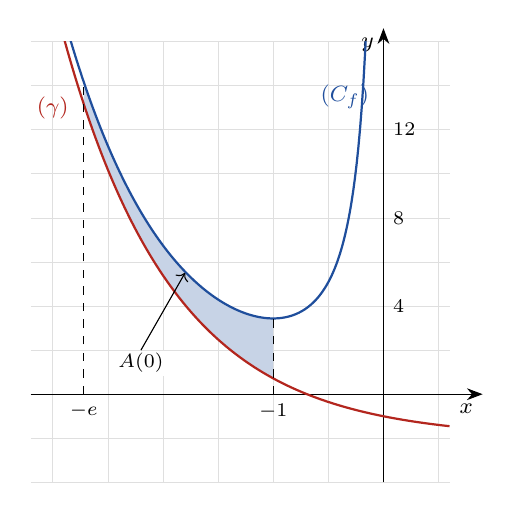
\begin{tikzpicture}[x=1.4cm,y=0.28cm,font=\footnotesize]
\draw[gray!25,very thin,xstep=0.5,ystep=2] (-3.2,-4) grid (0.6,16);
\draw[-{Stealth[length=2mm]}] (-3.2,0)--(0.9,0) node[below left]{$x$};
\draw[-{Stealth[length=2mm]}] (0,-4)--(0,16.6) node[below left]{$y$};
\begin{scope}\clip (-3.2,-4) rectangle (0.6,16);
\fill[cDef!25] plot[domain=-2.71828:-1,samples=80](\x,{exp(-\x)-2-2.71828/\x}) -- plot[domain=-1:-2.71828,samples=80](\x,{exp(-\x)-2}) -- cycle;
\draw[cDef,thick,domain=-3.2:-0.15,samples=200] plot(\x,{exp(-\x)-2-2.71828/\x});
\draw[cDef,thick,domain=0.15:0.6,samples=50] plot(\x,{exp(-\x)-2-2.71828/\x});
\draw[cThm,thick,domain=-3.2:0.6,samples=150] plot(\x,{exp(-\x)-2});
\draw[dashed] (-2.71828,0)--(-2.71828,14.2) (-1,0)--(-1,3.5);
\end{scope}
\draw[->] (-2.2,2) node[below,font=\scriptsize,fill=white,inner sep=1pt]{$A(0)$} -- (-1.8,5.5);
\node[below,font=\scriptsize] at (-2.71828,0){$-e$};
\node[below,font=\scriptsize] at (-1,0){$-1$};
\foreach \t in {4,8,12} \node[right,font=\scriptsize] at (0,\t){$\t$};
\node[cDef] at (-0.35,13.5){$(C_f)$};
\node[cThm] at (-3.0,13){$(\gamma)$};
\end{tikzpicture}\end{LTR}\end{center}
\begin{center}\small (الحيز من أجل $n=0$: بين $x=-e$ و $x=-1$)\end{center}
\end{hal}

% ===================== 2017 -- 2 =====================
\begin{tamrin}{بكالوريا 2017 -- الدورة العادية -- الموضوع الثاني -- علوم تجريبية}
$f$ الدالة العددية المعرفة على $\R$ بـ: $f(x)=2-x^2e^{1-x}$، و $(C_f)$ تمثيلها البياني.
\QQ{1} $F$ الدالة المعرفة على $\R$ بـ: $F(x)=2x+(x^2+2x+2)e^{1-x}$.
تحقق أن $F$ دالة أصلية للدالة $f$ على $\R$، ثم أحسب مساحة الحيز المستوي المحدد بالمنحنى $(C_f)$، حامل محور الفواصل والمستقيمين اللذين معادلتاهما: $x=0$ و $x=1$.
\end{tamrin}

\begin{hal}
\QQ{1} \textbf{التحقق:} $F$ قابلة للاشتقاق على $\R$، و $(e^{1-x})'=-e^{1-x}$:
\[F'(x)=2+(2x+2)e^{1-x}-(x^2+2x+2)e^{1-x}=2+(2x+2-x^2-2x-2)e^{1-x}=2-x^2e^{1-x}=f(x)\]
إذن \bxt{$F$ دالة أصلية للدالة $f$ على $\R$}.

\textbf{إشارة $f$ على $[0;1]$:} نضع $\psi(x)=x^2e^{1-x}$، $\psi'(x)=(2x-x^2)e^{1-x}=x(2-x)e^{1-x}\ge0$ على $[0;1]$، إذن $\psi$ متزايدة على $[0;1]$ ومنه $\psi(x)\le\psi(1)=1$، وبالتالي $f(x)=2-\psi(x)\ge2-1=1>0$.
\begin{TAB}
\tkzTabInit[lgt=3.2,espcl=5]{$x$ /0.8,$f(x)$ /0.8,\ar{الوضع النسبي} /1}{$0$,$1$}
\tkzTabLine{,+,}
\tkzTabLine{,\hbox{\ar{\footnotesize $(C_f)$ فوق محور الفواصل}},}
\end{TAB}
\[\mathcal{A}=\int_0^1|f(x)|\,dx=\big[F(x)\big]_0^1=F(1)-F(0)=(2+5e^0)-(0+2e)\]
\[\bx{\mathcal{A}=(7-2e)\ \text{u.a}\approx1{,}56\ \text{u.a}}\]
\begin{GR}{-1}{5}{-1}{3}{1}
\fill[cDef!25,domain=0:1,samples=60] (0,0) -- plot(\x,{2-\x*\x*exp(1-\x)}) -- (1,0) -- cycle;
\draw[cDef,thick,domain=-0.8:5,samples=150] plot(\x,{2-\x*\x*exp(1-\x)});
\draw[dashed] (1,0)--(1,1);
\node at (0.5,0.7){$\mathcal{A}$};
\node[cDef] at (4.4,1.9){$(C_f)$};
\Ticks{1,2,3,4}{1,2}
\end{GR}
\end{hal}

% ===================== 2016 -- 2 -- 1 =====================
\begin{tamrin}{بكالوريا 2016 -- الدورة الثانية -- الموضوع الأول -- علوم تجريبية}
$f$ الدالة المعرفة على المجال $]-1;+\infty[$ بـ: $f(x)=\dfrac{e}{x+1}+\dfrac{\ln(x+1)}{(x+1)^2}$، و $(C_f)$ تمثيلها البياني.
\QQ{1} بيّن أن الدالة $x\mapsto\dfrac{-1}{x+1}\big[1+\ln(x+1)\big]$ هي دالة أصلية للدالة $x\mapsto\dfrac{\ln(x+1)}{(x+1)^2}$ على المجال $]-1;+\infty[$.
\QQ{2} أحسب مساحة الحيز المستوي المحدد بحامل محور الفواصل والمنحنى $(C_f)$ والمستقيمين اللذين معادلتاهما $x=0$ و $x=1$.
\end{tamrin}

\begin{hal}
\QQ{1} نضع $G(x)=-\dfrac{1+\ln(x+1)}{x+1}$، وهي قابلة للاشتقاق على $]-1;+\infty[$:
\[G'(x)=-\frac{\frac1{x+1}(x+1)-\big(1+\ln(x+1)\big)\cdot1}{(x+1)^2}=-\frac{1-1-\ln(x+1)}{(x+1)^2}=\frac{\ln(x+1)}{(x+1)^2}\]
إذن \bxt{$G$ دالة أصلية للدالة $x\mapsto\frac{\ln(x+1)}{(x+1)^2}$ على $]-1;+\infty[$}.

\QQ{2} على $[0;1]$: $x+1>0$، و $x+1\ge1$ إذن $\ln(x+1)\ge0$؛ ومنه $f(x)>0$.
\begin{TAB}
\tkzTabInit[lgt=3.2,espcl=5]{$x$ /0.8,$f(x)$ /0.8,\ar{الوضع النسبي} /1}{$0$,$1$}
\tkzTabLine{,+,}
\tkzTabLine{,\hbox{\ar{\footnotesize $(C_f)$ فوق محور الفواصل}},}
\end{TAB}
دالة أصلية لـ $\frac{e}{x+1}$ هي $e\ln(x+1)$، إذن:
\[\mathcal{A}=\int_0^1f(x)\,dx=\big[e\ln(x+1)\big]_0^1+\big[G(x)\big]_0^1=e\ln2+\Big(-\frac{1+\ln2}{2}+1\Big)\]
\[\bx{\mathcal{A}=\Big(e\ln2+\frac{1-\ln2}{2}\Big)\ \text{u.a}\approx2{,}04\ \text{u.a}}\]
\begin{GR}{-1}{4}{-1}{3.5}{1.1}
\fill[cDef!25,domain=0:1,samples=60] (0,0) -- plot(\x,{2.71828/(\x+1)+ln(\x+1)/((\x+1)*(\x+1))}) -- (1,0) -- cycle;
\draw[cDef,thick,domain=-0.86:4,samples=200] plot(\x,{2.71828/(\x+1)+ln(\x+1)/((\x+1)*(\x+1))});
\draw[dashed,gray] (-1,-1)--(-1,3.5);
\draw[dashed] (1,0)--(1,1.53);
\node at (0.5,1){$\mathcal{A}$};
\node[cDef] at (3,1.2){$(C_f)$};
\Ticks{1,2,3}{1,2,3}
\end{GR}
\end{hal}

% ===================== 2016 -- 1 -- 1 =====================
\begin{tamrin}{بكالوريا 2016 -- الدورة الأولى -- الموضوع الأول -- علوم تجريبية}
$f$ الدالة المعرفة على المجال $]0;+\infty[$ بـ: $f(x)=\dfrac{\ln x}{x}+x-1$، و $(C_f)$ تمثيلها البياني.
\QQ{1}
\begin{sq}
\qa أوجد دالة أصلية للدالة $x\mapsto\dfrac{\ln x}{x}$ على المجال $]0;+\infty[$.
\qb أحسب بـ $I_n$ مساحة الحيز المستوي المحدد بالمنحنى $(C_f)$، المستقيم $(\Delta)$ ذي المعادلة $y=x-1$ والمستقيمين اللذين معادلتاهما $x=1$ و $x=n$ حيث $n$ عدد طبيعي ($n>1$).
\qc عيّن أصغر عدد طبيعي $n_0$ بحيث إذا كان $n>n_0$ فإن: $I_n>2$.
\end{sq}
\end{tamrin}

\begin{hal}
\QQ{1}
\pa $\dfrac{\ln x}{x}=\dfrac1x\cdot\ln x$ من الشكل $u'u$ مع $u(x)=\ln x$، ودالة أصلية لها $\dfrac{u^2}{2}$:
\bx{x\mapsto\frac{(\ln x)^2}{2}}.

\pb من أجل $x>0$: $f(x)-(x-1)=\dfrac{\ln x}{x}$، وعلى $[1;n]$: $\ln x\ge0$ و $x>0$ إذن $\dfrac{\ln x}{x}\ge0$.
\begin{TAB}
\tkzTabInit[lgt=3.2,espcl=5]{$x$ /0.8,$f(x)-(x-1)$ /0.8,\ar{الوضع النسبي} /1}{$1$,$n$}
\tkzTabLine{z,+,}
\tkzTabLine{,\hbox{\ar{\footnotesize $(C_f)$ فوق $(\Delta)$}},}
\end{TAB}
\[I_n=\int_1^n\big|f(x)-(x-1)\big|\,dx=\int_1^n\frac{\ln x}{x}\,dx=\Big[\frac{(\ln x)^2}{2}\Big]_1^n\qquad\Rightarrow\qquad\bx{I_n=\frac{(\ln n)^2}{2}\ \text{u.a}}\]
\pc $I_n>2\Leftrightarrow(\ln n)^2>4\Leftrightarrow\ln n>2$ (لأن $n>1$ إذن $\ln n>0$) $\Leftrightarrow n>e^2\approx7{,}39$.
بما أن $n$ عدد طبيعي: $I_n>2\Leftrightarrow n\ge8\Leftrightarrow n>7$.
تحقق: $I_7=\frac{(\ln7)^2}{2}\approx1{,}89<2$ و $I_8=\frac{(\ln8)^2}{2}\approx2{,}16>2$. ومنه: \bx{n_0=7}.
\begin{GR}{-0.5}{5}{-2}{4.5}{0.9}
\fill[cDef!25] plot[domain=1:4,samples=80](\x,{ln(\x)/\x+\x-1}) -- plot[domain=4:1](\x,{\x-1}) -- cycle;
\draw[cDef,thick,domain=0.3:5,samples=150] plot(\x,{ln(\x)/\x+\x-1});
\draw[cThm,thick,domain=-0.5:5] plot(\x,{\x-1});
\draw[dashed] (4,0)--(4,3.35);
\draw[->] (3.4,0.6) node[below,font=\scriptsize]{$I_4$} -- (2.6,1.85);
\node[cDef] at (4.3,4.2){$(C_f)$};
\node[cThm] at (4.6,3.0){$(\Delta)$};
\Ticks{1,2,3,4}{-1,1,2,3,4}
\end{GR}
\begin{center}\small (الشكل من أجل $n=4$)\end{center}
\end{hal}

% ===================== 2016 -- 1 -- 2 =====================
\begin{tamrin}{بكالوريا 2016 -- الدورة الأولى -- الموضوع الثاني -- علوم تجريبية}
$f$ الدالة المعرفة على $\R$ بـ: $f(x)=-x+(x^2+3x+2)e^{-x}$، و $(C_f)$ تمثيلها البياني.
$h$ و $H$ الدالتان المعرفتان على $\R$ كما يلي: $h(x)=x+f(x)$ و $H(x)=(ax^2+bx+c)e^{-x}$.
\QQ{1} عيّن الأعداد الحقيقية $a$، $b$ و $c$ بحيث تكون الدالة $H$ دالة أصلية للدالة $h$ على $\R$.
\QQ{2}
\begin{sq}
\qa أحسب التكامل التالي: $A(\lambda)=\displaystyle\int_0^\lambda h(x)\,dx$، حيث $\lambda$ عدد حقيقي موجب تماما، وفسّر النتيجة هندسيا.
\qb أحسب $\lim\limits_{\lambda\to+\infty}A(\lambda)$.
\end{sq}
\end{tamrin}

\begin{hal}
\QQ{1} $h(x)=x+f(x)=(x^2+3x+2)e^{-x}$. $H$ قابلة للاشتقاق على $\R$:
\[H'(x)=(2ax+b)e^{-x}-(ax^2+bx+c)e^{-x}=\big(-ax^2+(2a-b)x+(b-c)\big)e^{-x}\]
$H$ دالة أصلية لـ $h$ يعني $H'(x)=h(x)$ من أجل كل $x$، وبالمطابقة:
\[\begin{cases}-a=1\\2a-b=3\\b-c=2\end{cases}\ \Longrightarrow\ \bx{a=-1\ ;\ b=-5\ ;\ c=-7}\]
إذن $H(x)=(-x^2-5x-7)e^{-x}$.

\QQ{2}
\pa
\[A(\lambda)=\big[H(x)\big]_0^\lambda=(-\lambda^2-5\lambda-7)e^{-\lambda}-(-7)\qquad\Rightarrow\qquad\bx{A(\lambda)=7-(\lambda^2+5\lambda+7)e^{-\lambda}}\]
\textbf{التفسير الهندسي:} $h(x)=f(x)-(-x)$، ومن أجل $x\ge0$: $x^2+3x+2=(x+1)(x+2)>0$ و $e^{-x}>0$، إذن $h(x)>0$.
\begin{TAB}
\tkzTabInit[lgt=3.2,espcl=5]{$x$ /0.8,$f(x)-(-x)$ /0.8,\ar{الوضع النسبي} /1}{$0$,$\lambda$}
\tkzTabLine{,+,}
\tkzTabLine{,\hbox{\ar{\footnotesize $(C_f)$ فوق المستقيم $y=-x$}},}
\end{TAB}
إذن $A(\lambda)=\displaystyle\int_0^\lambda|f(x)-(-x)|\,dx$، ومنه:

\bxt{$A(\lambda)$ مساحة الحيز المحدد بـ $(C_f)$ والمستقيمات $y=-x$، $x=0$، $x=\lambda$ (بـ u.a)}

\pb $\lim\limits_{\lambda\to+\infty}\lambda^2e^{-\lambda}=0$، $\lim\limits_{\lambda\to+\infty}\lambda e^{-\lambda}=0$ و $\lim\limits_{\lambda\to+\infty}e^{-\lambda}=0$ (التزايد المقارن)، ومنه:
\[\bx{\lim_{\lambda\to+\infty}A(\lambda)=7\ \text{u.a}}\]
\begin{GR}{-2.5}{6}{-6}{4}{0.65}
\fill[cDef!25] plot[domain=0:4,samples=80](\x,{-\x+(\x*\x+3*\x+2)*exp(-\x)}) -- plot[domain=4:0](\x,{-\x}) -- cycle;
\draw[cDef,thick,domain=-2.4:6,samples=200] plot(\x,{-\x+(\x*\x+3*\x+2)*exp(-\x)});
\draw[cThm,thick,domain=-2.5:6] plot(\x,{-\x});
\draw[dashed] (4,-4)--(4,0);
\node at (1.2,0.1){$A(\lambda)$};
\node[below,font=\scriptsize] at (4.25,0){$\lambda$};
\node[cDef] at (-1.6,3.3){$(C_f)$};
\node[cThm] at (5.3,-4.4){$y=-x$};
\Ticks{-2,-1,1,2,3,5}{-5,-4,-3,-2,-1,1,2,3}
\end{GR}
\begin{center}\small (الشكل من أجل $\lambda=4$)\end{center}
\end{hal}

% ===================== 2015 -- 1 =====================
\begin{tamrin}{بكالوريا 2015 -- الموضوع الأول -- علوم تجريبية}
$f$ الدالة المعرفة على $]0;+\infty[$ بـ: $f(x)=\Big(1-\dfrac1x\Big)(\ln x-2)$.
$F$ الدالة الأصلية للدالة $f$ على المجال $]0;+\infty[$ والتي تحقق: $F(1)=-3$.
\QQ{1} بيّن أن منحنى الدالة $F$ يقبل مماسين موازيين لحامل محور الفواصل في نقطتين يطلب تعيين فاصلتيهما.
\QQ{2} بيّن أن $x\mapsto x\ln x-x$ هي دالة أصلية للدالة $x\mapsto\ln x$ على $]0;+\infty[$، ثم استنتج عبارة الدالة $F$.
\end{tamrin}

\begin{hal}
\QQ{1} $F$ دالة أصلية لـ $f$ إذن $F'(x)=f(x)$. المماس لمنحنى $F$ يوازي محور الفواصل عند النقطة ذات الفاصلة $x_0$ إذا وفقط إذا كان $F'(x_0)=0$، أي $f(x_0)=0$:
$\Big(1-\dfrac1x\Big)(\ln x-2)=0$ يعني $1-\dfrac1x=0$ أو $\ln x-2=0$، أي $x=1$ أو $x=e^2$ (كلاهما من $]0;+\infty[$).


\bxt{المنحنى يقبل مماسين أفقيين عند النقطتين ذواتي الفاصلتين $1$ و $e^2$}

\QQ{2} $(x\ln x-x)'=\ln x+x\cdot\frac1x-1=\ln x$، إذن \bxt{$x\mapsto x\ln x-x$ دالة أصلية لـ $\ln$ على $]0;+\infty[$}.

\textbf{استنتاج $F$:} ننشر: $f(x)=\ln x-2-\dfrac{\ln x}{x}+\dfrac2x$.
\begin{itemize}
\item دالة أصلية لـ $\ln x$ هي $x\ln x-x$، ولـ $-2$ هي $-2x$.
\item $\dfrac{\ln x}{x}$ من الشكل $u'u$ ($u=\ln x$)، دالة أصلية لها $\frac{(\ln x)^2}{2}$؛ ولـ $\frac2x$ هي $2\ln x$.
\end{itemize}
إذن $F(x)=x\ln x-3x-\dfrac{(\ln x)^2}{2}+2\ln x+k$ حيث $k\in\R$. و $F(1)=0-3-0+0+k=-3$ يعطي $k=0$:
\[\bx{F(x)=x\ln x-3x-\frac{(\ln x)^2}{2}+2\ln x}\]
\end{hal}

% ===================== 2015 -- 2 =====================
\begin{tamrin}{بكالوريا 2015 -- الموضوع الثاني -- علوم تجريبية}
$f$ الدالة العددية المعرفة على $\R$ بـ: $f(x)=xe^{2x+2}-x+1$.
\QQ{1} تحقق أنه من أجل كل $x$ من $\R$: $2f(x)+f'(x)-f''(x)=1-2x-3e^{2x+2}$.
\QQ{2} استنتج دالة أصلية للدالة $f$ على $\R$.
\end{tamrin}

\begin{hal}
\QQ{1} من أجل كل $x\in\R$:
\[f'(x)=e^{2x+2}+2xe^{2x+2}-1=(2x+1)e^{2x+2}-1\]
\[f''(x)=2e^{2x+2}+2(2x+1)e^{2x+2}=(4x+4)e^{2x+2}\]
\[2f(x)+f'(x)-f''(x)=\big(2x+2x+1-4x-4\big)e^{2x+2}+(-2x+2)-1\]
\[\bx{2f(x)+f'(x)-f''(x)=1-2x-3e^{2x+2}}\]
\QQ{2} من العلاقة السابقة: $f(x)=\dfrac12\Big[1-2x-3e^{2x+2}-f'(x)+f''(x)\Big]$.
دالة أصلية لـ $f'$ هي $f$، ولـ $f''$ هي $f'$، ولـ $e^{2x+2}$ هي $\frac12e^{2x+2}$؛ إذن دالة أصلية لـ $f$:
\[F(x)=\frac12\Big[x-x^2-\frac32e^{2x+2}-f(x)+f'(x)\Big]\]
مع $-f(x)+f'(x)=-xe^{2x+2}+x-1+(2x+1)e^{2x+2}-1=(x+1)e^{2x+2}+x-2$:
\[F(x)=\frac12\Big[-x^2+2x-2+\Big(x-\frac12\Big)e^{2x+2}\Big]\]
\[\bx{F(x)=\frac{2x-1}{4}e^{2x+2}-\frac{x^2}{2}+x-1}\]
تحقق: $F'(x)=\frac12e^{2x+2}+\frac{2x-1}{2}e^{2x+2}-x+1=xe^{2x+2}-x+1=f(x)$ \ok.
\end{hal}

% ===================== 2012 -- 1 =====================
\begin{tamrin}{بكالوريا 2012 -- الموضوع الأول -- علوم تجريبية}
$f$ الدالة المعرفة على المجال $]-\infty;0[$ كما يلي: $f(x)=x+5+6\ln\Big(\dfrac{x}{x-1}\Big)$، و $(C_f)$ تمثيلها البياني.
لتكن $g$ الدالة المعرفة على $]-\infty;0[$ كما يلي: $g(x)=\dfrac{x^2}{2}+5x+6x\ln\Big(\dfrac{x}{x-1}\Big)+6\ln(1-x)$.
بيّن أن $g$ دالة أصلية للدالة $f$ على المجال $]-\infty;0[$.
\end{tamrin}
\begin{molahada}
في نص المصدر: $g(x)=\dfrac{x^2}{2}+5x+6x\ln\Big(\dfrac{x}{x-1}\Big)$، وهذه الدالة ليست دالة أصلية لـ $f$ لأن مشتقتها $f(x)-\dfrac{6}{x-1}$. صحّحنا العبارة بإضافة الحد $6\ln(1-x)$.
\end{molahada}

\begin{hal}
من أجل $x<0$: $x<0$ و $x-1<0$ إذن $\dfrac{x}{x-1}>0$، و $1-x>0$؛ فـ $g$ معرفة وقابلة للاشتقاق على $]-\infty;0[$.
\[\Big(\frac{x}{x-1}\Big)'=\frac{(x-1)-x}{(x-1)^2}=\frac{-1}{(x-1)^2}\ \Rightarrow\ \Big[\ln\frac{x}{x-1}\Big]'=\frac{-1}{(x-1)^2}\cdot\frac{x-1}{x}=\frac{-1}{x(x-1)}\]
\[\Big[6x\ln\frac{x}{x-1}\Big]'=6\ln\frac{x}{x-1}+6x\cdot\frac{-1}{x(x-1)}=6\ln\frac{x}{x-1}-\frac{6}{x-1}\]
\[\big[6\ln(1-x)\big]'=6\cdot\frac{-1}{1-x}=\frac{6}{x-1}\]
إذن:
\[g'(x)=x+5+6\ln\frac{x}{x-1}-\frac6{x-1}+\frac6{x-1}=x+5+6\ln\frac{x}{x-1}=f(x)\]
\bxt{$g$ دالة أصلية للدالة $f$ على $]-\infty;0[$}
\end{hal}

% ===================== 2012 -- 2 =====================
\begin{tamrin}{بكالوريا 2012 -- الموضوع الثاني -- علوم تجريبية}
$g$ الدالة العددية المعرفة على $\R$ بـ: $g(x)=1-xe^x$.
\QQ{1} $h$ الدالة المعرفة على $\R$ كما يلي: $h(x)=(ax+b)e^x$.
\begin{sq}
\qa عيّن العددين الحقيقيين $a$ و $b$ بحيث تكون $h$ دالة أصلية للدالة $x\mapsto xe^x$ على $\R$.
\qb استنتج دالة أصلية للدالة $g$ على $\R$.
\end{sq}
\end{tamrin}

\begin{hal}
\QQ{1}
\pa $h'(x)=ae^x+(ax+b)e^x=(ax+a+b)e^x$. $h$ دالة أصلية لـ $x\mapsto xe^x$ يعني $(ax+a+b)e^x=xe^x$ لكل $x$، وبالمطابقة: $a=1$ و $a+b=0$:
\[\bx{a=1\ ;\ b=-1}\qquad h(x)=(x-1)e^x\]
\pb $g(x)=1-xe^x$، ودالة أصلية لـ $1$ هي $x$، ولـ $xe^x$ هي $h$؛ إذن:
\[\bx{G(x)=x-(x-1)e^x}\]
(وكل الدوال الأصلية: $x-(x-1)e^x+k$، $k\in\R$.) تحقق: $G'(x)=1-e^x-(x-1)e^x=1-xe^x=g(x)$ \ok.
\end{hal}

% ===================== 2011 -- 1 =====================
\begin{tamrin}{بكالوريا 2011 -- الموضوع الأول -- علوم تجريبية}
$g$ الدالة المعرفة على $\R-\{-1\}$ بـ: $g(x)=\dfrac{x-1}{x+1}$، و $f$ الدالة المعرفة على المجال $]1;+\infty[$ بـ: $f(x)=\dfrac{x-1}{x+1}+\ln\Big(\dfrac{x-1}{x+1}\Big)$.
\QQ{1} $\alpha$ عدد حقيقي. بيّن أن الدالة $x\mapsto(x-\alpha)\ln(x-\alpha)-x$ هي دالة أصلية للدالة $x\mapsto\ln(x-\alpha)$ على المجال $]\alpha;+\infty[$.
\QQ{2} تحقق أنه من أجل كل عدد حقيقي $x$ من المجال $]1;+\infty[$: $g(x)=1-\dfrac{2}{x+1}$، ثم عيّن دالة أصلية للدالة $f$ على المجال $]1;+\infty[$.
\end{tamrin}

\begin{hal}
\QQ{1} من أجل $x>\alpha$:
\[\big[(x-\alpha)\ln(x-\alpha)-x\big]'=1\cdot\ln(x-\alpha)+(x-\alpha)\cdot\frac1{x-\alpha}-1=\ln(x-\alpha)\]
\bxt{$x\mapsto(x-\alpha)\ln(x-\alpha)-x$ دالة أصلية لـ $x\mapsto\ln(x-\alpha)$ على $]\alpha;+\infty[$}

\QQ{2} $1-\dfrac2{x+1}=\dfrac{x+1-2}{x+1}=\dfrac{x-1}{x+1}=g(x)$ \ok.

من أجل $x>1$: $x-1>0$ و $x+1>0$، إذن $\ln\dfrac{x-1}{x+1}=\ln(x-1)-\ln(x+1)$، ومنه:
\[f(x)=1-\frac2{x+1}+\ln(x-1)-\ln(x+1)\]
\begin{itemize}
\item دالة أصلية لـ $1-\frac2{x+1}$ هي $x-2\ln(x+1)$.
\item حسب 1 مع $\alpha=1$: دالة أصلية لـ $\ln(x-1)$ هي $(x-1)\ln(x-1)-x$.
\item حسب 1 مع $\alpha=-1$: دالة أصلية لـ $\ln(x+1)$ هي $(x+1)\ln(x+1)-x$.
\end{itemize}
\[F(x)=x-2\ln(x+1)+(x-1)\ln(x-1)-x-(x+1)\ln(x+1)+x\]
\[\bx{F(x)=x+(x-1)\ln(x-1)-(x+3)\ln(x+1)}\]
\end{hal}

% ===================== 2011 -- 2 =====================
\begin{tamrin}{بكالوريا 2011 -- الموضوع الثاني -- علوم تجريبية}
$f$ الدالة المعرفة على $\R$ بـ: $f(x)=e^x-ex-1$، و $(C_f)$ تمثيلها البياني. نقبل أن المعادلة $f(x)=0$ تقبل حلين $0$ و $\alpha$ حيث $\alpha\in]1{,}75;1{,}76[$.
\QQ{1} أحسب بدلالة $\alpha$ المساحة $A(\alpha)$ للحيز المستوي المحدد بالمنحنى $(C_f)$، حامل محور الفواصل والمستقيمين اللذين معادلتاهما: $x=0$، $x=\alpha$.
\QQ{2} أثبت أن: $A(\alpha)=\Big(\dfrac12e\alpha^2-e\alpha+\alpha\Big)\,ua$ (\,$ua$ هي وحدة المساحات).
\end{tamrin}

\begin{hal}
\QQ{1} \textbf{إشارة $f$ على $[0;\alpha]$:} $f'(x)=e^x-e$، تنعدم عند $x=1$؛ $f'(x)<0$ على $]-\infty;1[$ و $f'(x)>0$ على $]1;+\infty[$.
\begin{itemize}
\item على $[0;1]$: $f$ متناقصة، إذن $f(x)\le f(0)=0$.
\item على $[1;\alpha]$: $f$ متزايدة، إذن $f(x)\le f(\alpha)=0$.
\end{itemize}
\begin{TAB}
\tkzTabInit[lgt=3.2,espcl=5]{$x$ /0.8,$f(x)$ /0.8,\ar{الوضع النسبي} /1}{$0$,$\alpha$}
\tkzTabLine{z,-,z}
\tkzTabLine{,\hbox{\ar{\footnotesize $(C_f)$ تحت محور الفواصل}},}
\end{TAB}
إذن $|f(x)|=-f(x)$ على $[0;\alpha]$:
\[A(\alpha)=-\int_0^\alpha\big(e^x-ex-1\big)\,dx=-\Big[e^x-\frac e2x^2-x\Big]_0^\alpha=-\Big(e^\alpha-\frac e2\alpha^2-\alpha-1\Big)\]
\[\bx{A(\alpha)=-e^\alpha+\frac e2\alpha^2+\alpha+1\ \text{u.a}}\]
\QQ{2} $f(\alpha)=0$ يعني $e^\alpha=e\alpha+1$، نعوض:
\[A(\alpha)=-(e\alpha+1)+\frac e2\alpha^2+\alpha+1\qquad\Rightarrow\qquad\bx{A(\alpha)=\Big(\frac12e\alpha^2-e\alpha+\alpha\Big)\,ua\approx1{,}16\,ua}\]
\begin{GR}{-2}{2.3}{-1.5}{3}{1.3}
\fill[cDef!25,domain=0:1.7508,samples=80] (0,0) -- plot(\x,{exp(\x)-2.71828*\x-1}) -- (1.7508,0) -- cycle;
\draw[cDef,thick,domain=-2:2.3,samples=150] plot(\x,{exp(\x)-2.71828*\x-1});
\node at (0.9,-0.45){$A(\alpha)$};
\node[above,font=\scriptsize] at (1.85,0){$\alpha$};
\node[cDef] at (-1.4,2.8){$(C_f)$};
\Ticks{-1,1}{-1,1,2}
\end{GR}
\end{hal}

% ===================== 2009 -- 1 =====================
\begin{tamrin}{بكالوريا 2009 -- الموضوع الأول -- علوم تجريبية}
$k$ الدالة المعرفة على $\R-\{-1\}$ كما يلي: $k(x)=|x|+\dfrac4{x+1}$، و $(C_k)$ تمثيلها البياني.
\QQ{1} أحسب مساحة الحيز المستوي المحدد بالمنحنى $(C_k)$ والمستقيمات التي معادلاتها: $y=0$، $x=\dfrac12$، $x=-\dfrac12$.
\end{tamrin}

\begin{hal}
\QQ{1} على $\big[-\frac12;\frac12\big]$: $|x|\ge0$ و $x+1\ge\frac12>0$ إذن $k(x)>0$.
\begin{TAB}
\tkzTabInit[lgt=3.2,espcl=5]{$x$ /0.8,$k(x)$ /0.8,\ar{الوضع النسبي} /1}{$-\frac12$,$\frac12$}
\tkzTabLine{,+,}
\tkzTabLine{,\hbox{\ar{\footnotesize $(C_k)$ فوق محور الفواصل}},}
\end{TAB}
بسبب القيمة المطلقة نستعمل علاقة شال: $|x|=-x$ على $\big[-\frac12;0\big]$ و $|x|=x$ على $\big[0;\frac12\big]$:
\[\mathcal{A}=\int_{-\frac12}^{0}\Big(-x+\frac4{x+1}\Big)dx+\int_0^{\frac12}\Big(x+\frac4{x+1}\Big)dx\]
\[=\Big[-\frac{x^2}{2}+4\ln(x+1)\Big]_{-\frac12}^{0}+\Big[\frac{x^2}{2}+4\ln(x+1)\Big]_0^{\frac12}=\Big(\frac18-4\ln\frac12\Big)+\Big(\frac18+4\ln\frac32\Big)\]
\[=\frac14+4\ln2+4\ln3-4\ln2\qquad\Rightarrow\qquad\bx{\mathcal{A}=\Big(\frac14+4\ln3\Big)\ \text{u.a}\approx4{,}64\ \text{u.a}}\]
\begin{GR}{-1.5}{3}{-1}{9}{0.6}
\fill[cDef!25] (-0.5,0) -- plot[domain=-0.5:0.5,samples=100](\x,{abs(\x)+4/(\x+1)}) -- (0.5,0) -- cycle;
\draw[cDef,thick,domain=-0.6:3,samples=200] plot(\x,{abs(\x)+4/(\x+1)});
\draw[dashed,gray] (-1,-1)--(-1,9);
\draw[dashed] (-0.5,0)--(-0.5,8.5);
\node at (0.05,1.8){$\mathcal{A}$};
\node[cDef] at (2.3,5){$(C_k)$};
\Ticks{1,2}{2,4,6,8}
\node[below,font=\scriptsize] at (-1,0){$-1$};
\end{GR}
\end{hal}

% ===================== 2009 -- 2 =====================
\begin{tamrin}{بكالوريا 2009 -- الموضوع الثاني -- علوم تجريبية}
$f$ الدالة العددية المعرفة على $]-1;+\infty[$ كما يلي: $f(x)=x-1-\dfrac{\ln(x+1)}{x+1}$، و $(C_f)$ تمثيلها البياني.
\QQ{1} أحسب مساحة الحيز المستوي المحدود بالمنحنى $(C_f)$ والمستقيمات التي معادلاتها: $y=x-1$، $x=0$ و $x=1$.
\end{tamrin}

\begin{hal}
\QQ{1} $f(x)-(x-1)=-\dfrac{\ln(x+1)}{x+1}$. على $[0;1]$: $x+1\ge1$ إذن $\ln(x+1)\ge0$، و $x+1>0$؛ ومنه $f(x)-(x-1)\le0$.
\begin{TAB}
\tkzTabInit[lgt=3.2,espcl=5]{$x$ /0.8,$f(x)-(x-1)$ /0.8,\ar{الوضع النسبي} /1}{$0$,$1$}
\tkzTabLine{z,-,}
\tkzTabLine{,\hbox{\ar{\footnotesize $(C_f)$ تحت المستقيم $y=x-1$}},}
\end{TAB}
$\dfrac{\ln(x+1)}{x+1}$ من الشكل $u'u$ مع $u(x)=\ln(x+1)$:
\[\mathcal{A}=\int_0^1\big|f(x)-(x-1)\big|\,dx=\int_0^1\frac{\ln(x+1)}{x+1}\,dx=\Big[\frac{(\ln(x+1))^2}{2}\Big]_0^1\]
\[\bx{\mathcal{A}=\frac{(\ln2)^2}{2}\ \text{u.a}\approx0{,}24\ \text{u.a}}\]
\begin{GR}{-1}{3}{-2.5}{2.5}{1.1}
\fill[cDef!25] plot[domain=0:1,samples=60](\x,{\x-1}) -- plot[domain=1:0,samples=60](\x,{\x-1-ln(\x+1)/(\x+1)}) -- cycle;
\draw[cDef,thick,domain=-0.86:3,samples=200] plot(\x,{\x-1-ln(\x+1)/(\x+1)});
\draw[cThm,thick,domain=-1:3] plot(\x,{\x-1});
\draw[dashed,gray] (-1,-2.5)--(-1,2.5);
\draw[dashed] (1,0)--(1,-0.35);
\draw[->] (1.2,-1.5) node[below,font=\scriptsize]{$\mathcal{A}$} -- (0.55,-0.6);
\node[cDef] at (2.6,1.0){$(C_f)$};
\node[cThm] at (2.2,1.8){$y=x-1$};
\Ticks{1,2}{-2,-1,1,2}
\end{GR}
\end{hal}

% ===================== 2008 -- 1 =====================
\begin{tamrin}{بكالوريا 2008 -- الموضوع الأول -- علوم تجريبية}
$g$ الدالة العددية المعرفة على المجال $[-2;+\infty[$ كما يلي: $g(x)=(-x-1)e^{-x}+1$.
\QQ{1} $H$ الدالة العددية المعرفة على المجال $[-2;+\infty[$ كما يلي: $H(x)=(\alpha x+\beta)e^{-x}$ حيث $\alpha$ و $\beta$ عددان حقيقيان.
\begin{sq}
\qa عيّن $\alpha$ و $\beta$ بحيث تكون $H$ دالة أصلية للدالة: $x\mapsto g(x)-1$.
\qb استنتج الدالة الأصلية للدالة $g$ والتي تنعدم عند القيمة $0$.
\end{sq}
\end{tamrin}

\begin{hal}
\QQ{1}
\pa $g(x)-1=(-x-1)e^{-x}$، و $H'(x)=\alpha e^{-x}-(\alpha x+\beta)e^{-x}=(-\alpha x+\alpha-\beta)e^{-x}$.
بالمطابقة: $-\alpha=-1$ و $\alpha-\beta=-1$، إذن:
\[\bx{\alpha=1\ ;\ \beta=2}\qquad H(x)=(x+2)e^{-x}\]
\pb $g(x)=\big(g(x)-1\big)+1$، فالدوال الأصلية لـ $g$ هي $G(x)=(x+2)e^{-x}+x+k$، $k\in\R$.
$G(0)=0$ يعني $2+k=0$ أي $k=-2$:
\[\bx{G(x)=(x+2)e^{-x}+x-2}\]
\end{hal}

% ===================== 2008 -- 2 =====================
\begin{tamrin}{بكالوريا 2008 -- الموضوع الثاني -- علوم تجريبية}
$f$ الدالة العددية المعرفة على المجال $]-1;+\infty[$ بـ: $f(x)=\dfrac{x^3+3x^2+3x+2}{(x+1)^2}$.
\QQ{1} أكتب $f(x)$ على الشكل $f(x)=x+a+\dfrac{b}{(x+1)^2}$ حيث $a$ و $b$ عددان حقيقيان.
\QQ{2} عيّن $F$ الدالة الأصلية للدالة $f$ على المجال $]-1;+\infty[$ والتي تحقق $F(1)=2$.
\end{tamrin}
\begin{molahada}
في نص المصدر كُتب المقام $(x-1)^2$ في السؤال 1، والصواب $(x+1)^2$ (مقام $f$، والدالة معرفة عند $x=1$).
\end{molahada}

\begin{hal}
\QQ{1} نوحد المقامات:
\[x+a+\frac{b}{(x+1)^2}=\frac{(x+a)(x^2+2x+1)+b}{(x+1)^2}=\frac{x^3+(a+2)x^2+(2a+1)x+a+b}{(x+1)^2}\]
بالمطابقة مع $x^3+3x^2+3x+2$: $a+2=3$، $2a+1=3$، $a+b=2$، إذن $a=1$ و $b=1$:
\[\bx{f(x)=x+1+\frac1{(x+1)^2}}\]
(أو: $x^3+3x^2+3x+2=(x+1)^3+1$.)

\QQ{2} دالة أصلية لـ $\dfrac1{(x+1)^2}$ من الشكل $\dfrac{u'}{u^2}$ ($u=x+1$) هي $-\dfrac1{x+1}$، إذن:
$F(x)=\dfrac{x^2}{2}+x-\dfrac1{x+1}+k$. و $F(1)=\frac12+1-\frac12+k=1+k=2$ يعطي $k=1$:
\[\bx{F(x)=\frac{x^2}{2}+x-\frac1{x+1}+1}\]
\end{hal}

\section{تمارين البكالوريا -- شعبة تقني رياضي}
% ===================== التمرين: 2026 م1 =====================
\begin{tamrin}{بكالوريا 2026 -- الموضوع الأول -- تقني رياضي}
$f$ الدالة المعرفة على $\R$ بـ: $f(x)=1+\left(1-x-x^{2}\right)e^{-x}$، و $(C_f)$ تمثيلها البياني في المستوي المنسوب إلى المعلم المتعامد والمتجانس $(O;\vec{i},\vec{j})$.

\QQ{1}
\begin{sq}
\qa تحقق أن الدالة $H:x\mapsto \left(x^{2}+3x+2\right)e^{-x}$ أصلية للدالة $h:x\mapsto\left(1-x-x^{2}\right)e^{-x}$ على $\R$.
\qb $A(\alpha)$ مساحة الحيز المستوي المحدد بـ $(C_f)$ والمستقيمات التي معادلاتها: $y=0$، $x=\alpha$ و $x=0$.

احسب $A(\alpha)$ ثم بين أن: $A(\alpha)=\dfrac{4+\alpha^{3}}{1-\alpha-\alpha^{2}}$، مقدرة بوحدة المساحة.
\end{sq}
($\alpha$ عدد حقيقي يحقق $f(\alpha)=0$ و $-1{,}7<\alpha<-1{,}6$.)
\end{tamrin}

\begin{hal}
\QQ{1}
\pa الدالة $H$ قابلة للاشتقاق على $\R$ (جداء دالة كثير حدود والدالة $x\mapsto e^{-x}$). نستعمل $(uv)'=u'v+uv'$ مع $u(x)=x^2+3x+2$ و $v(x)=e^{-x}$، حيث $u'(x)=2x+3$ و $v'(x)=-e^{-x}$:
\begin{align*}
H'(x)&=(2x+3)e^{-x}+\left(x^{2}+3x+2\right)\left(-e^{-x}\right)\\
&=\left(2x+3-x^{2}-3x-2\right)e^{-x}=\left(1-x-x^{2}\right)e^{-x}=h(x).
\end{align*}
إذن \bxt{$H$ أصلية للدالة $h$ على $\R$}.

\pb \textbf{إشارة $f(x)$ على $[\alpha;0]$:} لدينا $f(x)=1+h(x)$، ومنه $f'(x)=h'(x)$، مع:
\[f'(x)=(-1-2x)e^{-x}-\left(1-x-x^{2}\right)e^{-x}=\left(x^{2}-x-2\right)e^{-x}=(x+1)(x-2)e^{-x}.\]
على $[\alpha;-1]$: $f'(x)\ge 0$، وعلى $[-1;0]$: $f'(x)\le 0$. ومنه $f$ متزايدة على $[\alpha;-1]$ من $f(\alpha)=0$ إلى $f(-1)=1+e$، ثم متناقصة على $[-1;0]$ من $1+e$ إلى $f(0)=2>0$. إذن $f(x)\ge 0$ من أجل كل $x\in[\alpha;0]$:
\begin{TAB}
\tkzTabInit[lgt=3,espcl=3.2]{$x$/1,$f(x)$/1,\ar{الوضع النسبي}/1.2}{$\alpha$,$-1$,$0$}
\tkzTabLine{z,+,t,+,}
\tkzTabLine{,\mbox{\ar{$(C_f)$ فوق $(x'x)$}},t,\mbox{\ar{$(C_f)$ فوق $(x'x)$}},}
\end{TAB}
بما أن $(C_f)$ يقع فوق محور الفواصل على $[\alpha;0]$ و $\alpha<0$:
\[A(\alpha)=\int_{\alpha}^{0}\left|f(x)\right|dx=\int_{\alpha}^{0}f(x)\,dx \ \text{u.a}\]

\begin{GR}{-2.5}{4}{-1}{4.5}{0.95}
 \Ticks{-2,-1,1,2,3}{-1,1,2,3,4}
 \fill[cDef!25,domain=-1.6972:0,samples=100] (-1.6972,0) -- plot(\x,{1+(1-\x-(\x)^2)*exp(-\x)}) -- (0,0) -- cycle;
 \draw[gray,dashed] (-2.5,1)--(4,1) node[pos=0.92,above]{$y=1$};
 \draw[cDef,very thick,domain=-2:4,samples=200,smooth] plot (\x,{1+(1-\x-(\x)^2)*exp(-\x)});
 \fill[cThm] (-1.6972,0) circle (1.6pt) node[below left]{$\alpha$};
 \node at (-0.8,1.4){$\mathcal{A}(\alpha)$};
 \node[cDef] at (2.5,0.35){$(C_f)$};
\end{GR}

\textbf{حساب التكامل:} أصلية الدالة $f=1+h$ على $\R$ هي $x\mapsto x+H(x)$، إذن:
\begin{align*}
A(\alpha)&=\Big[x+\left(x^{2}+3x+2\right)e^{-x}\Big]_{\alpha}^{0}=\left(0+2\right)-\left(\alpha+\left(\alpha^{2}+3\alpha+2\right)e^{-\alpha}\right)\\
&=2-\alpha-\left(\alpha^{2}+3\alpha+2\right)e^{-\alpha}.
\end{align*}
\textbf{استعمال $f(\alpha)=0$:} $1+\left(1-\alpha-\alpha^{2}\right)e^{-\alpha}=0$ أي $e^{-\alpha}=\dfrac{-1}{1-\alpha-\alpha^{2}}$ (لاحظ أن $1-\alpha-\alpha^2\neq 0$ لأن $f(\alpha)=0$). نعوض:
\begin{align*}
A(\alpha)&=2-\alpha+\frac{\alpha^{2}+3\alpha+2}{1-\alpha-\alpha^{2}}
=\frac{(2-\alpha)\left(1-\alpha-\alpha^{2}\right)+\alpha^{2}+3\alpha+2}{1-\alpha-\alpha^{2}}\\
&=\frac{\left(2-3\alpha-\alpha^{2}+\alpha^{3}\right)+\alpha^{2}+3\alpha+2}{1-\alpha-\alpha^{2}}.
\end{align*}
\[\bx{A(\alpha)=\frac{4+\alpha^{3}}{1-\alpha-\alpha^{2}}\ \text{u.a}}\]
\textbf{قيمة تقريبية:} $\alpha\approx -1{,}697$ يعطي $A(\alpha)\approx 4{,}85\ \text{u.a}$.
\end{hal}

% ===================== التمرين: 2026 م2 =====================
\begin{tamrin}{بكالوريا 2026 -- الموضوع الثاني -- تقني رياضي}
$f$ الدالة المعرفة على $]0;e[\,\cup\,]e;+\infty[$ بـ: $f(x)=x+\dfrac{1}{x-x\ln x}$، و $(C_f)$ تمثيلها البياني في المستوي المنسوب إلى المعلم المتعامد والمتجانس $(O;\vec{i},\vec{j})$.

\QQ{1} ادرس وضعية المنحنى $(C_f)$ بالنسبة إلى المستقيم $(\Delta)$ ذي المعادلة $y=x$.

\QQ{2} $h$ الدالة المعرفة على $]0;e[$ بـ: $h(x)=\ln(1-\ln x)$.

احسب $h'(x)$ ثم استنتج حساب $A$ مساحة الحيز المستوي المحدد بـ $(C_f)$ والمستقيمات التي معادلاتها: $y=x$، $x=\dfrac{1}{e}$ و $x=1$.
\end{tamrin}

\begin{hal}
\QQ{1} من أجل كل $x$ من $]0;e[\,\cup\,]e;+\infty[$:
\[f(x)-x=\frac{1}{x-x\ln x}=\frac{1}{x(1-\ln x)}.\]
بما أن $x>0$، فإشارة $f(x)-x$ هي إشارة $1-\ln x$: $1-\ln x>0 \iff \ln x<1\iff x<e$.
\begin{TAB}
\tkzTabInit[lgt=3,espcl=3.6]{$x$/1,$1-\ln x$/1,$f(x)-x$/1,\ar{الوضع النسبي}/1.2}{$0$,$e$,$+\infty$}
\tkzTabLine{d,+,z,-,}
\tkzTabLine{d,+,d,-,}
\tkzTabLine{d,\mbox{\ar{$(C_f)$ فوق $(\Delta)$}},d,\mbox{\ar{$(C_f)$ تحت $(\Delta)$}},}
\end{TAB}
\begin{itemize}
\item على $]0;e[$: \bxt{$(C_f)$ يقع فوق $(\Delta)$}.
\item على $]e;+\infty[$: \bxt{$(C_f)$ يقع تحت $(\Delta)$}.
\end{itemize}

\QQ{2} \textbf{حساب $h'(x)$:} من أجل $x\in]0;e[$ لدينا $1-\ln x>0$، و $h=\ln u$ مع $u(x)=1-\ln x$ و $u'(x)=-\dfrac1x$، إذن $h'=\dfrac{u'}{u}$:
\[\bx{h'(x)=\frac{-\frac{1}{x}}{1-\ln x}=-\frac{1}{x(1-\ln x)}}\]
\textbf{الوضع النسبي على $\left[\frac1e;1\right]$:} بما أن $\left[\frac1e;1\right]\subset]0;e[$، فحسب السؤال 1: $f(x)-x>0$، أي $(C_f)$ فوق $(\Delta)$:
\begin{TAB}
\tkzTabInit[lgt=3,espcl=4]{$x$/1,$f(x)-x$/1,\ar{الوضع النسبي}/1.2}{$\frac{1}{e}$,$1$}
\tkzTabLine{,+,}
\tkzTabLine{,\mbox{\ar{$(C_f)$ فوق $(\Delta)$}},}
\end{TAB}
\begin{GR}{-0.5}{5.5}{-1.5}{6}{0.9}
 \Ticks{1,2,3,4,5}{-1,1,2,3,4,5}
 \fill[cDef!25,domain=0.3679:1,samples=100] plot(\x,{\x+1/(\x*(1-ln(\x)))}) -- (1,1) -- (0.3679,0.3679) -- cycle;
 \draw[cThm,dashed] (2.718,-1.5)--(2.718,6) node[pos=0.04,right]{$x=e$};
 \draw[cRem,thick] (-0.5,-0.5)--(5.5,5.5) node[pos=0.95,right]{$(\Delta)$};
 \draw[cDef,very thick,domain=0.12:2.55,samples=200,smooth] plot (\x,{\x+1/(\x*(1-ln(\x)))});
 \draw[cDef,very thick,domain=2.79:5.5,samples=200,smooth] plot (\x,{\x+1/(\x*(1-ln(\x)))});
 \draw[gray,dashed] (0.3679,0)--(0.3679,1.727) (1,0)--(1,2);
 \node[below,font=\scriptsize] at (0.3679,0){$\frac1e$};
 \node at (0.72,1.15){$\mathcal{A}$};
 \node[cDef] at (1.7,3.6){$(C_f)$};
\end{GR}
\textbf{حساب المساحة:} من أجل $x\in\left[\frac1e;1\right]$: $f(x)-x=\dfrac{1}{x(1-\ln x)}=-h'(x)$، إذن $-h$ أصلية للدالة $x\mapsto f(x)-x$ على هذا المجال:
\begin{align*}
A&=\int_{1/e}^{1}\left|f(x)-x\right|dx=\int_{1/e}^{1}\big(f(x)-x\big)dx=\Big[-h(x)\Big]_{1/e}^{1}=-h(1)+h\!\left(\tfrac1e\right)\\
&=-\ln(1-\ln 1)+\ln\!\left(1-\ln\tfrac1e\right)=-\ln 1+\ln(1+1)=\ln 2.
\end{align*}
\[\bx{A=\ln 2\ \text{u.a}\approx 0{,}69\ \text{u.a}}\]
\end{hal}

% ===================== التمرين: 2025 م1 =====================
\begin{tamrin}{بكالوريا 2025 -- الموضوع الأول -- تقني رياضي}
$f$ الدالة المعرفة على $\R$ بـ: $f(x)=x+\left(x^{2}+1\right)e^{-x}$، و $(C_f)$ تمثيلها البياني في المستوي المنسوب إلى المعلم المتعامد والمتجانس $(O;\vec{i},\vec{j})$ (الوحدة $2\,cm$).

\QQ{1}
\begin{sq}
\qa عين العددين الحقيقيين $a$ و $b$ حتى تكون الدالة $h:x\mapsto\left(-x^{2}+ax+b\right)e^{-x}$ أصلية للدالة $k:x\mapsto\left(x^{2}+1\right)e^{-x}$ على $\R$.
\qb استنتج بالسنتيمتر المربع حساب $A$ مساحة الحيز المستوي المحدد بالمنحنى $(C_f)$ والمستقيمات التي معادلاتها: $y=x$، $x=0$ و $x=1$.
\end{sq}
\end{tamrin}

\begin{hal}
\QQ{1}
\pa $h$ قابلة للاشتقاق على $\R$، ومن أجل كل $x\in\R$:
\begin{align*}
h'(x)&=(-2x+a)e^{-x}-\left(-x^{2}+ax+b\right)e^{-x}=\left(x^{2}+(-2-a)x+(a-b)\right)e^{-x}.
\end{align*}
$h$ أصلية لـ $k$ على $\R$ يعني $h'(x)=k(x)$ لكل $x$، أي $x^{2}+(-2-a)x+(a-b)=x^{2}+0\cdot x+1$ (لأن $e^{-x}\neq0$). بالمطابقة:
\[\begin{cases}-2-a=0\\ a-b=1\end{cases}\iff\begin{cases}a=-2\\ b=-3\end{cases}\]
\[\bx{a=-2,\quad b=-3,\qquad h(x)=\left(-x^{2}-2x-3\right)e^{-x}}\]

\pb \textbf{الوضع النسبي:} $f(x)-x=\left(x^{2}+1\right)e^{-x}>0$ لكل $x\in\R$ (لأن $x^{2}+1>0$ و $e^{-x}>0$):
\begin{TAB}
\tkzTabInit[lgt=3,espcl=4]{$x$/1,$f(x)-x$/1,\ar{الوضع النسبي}/1.2}{$0$,$1$}
\tkzTabLine{,+,}
\tkzTabLine{,\mbox{\ar{$(C_f)$ فوق $(\Delta):y=x$}},}
\end{TAB}
\begin{GR}{-1.3}{4.5}{-1.3}{4.5}{1}
 \Ticks{-1,1,2,3,4}{-1,1,2,3,4}
 \fill[cDef!25,domain=0:1,samples=100] plot(\x,{\x+((\x)^2+1)*exp(-\x)}) -- (1,1) -- (0,0) -- cycle;
 \draw[cRem,thick] (-1.3,-1.3)--(4.5,4.5) node[pos=0.93,right]{$y=x$};
 \draw[cDef,very thick,domain=-1.05:4.5,samples=200,smooth] plot (\x,{\x+((\x)^2+1)*exp(-\x)});
 \draw[gray,dashed] (1,0)--(1,1.736);
 \node at (0.5,0.95){$\mathcal{A}$};
 \node[cDef] at (2.2,3.4){$(C_f)$};
\end{GR}
\[A=\int_{0}^{1}\left|f(x)-x\right|dx=\int_{0}^{1}\left(x^{2}+1\right)e^{-x}dx=\Big[h(x)\Big]_{0}^{1}\ \text{u.a}\]
\[h(1)=(-1-2-3)e^{-1}=-\frac{6}{e},\qquad h(0)=-3,\qquad A=-\frac{6}{e}+3=3-\frac{6}{e}\ \text{u.a}.\]
الوحدة $2\,cm$ إذن $1\ \text{u.a}=2\times2=4\,cm^{2}$:
\[\bx{A=4\left(3-\frac{6}{e}\right)=\left(12-\frac{24}{e}\right)cm^{2}\approx 3{,}17\,cm^{2}}\]
\end{hal}

% ===================== التمرين: 2025 م2 =====================
\begin{tamrin}{بكالوريا 2025 -- الموضوع الثاني -- تقني رياضي}
$f$ الدالة المعرفة على $]-1;+\infty[$ بـ: $f(x)=x+\dfrac{1+2\ln(x+1)}{x+1}$، و $(C_f)$ تمثيلها البياني في المستوي المنسوب إلى المعلم المتعامد والمتجانس $(O;\vec{i},\vec{j})$.

\QQ{1} ادرس وضعية المنحنى $(C_f)$ بالنسبة إلى المستقيم $(\Delta)$ ذي المعادلة $y=x$.

\QQ{2} احسب $A$ مساحة الحيز المستوي المحدد بالمنحنى $(C_f)$ والمستقيمات التي معادلاتها: $y=x$، $x=0$ و $x=e-1$.
\end{tamrin}

\begin{hal}
\QQ{1} من أجل كل $x>-1$: $f(x)-x=\dfrac{1+2\ln(x+1)}{x+1}$، و $x+1>0$، فإشارة $f(x)-x$ هي إشارة $1+2\ln(x+1)$:
\[1+2\ln(x+1)>0\iff \ln(x+1)>-\tfrac12\iff x+1>e^{-\frac12}\iff x>e^{-\frac12}-1\ (\approx-0{,}39).\]
\begin{TAB}
\tkzTabInit[lgt=3,espcl=3.8]{$x$/1,$f(x)-x$/1,\ar{الوضع النسبي}/1.2}{$-1$,$e^{-\frac12}-1$,$+\infty$}
\tkzTabLine{d,-,z,+,}
\tkzTabLine{d,\mbox{\ar{$(C_f)$ تحت $(\Delta)$}},z,\mbox{\ar{$(C_f)$ فوق $(\Delta)$}},}
\end{TAB}
\begin{itemize}
\item على $\left]-1;e^{-\frac12}-1\right[$: \bxt{$(C_f)$ تحت $(\Delta)$}.
\item على $\left]e^{-\frac12}-1;+\infty\right[$: \bxt{$(C_f)$ فوق $(\Delta)$}.
\item $(C_f)$ يقطع $(\Delta)$ في النقطة ذات الفاصلة $e^{-\frac12}-1$.
\end{itemize}

\QQ{2} بما أن $0>e^{-\frac12}-1$، فعلى $[0;e-1]$: $f(x)-x\ge 0$ ($(C_f)$ فوق $(\Delta)$):
\begin{TAB}
\tkzTabInit[lgt=3,espcl=4]{$x$/1,$f(x)-x$/1,\ar{الوضع النسبي}/1.2}{$0$,$e-1$}
\tkzTabLine{,+,}
\tkzTabLine{,\mbox{\ar{$(C_f)$ فوق $(\Delta)$}},}
\end{TAB}
\begin{GR}{-1.5}{4.5}{-3}{5}{0.85}
 \Ticks{-1,1,2,3,4}{-2,-1,1,2,3,4}
 \fill[cDef!25,domain=0:1.71828,samples=100] plot(\x,{\x+(1+2*ln(\x+1))/(\x+1)}) -- (1.71828,1.71828) -- (0,0) -- cycle;
 \draw[cThm,dashed] (-1,-3)--(-1,5);
 \draw[cRem,thick] (-1.5,-1.5)--(4.5,4.5) node[pos=0.95,right]{$(\Delta)$};
 \draw[cDef,very thick,domain=-0.8:4.5,samples=200,smooth] plot (\x,{\x+(1+2*ln(\x+1))/(\x+1)});
 \draw[gray,dashed] (1.71828,0)--(1.71828,2.82);
 \node[below,font=\scriptsize] at (1.85,0){$e-1$};
 \node at (0.8,1.35){$\mathcal{A}$};
 \node[cDef] at (3.3,4.5){$(C_f)$};
\end{GR}
\[A=\int_{0}^{e-1}\left|f(x)-x\right|dx=\int_{0}^{e-1}\left(\frac{1}{x+1}+2\cdot\frac{1}{x+1}\cdot\ln(x+1)\right)dx.\]
نضع $u(x)=\ln(x+1)$، $u'(x)=\dfrac{1}{x+1}$: الحد الأول من الشكل $u'$ والثاني من الشكل $2u'u$ وأصليته $u^{2}$. إذن:
\[A=\Big[\ln(x+1)+\left(\ln(x+1)\right)^{2}\Big]_{0}^{e-1}=\left(\ln e+(\ln e)^{2}\right)-\left(\ln1+(\ln1)^2\right)=1+1-0.\]
\[\bx{A=2\ \text{u.a}}\]
\end{hal}

% ===================== التمرين: 2024 م1 =====================
\begin{tamrin}{بكالوريا 2024 -- الموضوع الأول -- تقني رياضي}
$f$ الدالة العددية المعرفة على $\R$ بـ: $f(x)=-x+(x+1)e^{x}$، و $(C_f)$ تمثيلها البياني في المستوي المنسوب إلى المعلم المتعامد والمتجانس $(O;\vec{i},\vec{j})$ (وحدة الطول $2\,cm$).

\QQ{1} ادرس الوضع النسبي للمنحنى $(C_f)$ والمستقيم $(\Delta)$ ذي المعادلة $y=-x$.

\QQ{2}
\begin{sq}
\qa باستعمال المكاملة بالتجزئة، بين أن: $\displaystyle\int_{-1}^{0}xe^{x}dx=\frac{2}{e}-1$.
\qb استنتج بالسنتيمتر المربع $A$ مساحة الحيز المستوي المحدد بـ $(C_f)$ و $(\Delta)$ والمستقيمين اللذين معادلتاهما: $x=-1$ و $x=0$.
\end{sq}
\end{tamrin}

\begin{hal}
\QQ{1} $f(x)-(-x)=(x+1)e^{x}$، و $e^{x}>0$، فالإشارة هي إشارة $x+1$:
\begin{TAB}
\tkzTabInit[lgt=3,espcl=3.8]{$x$/1,$f(x)+x$/1,\ar{الوضع النسبي}/1.2}{$-\infty$,$-1$,$+\infty$}
\tkzTabLine{,-,z,+,}
\tkzTabLine{,\mbox{\ar{$(C_f)$ تحت $(\Delta)$}},z,\mbox{\ar{$(C_f)$ فوق $(\Delta)$}},}
\end{TAB}
\bxt{على $]-\infty;-1[$: $(C_f)$ تحت $(\Delta)$، وعلى $]-1;+\infty[$: $(C_f)$ فوق $(\Delta)$}، ويتقاطعان في النقطة $(-1;1)$.

\QQ{2}
\pa نضع $u(x)=x$ و $v'(x)=e^{x}$، إذن $u'(x)=1$ و $v(x)=e^{x}$ (الدوال $u,v,u',v'$ مستمرة على $[-1;0]$). بالتجزئة $\displaystyle\int_a^b uv'=\big[uv\big]_a^b-\int_a^b u'v$:
\begin{align*}
\int_{-1}^{0}xe^{x}dx&=\Big[xe^{x}\Big]_{-1}^{0}-\int_{-1}^{0}e^{x}dx=\left(0-(-1)e^{-1}\right)-\Big[e^{x}\Big]_{-1}^{0}\\
&=\frac1e-\left(1-\frac1e\right)=\frac{2}{e}-1.
\end{align*}
\[\bx{\int_{-1}^{0}xe^{x}dx=\frac{2}{e}-1}\]

\pb على $[-1;0]$: $f(x)+x=(x+1)e^{x}\ge 0$ (حسب السؤال 1):
\begin{TAB}
\tkzTabInit[lgt=3,espcl=4]{$x$/1,$f(x)+x$/1,\ar{الوضع النسبي}/1.2}{$-1$,$0$}
\tkzTabLine{z,+,}
\tkzTabLine{z,\mbox{\ar{$(C_f)$ فوق $(\Delta)$}},}
\end{TAB}
\begin{GR}{-4}{1.5}{-1}{4.5}{1}
 \Ticks{-3,-2,-1,1}{1,2,3,4}
 \fill[cDef!25,domain=-1:0,samples=100] plot(\x,{-\x+(\x+1)*exp(\x)}) -- (0,0) -- (-1,1) -- cycle;
 \draw[cRem,thick] (-4,4)--(1.5,-1.5) node[pos=0.06,below left]{$(\Delta)$};
 \draw[cDef,very thick,domain=-4:1.25,samples=200,smooth] plot (\x,{-\x+(\x+1)*exp(\x)});
 \fill[cThm] (-1,1) circle (1.6pt);
 \node at (-0.35,0.65){$\mathcal{A}$};
 \node[cDef] at (0.9,3.5){$(C_f)$};
\end{GR}
\begin{align*}
A&=\int_{-1}^{0}\left|f(x)+x\right|dx=\int_{-1}^{0}(x+1)e^{x}dx=\int_{-1}^{0}xe^{x}dx+\int_{-1}^{0}e^{x}dx\\
&=\left(\frac2e-1\right)+\left(1-\frac1e\right)=\frac1e\ \text{u.a}.
\end{align*}
وحدة الطول $2\,cm$، إذن $1\ \text{u.a}=4\,cm^2$:
\[\bx{A=\frac{4}{e}\,cm^{2}\approx1{,}47\,cm^{2}}\]
\end{hal}

% ===================== التمرين: 2024 م2 =====================
\begin{tamrin}{بكالوريا 2024 -- الموضوع الثاني -- تقني رياضي}
$f$ الدالة المعرفة على $]-2;+\infty[$ بـ: $f(x)=\left(\dfrac{x+1}{x+2}\right)\left(-1+\ln(x+2)\right)$، و $(C_f)$ تمثيلها البياني في المستوي المنسوب إلى المعلم المتعامد والمتجانس $(O;\vec{i},\vec{j})$ (وحدة الطول $2\,cm$).

\QQ{1} $h$ الدالة المعرفة على $]-2;+\infty[$ بـ: $h(x)=-1+\ln(x+2)$، و $(C_h)$ منحناها البياني.

ادرس الوضع النسبي للمنحنيين $(C_f)$ و $(C_h)$.

\QQ{2} بين أن: $\displaystyle\int_{-1}^{e-2}\frac{\ln(x+2)}{x+2}dx=\frac12$، ثم احسب بالسنتيمتر المربع $A$ مساحة الحيز المحدد بالمنحنيين $(C_f)$ و $(C_h)$ والمستقيمين ذوي المعادلتين: $x=-1$ و $x=e-2$.
\end{tamrin}

\begin{hal}
\QQ{1} من أجل كل $x>-2$:
\[f(x)-h(x)=\left(-1+\ln(x+2)\right)\left(\frac{x+1}{x+2}-1\right)=\left(-1+\ln(x+2)\right)\cdot\frac{-1}{x+2}=\frac{1-\ln(x+2)}{x+2}.\]
$x+2>0$، فالإشارة هي إشارة $1-\ln(x+2)$: $1-\ln(x+2)>0\iff x+2<e\iff x<e-2$.
\begin{TAB}
\tkzTabInit[lgt=3,espcl=3.8]{$x$/1,$f(x)-h(x)$/1,\ar{الوضع النسبي}/1.2}{$-2$,$e-2$,$+\infty$}
\tkzTabLine{d,+,z,-,}
\tkzTabLine{d,\mbox{\ar{$(C_f)$ فوق $(C_h)$}},z,\mbox{\ar{$(C_f)$ تحت $(C_h)$}},}
\end{TAB}
\bxt{$(C_f)$ فوق $(C_h)$ على $]-2;e-2[$، وتحته على $]e-2;+\infty[$}، ويتقاطعان في النقطة $(e-2;0)$.

\QQ{2} \textbf{التكامل:} نضع $u(x)=\ln(x+2)$، $u'(x)=\dfrac{1}{x+2}$؛ الدالة $\dfrac{\ln(x+2)}{x+2}=u'u$ أصليتها $\dfrac{u^{2}}{2}$:
\[\int_{-1}^{e-2}\frac{\ln(x+2)}{x+2}dx=\left[\frac{\left(\ln(x+2)\right)^{2}}{2}\right]_{-1}^{e-2}=\frac{(\ln e)^2}{2}-\frac{(\ln 1)^2}{2}=\bx{\frac12}\]
\textbf{المساحة:} على $[-1;e-2]$: $f(x)-h(x)\ge 0$:
\begin{TAB}
\tkzTabInit[lgt=3,espcl=4]{$x$/1,$f(x)-h(x)$/1,\ar{الوضع النسبي}/1.2}{$-1$,$e-2$}
\tkzTabLine{,+,z}
\tkzTabLine{,\mbox{\ar{$(C_f)$ فوق $(C_h)$}},z}
\end{TAB}
\begin{GR}{-2.3}{4}{-3}{3}{0.95}
 \Ticks{-1,1,2,3}{-2,-1,1,2}
 \fill[cDef!25,domain=-1:0.71828,samples=100] plot(\x,{(\x+1)/(\x+2)*(-1+ln(\x+2))}) -- plot[domain=0.71828:-1](\x,{-1+ln(\x+2)}) -- cycle;
 \draw[cThm,dashed] (-2,-3)--(-2,3);
 \draw[cRem,very thick,domain=-1.94:4,samples=200,smooth] plot (\x,{-1+ln(\x+2)});
 \draw[cDef,very thick,domain=-1.75:4,samples=200,smooth] plot (\x,{(\x+1)/(\x+2)*(-1+ln(\x+2))});
 \fill[cThm] (0.71828,0) circle (1.6pt);
 \node at (-0.3,-0.4){$\mathcal{A}$};
 \node[cDef] at (-1.2,2.4){$(C_f)$};
 \node[cRem] at (3.4,0.25){$(C_h)$};
 \node[cDef] at (3.4,1.3){$(C_f)$};
\end{GR}
\begin{align*}
A&=\int_{-1}^{e-2}\left|f(x)-h(x)\right|dx=\int_{-1}^{e-2}\left(\frac{1}{x+2}-\frac{\ln(x+2)}{x+2}\right)dx
=\Big[\ln(x+2)\Big]_{-1}^{e-2}-\frac12\\
&=(1-0)-\frac12=\frac12\ \text{u.a}.
\end{align*}
وحدة الطول $2\,cm$، إذن $1\ \text{u.a}=4\,cm^{2}$:
\[\bx{A=\frac12\times4=2\,cm^{2}}\]
\end{hal}

% ===================== التمرين: 2023 م1 =====================
\begin{tamrin}{بكالوريا 2023 -- الموضوع الأول -- تقني رياضي}
$f$ الدالة المعرفة على المجال $]-1;+\infty[$ بـ: $f(x)=(2x+3)\ln(x+1)-3x$، و $(C_f)$ تمثيلها البياني في المستوي المنسوب إلى المعلم المتعامد والمتجانس $(O;\vec{i},\vec{j})$ (الوحدة $2\,cm$).

\QQ{1} $F$ الدالة المعرفة على المجال $]-1;+\infty[$ بـ: $F(x)=\left(x^{2}+3x+2\right)\ln(x+1)-2x^{2}-2x$.
\begin{sq}
\qa تحقق أن $F$ أصلية للدالة $f$ على المجال $]-1;+\infty[$.
\qb استنتج بالسنتيمتر المربع المساحة $A$ للحيز المستوي المحدد بـ $(C_f)$ والمستقيمات التي معادلاتها: $y=0$، $x=\alpha$ و $x=0$.
\qc تحقق أن: $A=\left(6\alpha^{2}+4\alpha\right)cm^{2}$.
\end{sq}
($\alpha$ العدد الحقيقي حيث $-0{,}72<\alpha<-0{,}71$ ويحقق $g(\alpha)=0$ مع $g(x)=2\ln(x+1)-\dfrac{x}{x+1}$.)
\end{tamrin}

\begin{hal}
\QQ{1}
\pa $F$ قابلة للاشتقاق على $]-1;+\infty[$، ومن أجل كل $x>-1$:
\begin{align*}
F'(x)&=(2x+3)\ln(x+1)+\left(x^{2}+3x+2\right)\cdot\frac{1}{x+1}-4x-2.
\end{align*}
لكن $x^{2}+3x+2=(x+1)(x+2)$، إذن $\dfrac{x^{2}+3x+2}{x+1}=x+2$، ومنه:
\[F'(x)=(2x+3)\ln(x+1)+x+2-4x-2=(2x+3)\ln(x+1)-3x=f(x).\]
إذن \bxt{$F$ أصلية للدالة $f$ على $]-1;+\infty[$}.

\pb \textbf{إشارة $f$ على $[\alpha;0]$:} $f'(x)=2\ln(x+1)+\dfrac{2x+3}{x+1}-3=2\ln(x+1)-\dfrac{x}{x+1}=g(x)$.

$g'(x)=\dfrac{2}{x+1}-\dfrac{1}{(x+1)^{2}}=\dfrac{2x+1}{(x+1)^{2}}$: $g$ متناقصة على $\left]-1;-\frac12\right]$ ومتزايدة على $\left[-\frac12;+\infty\right[$، و $g(\alpha)=0$، $g(0)=0$؛ إذن $g(x)\le0$ على $[\alpha;0]$، أي $f$ متناقصة على $[\alpha;0]$، ومنه $f(x)\ge f(0)=0$:
\begin{TAB}
\tkzTabInit[lgt=3,espcl=4]{$x$/1,$f'(x)=g(x)$/1,$f(x)$/1.6,\ar{الوضع النسبي}/1.2}{$\alpha$,$0$}
\tkzTabLine{z,-,z}
\tkzTabVar{+/$f(\alpha)$,-/$0$}
\tkzTabLine{,\mbox{\ar{$(C_f)$ فوق $(x'x)$}},z}
\end{TAB}
\[A=\int_{\alpha}^{0}\left|f(x)\right|dx=\int_{\alpha}^{0}f(x)dx=F(0)-F(\alpha)\ \text{u.a}.\]
\begin{GR}{-1}{1.2}{-0.6}{0.8}{3.6}
 \foreach \t/\l in {-0.5/{-0{,}5},0.5/{0{,}5},1/1} \node[below,font=\scriptsize] at (\t,0){$\l$};
 \foreach \t/\l in {-0.5/{-0{,}5},0.5/{0{,}5}} \node[left,font=\scriptsize] at (0,\t){$\l$};
 \fill[cDef!25,domain=-0.7153:0,samples=100] (-0.7153,0) -- plot(\x,{(2*\x+3)*ln(\x+1)-3*\x}) -- (0,0) -- cycle;
 \draw[cDef,very thick,domain=-0.93:1.2,samples=200,smooth] plot (\x,{(2*\x+3)*ln(\x+1)-3*\x});
 \draw[gray,dashed] (-0.7153,0)--(-0.7153,0.1742);
 \fill[cThm] (-0.7153,0) circle (0.9pt) node[below]{$\alpha$};
 \node[font=\scriptsize] at (-0.5,0.05){$\mathcal{A}$};
 \node[cDef] at (0.95,0.62){$(C_f)$};
\end{GR}
(المنحنى مكبر لأن الحيز صغير.)
\[F(0)=2\ln 1-0=0,\qquad A=-F(\alpha)=-\left(\alpha^{2}+3\alpha+2\right)\ln(\alpha+1)+2\alpha^{2}+2\alpha\ \text{u.a}.\]
الوحدة $2\,cm$، إذن $1\ \text{u.a}=4\,cm^{2}$:
\[\bx{A=4\left[-\left(\alpha^{2}+3\alpha+2\right)\ln(\alpha+1)+2\alpha^{2}+2\alpha\right]cm^{2}}\]

\pc من $g(\alpha)=0$: $2\ln(\alpha+1)=\dfrac{\alpha}{\alpha+1}$، أي $\ln(\alpha+1)=\dfrac{\alpha}{2(\alpha+1)}$. ومع $\alpha^{2}+3\alpha+2=(\alpha+1)(\alpha+2)$:
\[\left(\alpha^{2}+3\alpha+2\right)\ln(\alpha+1)=(\alpha+1)(\alpha+2)\cdot\frac{\alpha}{2(\alpha+1)}=\frac{\alpha^{2}+2\alpha}{2}.\]
\[A=4\left[-\frac{\alpha^{2}+2\alpha}{2}+2\alpha^{2}+2\alpha\right]=4\left[\frac{3\alpha^{2}}{2}+\alpha\right]\]
\[\bx{A=\left(6\alpha^{2}+4\alpha\right)cm^{2}\approx0{,}21\,cm^{2}}\]
\end{hal}

% ===================== التمرين: 2023 م2 =====================
\begin{tamrin}{بكالوريا 2023 -- الموضوع الثاني -- تقني رياضي}
$f$ الدالة المعرفة على $\R$ بـ: $f(x)=-x+4+(2x-3)e^{x}$، و $(C_f)$ تمثيلها البياني في المستوي المنسوب إلى المعلم المتعامد والمتجانس $(O;\vec{i},\vec{j})$.

\QQ{1} ادرس وضعية المنحنى $(C_f)$ بالنسبة إلى المستقيم $(\Delta)$ ذي المعادلة $y=-x+4$.

\QQ{2} $F$ الدالة المعرفة على $\R$ بـ: $F(x)=(-2x+5)e^{x}$.
\begin{sq}
\qa تحقق أن $F$ أصلية للدالة $x\mapsto(-2x+3)e^{x}$ على $\R$.
\qb استنتج مساحة الحيز المستوي المحدد بـ $(C_f)$ والمستقيمات التي معادلاتها: $y=-x+4$، $x=-1$ و $x=0$.
\end{sq}
\end{tamrin}

\begin{hal}
\QQ{1} $f(x)-(-x+4)=(2x-3)e^{x}$، و $e^{x}>0$، فالإشارة هي إشارة $2x-3$:
\begin{TAB}
\tkzTabInit[lgt=3,espcl=3.8]{$x$/1,$f(x)-y_{\Delta}$/1,\ar{الوضع النسبي}/1.2}{$-\infty$,$\frac32$,$+\infty$}
\tkzTabLine{,-,z,+,}
\tkzTabLine{,\mbox{\ar{$(C_f)$ تحت $(\Delta)$}},z,\mbox{\ar{$(C_f)$ فوق $(\Delta)$}},}
\end{TAB}
\bxt{$(C_f)$ تحت $(\Delta)$ على $\left]-\infty;\frac32\right[$، وفوقه على $\left]\frac32;+\infty\right[$}، ويتقاطعان في النقطة $\left(\frac32;\frac52\right)$.

\QQ{2}
\pa $F'(x)=-2e^{x}+(-2x+5)e^{x}=(-2x+3)e^{x}$. إذن \bxt{$F$ أصلية للدالة $x\mapsto(-2x+3)e^{x}$ على $\R$}.

\pb على $[-1;0]\subset\left]-\infty;\frac32\right[$: $(C_f)$ تحت $(\Delta)$:
\begin{TAB}
\tkzTabInit[lgt=3,espcl=4]{$x$/1,$f(x)-y_{\Delta}$/1,\ar{الوضع النسبي}/1.2}{$-1$,$0$}
\tkzTabLine{,-,}
\tkzTabLine{,\mbox{\ar{$(C_f)$ تحت $(\Delta)$}},}
\end{TAB}
\begin{GR}{-3}{2}{-1}{7}{0.75}
 \Ticks{-2,-1,1}{1,2,3,4,5,6}
 \fill[cDef!25,domain=-1:0,samples=100] plot(\x,{-\x+4}) -- plot[domain=0:-1](\x,{-\x+4+(2*\x-3)*exp(\x)}) -- cycle;
 \draw[cRem,thick] (-3,7)--(2,2) node[pos=0.97,above]{$(\Delta)$};
 \draw[cDef,very thick,domain=-3:1.85,samples=200,smooth] plot (\x,{-\x+4+(2*\x-3)*exp(\x)});
 \draw[gray,dashed] (-1,0)--(-1,5);
 \node at (-0.45,3.3){$\mathcal{A}$};
 \node[cDef] at (0.6,-0.5){$(C_f)$};
\end{GR}
\begin{align*}
A&=\int_{-1}^{0}\left|f(x)-(-x+4)\right|dx=\int_{-1}^{0}(-2x+3)e^{x}dx=\Big[F(x)\Big]_{-1}^{0}\\
&=5e^{0}-7e^{-1}=5-\frac{7}{e}.
\end{align*}
\[\bx{A=\left(5-\frac{7}{e}\right)\text{u.a}\approx 2{,}42\ \text{u.a}}\]
\end{hal}
% ===================== التمرين: 2022 م1 =====================
\begin{tamrin}{بكالوريا 2022 -- الموضوع الأول -- تقني رياضي}
$f$ الدالة العددية المعرفة على المجال $]0;+\infty[$ بـ: $f(x)=1+(x-1)\ln x$، و $(C_f)$ تمثيلها البياني في المستوي المنسوب إلى المعلم المتعامد والمتجانس $(O;\vec{i},\vec{j})$ (الوحدة $2\,cm$).

\QQ{1}
\begin{sq}
\qa بين أنه من أجل كل عدد حقيقي $x$ موجب تماما: $f(x)-x=(x-1)(-1+\ln x)$.
\qb ادرس حسب قيم العدد الحقيقي $x$ الموجب تماما إشارة $f(x)-x$.
\end{sq}
\QQ{2} $K$ الدالة المعرفة على المجال $]0;+\infty[$ بـ: $K(x)=-\dfrac34x^{2}+2x+\left(\dfrac12x^{2}-x\right)\ln x$.
\begin{sq}
\qa بين أنه من أجل كل عدد حقيقي $x$ موجب تماما: $K'(x)=f(x)-x$.
\qb احسب مساحة الحيز المستوي المحدد بالمنحنى $(C_f)$ والمستقيمات التي معادلاتها: $y=x$، $x=1$ و $x=e$.
\end{sq}
\end{tamrin}

\begin{hal}
\QQ{1}
\pa $f(x)-x=1-x+(x-1)\ln x=-(x-1)+(x-1)\ln x=(x-1)(-1+\ln x)$. \ok

\pb $x-1=0\iff x=1$، و $-1+\ln x=0\iff x=e$:
\begin{TAB}
\tkzTabInit[lgt=3,espcl=3]{$x$/1,$x-1$/1,$-1+\ln x$/1,$f(x)-x$/1,\ar{الوضع النسبي}/1.2}{$0$,$1$,$e$,$+\infty$}
\tkzTabLine{d,-,z,+,t,+,}
\tkzTabLine{d,-,t,-,z,+,}
\tkzTabLine{d,+,z,-,z,+,}
\tkzTabLine{d,\mbox{\ar{فوق}},z,\mbox{\ar{تحت}},z,\mbox{\ar{فوق}},}
\end{TAB}
\bxt{$f(x)-x>0$ على $]0;1[\,\cup\,]e;+\infty[$، و $f(x)-x<0$ على $]1;e[$، وتنعدم عند $1$ و $e$}.

(أي $(C_f)$ فوق المستقيم $y=x$ على $]0;1[$ و $]e;+\infty[$، وتحته على $]1;e[$.)

\QQ{2}
\pa $K'(x)=-\dfrac32x+2+(x-1)\ln x+\left(\dfrac12x^{2}-x\right)\cdot\dfrac1x=-\dfrac32x+2+(x-1)\ln x+\dfrac12x-1$

\[K'(x)=-x+1+(x-1)\ln x=f(x)-x.\qquad\textcolor{cRem}{\checkmark}\]

\pb على $[1;e]$: $f(x)-x\le0$، أي $(C_f)$ تحت المستقيم $(\Delta):y=x$:
\begin{TAB}
\tkzTabInit[lgt=3,espcl=4]{$x$/1,$f(x)-x$/1,\ar{الوضع النسبي}/1.2}{$1$,$e$}
\tkzTabLine{z,-,z}
\tkzTabLine{z,\mbox{\ar{$(C_f)$ تحت $(\Delta)$}},z}
\end{TAB}
\begin{GR}{-0.3}{4}{-0.5}{4.5}{1}
 \Ticks{1,2,3}{1,2,3,4}
 \fill[cDef!25,domain=1:2.71828,samples=100] plot(\x,{\x}) -- plot[domain=2.71828:1](\x,{1+(\x-1)*ln(\x)}) -- cycle;
 \draw[cRem,thick] (-0.3,-0.3)--(4.5,4.5) node[pos=0.9,left]{$(\Delta)$};
 \draw[cDef,very thick,domain=0.04:3.6,samples=200,smooth] plot (\x,{1+(\x-1)*ln(\x)});
 \draw[gray,dashed] (2.71828,0)--(2.71828,2.71828);
 \node[below,font=\scriptsize] at (2.71828,0){$e$};
 \node at (1.95,1.65){$\mathcal{A}$};
 \node[cDef] at (3.6,3.2){$(C_f)$};
\end{GR}
\begin{align*}
A&=\int_{1}^{e}\left|f(x)-x\right|dx=\int_{1}^{e}\big(x-f(x)\big)dx=-\Big[K(x)\Big]_{1}^{e}=K(1)-K(e).
\end{align*}
$K(1)=-\dfrac34+2+0=\dfrac54$ و $K(e)=-\dfrac34e^{2}+2e+\dfrac12e^{2}-e=-\dfrac14e^{2}+e$، إذن:
\[A=\frac54+\frac{e^{2}}{4}-e=\frac{e^{2}-4e+5}{4}\ \text{u.a}.\]
الوحدة $2\,cm$ ($1\ \text{u.a}=4\,cm^{2}$):
\[\bx{A=\frac{e^{2}-4e+5}{4}\ \text{u.a}=\left(e^{2}-4e+5\right)cm^{2}\approx1{,}52\,cm^{2}}\]
\end{hal}

% ===================== التمرين: 2022 م2 =====================
\begin{tamrin}{بكالوريا 2022 -- الموضوع الثاني -- تقني رياضي}
$f$ الدالة العددية المعرفة على $\R$ بـ: $f(x)=e^{-x}-\dfrac{x+1}{x^{2}+1}$، و $(C_f)$ تمثيلها البياني في المستوي المنسوب إلى المعلم المتعامد والمتجانس $(O;\vec{i},\vec{j})$، و $(\Gamma)$ التمثيل البياني للدالة $x\mapsto e^{-x}$.

\QQ{1} علما أنه من أجل كل عدد حقيقي $x$ من المجال $[-1;0]$: $\dfrac12x+1\le\dfrac{1}{x^{2}+1}\le\dfrac{5}{4(1-x)}$،
\begin{sq}
\qa عين حصرا للعدد $I$ حيث: $I=\displaystyle\int_{-1}^{0}\frac{1}{x^{2}+1}dx$.
\qb احسب $J$ حيث: $J=\displaystyle\int_{-1}^{0}\frac{x}{x^{2}+1}dx$، ثم استنتج حصرا لـ $A$ مساحة الحيز المستوي المحدد بالمنحنيين $(C_f)$ و $(\Gamma)$ والمستقيمين اللذين معادلتاهما: $x=-1$ و $x=0$.
\end{sq}
\end{tamrin}

\begin{hal}
\QQ{1}
\pa الدوال الثلاث مستمرة على $[-1;0]$ و $-1<0$، فبالمكاملة (الحفاظ على الترتيب):
\[\int_{-1}^{0}\left(\frac12x+1\right)dx\le I\le\int_{-1}^{0}\frac{5}{4(1-x)}dx.\]
\[\int_{-1}^{0}\left(\frac12x+1\right)dx=\left[\frac{x^{2}}{4}+x\right]_{-1}^{0}=0-\left(\frac14-1\right)=\frac34.\]
$\dfrac{1}{1-x}=-\dfrac{(1-x)'}{1-x}$ و $1-x>0$، إذن:
\[\int_{-1}^{0}\frac{5}{4(1-x)}dx=\frac54\Big[-\ln(1-x)\Big]_{-1}^{0}=\frac54\left(-\ln1+\ln2\right)=\frac54\ln2.\]
\[\bx{\frac34\le I\le\frac54\ln2}\qquad(0{,}75\le I\le 0{,}866)\]

\pb $\dfrac{x}{x^{2}+1}=\dfrac12\cdot\dfrac{2x}{x^{2}+1}=\dfrac12\cdot\dfrac{u'}{u}$ مع $u(x)=x^{2}+1>0$:
\[J=\frac12\Big[\ln\left(x^{2}+1\right)\Big]_{-1}^{0}=\frac12(\ln1-\ln2)\qquad\bx{J=-\frac12\ln2}\]
\textbf{الوضع النسبي لـ $(C_f)$ و $(\Gamma)$ على $[-1;0]$:} $f(x)-e^{-x}=-\dfrac{x+1}{x^{2}+1}$؛ على $[-1;0]$: $x+1\ge0$، إذن $f(x)-e^{-x}\le0$:
\begin{TAB}
\tkzTabInit[lgt=3,espcl=4]{$x$/1,$f(x)-e^{-x}$/1,\ar{الوضع النسبي}/1.2}{$-1$,$0$}
\tkzTabLine{z,-,}
\tkzTabLine{z,\mbox{\ar{$(C_f)$ تحت $(\Gamma)$}},}
\end{TAB}
\begin{GR}{-2}{3}{-1.5}{4}{1}
 \Ticks{-1,1,2}{-1,1,2,3}
 \fill[cDef!25,domain=-1:0,samples=100] plot(\x,{exp(-\x)}) -- plot[domain=0:-1](\x,{exp(-\x)-(\x+1)/((\x)^2+1)}) -- cycle;
 \draw[cRem,very thick,domain=-1.38:3,samples=200,smooth] plot (\x,{exp(-\x)});
 \draw[cDef,very thick,domain=-1.6:3,samples=200,smooth] plot (\x,{exp(-\x)-(\x+1)/((\x)^2+1)});
 \draw[gray,dashed] (-1,0)--(-1,2.718);
 \node at (-0.5,1.2){$\mathcal{A}$};
 \node[cRem] at (1.2,0.65){$(\Gamma)$};
 \node[cDef] at (1.6,-0.9){$(C_f)$};
\end{GR}
\[A=\int_{-1}^{0}\left|f(x)-e^{-x}\right|dx=\int_{-1}^{0}\frac{x+1}{x^{2}+1}dx=\int_{-1}^{0}\frac{x}{x^{2}+1}dx+\int_{-1}^{0}\frac{1}{x^{2}+1}dx=J+I.\]
بإضافة $J=-\frac12\ln2$ إلى أطراف حصر $I$:
\[\frac34-\frac12\ln2\le A\le\frac54\ln2-\frac12\ln2\]
\[\bx{\frac34-\frac12\ln2\le A\le\frac34\ln2}\qquad(0{,}40\ \text{u.a}\le A\le0{,}52\ \text{u.a})\]
\end{hal}

% ===================== التمرين: 2019 م1 =====================
\begin{tamrin}{بكالوريا 2019 -- الموضوع الأول -- تقني رياضي}
نعتبر الدالة العددية $f$ المعرفة على $\R$ كما يلي: $f(x)=(x+2)\left(e^{x}-1\right)$،
والدالة العددية $g$ المعرفة على $\R$ كما يلي: $g(x)=(x+3)e^{x}-1$.

احسب $f(x)-g(x)$، ثم استنتج دالة أصلية للدالة $f$ على $\R$.
\end{tamrin}

\begin{hal}
\textbf{حساب $f(x)-g(x)$:}
\[f(x)-g(x)=(x+2)e^{x}-x-2-(x+3)e^{x}+1=-e^{x}-x-1.\]
\[\bx{f(x)-g(x)=-e^{x}-x-1}\]
\textbf{ملاحظة أساسية:} $g=f'$؛ فعلا $f'(x)=1\cdot\left(e^{x}-1\right)+(x+2)e^{x}=(x+3)e^{x}-1=g(x)$.

\textbf{الاستنتاج:} $f(x)=g(x)-e^{x}-x-1=f'(x)-e^{x}-x-1$.
\begin{itemize}
\item أصلية $f'$ هي $f$.
\item أصلية $x\mapsto -e^{x}-x-1$ هي $x\mapsto -e^{x}-\dfrac{x^{2}}{2}-x$.
\end{itemize}
إذن الدالة $F$ حيث $F(x)=f(x)-e^{x}-\dfrac{x^{2}}{2}-x=(x+2)\left(e^{x}-1\right)-e^{x}-\dfrac{x^{2}}{2}-x$ أصلية لـ $f$ على $\R$، أي:
\[\bx{F(x)=(x+1)e^{x}-\frac{x^{2}}{2}-2x-2}\]
\textbf{تحقق:} $F'(x)=e^{x}+(x+1)e^{x}-x-2=(x+2)e^{x}-(x+2)=(x+2)\left(e^{x}-1\right)=f(x)$. \ok
\end{hal}

% ===================== التمرين: 2019 م2 =====================
\begin{tamrin}{بكالوريا 2019 -- الموضوع الثاني -- تقني رياضي}
$f$ الدالة العددية المعرفة على المجال $]0;+\infty[$ كما يلي: $f(x)=\ln(x+1)+\dfrac{e\ln x}{x+1}$، و $(C_f)$ تمثيلها البياني في المستوي المنسوب إلى المعلم المتعامد والمتجانس $(O;\vec{i},\vec{j})$.

\QQ{1} نقبل أنه من أجل كل $x$ من المجال $]1;+\infty[$: $\ln x<x+1$.
\begin{sq}
\qa بين أنه من أجل كل $x$ من المجال $]1;+\infty[$: $\ln2<f(x)<e+\ln(x+1)$.
\qb تحقق أنه من أجل كل $x$ من المجال $]1;+\infty[$، الدالة $x\mapsto(x+1)\ln(x+1)-x$ هي دالة أصلية للدالة $x\mapsto\ln(x+1)$.
\qc $S$ مساحة الحيز المستوي المحدد بالمنحنى $(C_f)$ وحامل محور الفواصل والمستقيمين اللذين معادلتاهما: $x=e-1$ و $x=e^{2}-1$.

باستخدام جواب السؤال (أ)، بين أن: $\left(e^{2}-e\right)\ln2<S<e^{3}$.
\end{sq}
\end{tamrin}

\begin{hal}
\QQ{1}
\pa ليكن $x>1$.
\begin{itemize}
\item \textbf{الحد الأدنى:} $\ln x>0$ و $x+1>0$، إذن $\dfrac{e\ln x}{x+1}>0$، ومنه $f(x)>\ln(x+1)$. وبما أن $x+1>2$ والدالة $\ln$ متزايدة تماما: $\ln(x+1)>\ln 2$. إذن $f(x)>\ln2$.
\item \textbf{الحد الأعلى:} $\ln x<x+1$ و $x+1>0$، إذن $\dfrac{\ln x}{x+1}<1$، ومنه $\dfrac{e\ln x}{x+1}<e$، أي $f(x)<e+\ln(x+1)$.
\end{itemize}
\[\bx{\ln2<f(x)<e+\ln(x+1)}\]

\pb نضع $G(x)=(x+1)\ln(x+1)-x$: $G'(x)=\ln(x+1)+(x+1)\cdot\dfrac{1}{x+1}-1=\ln(x+1)$. إذن \bxt{$G$ أصلية للدالة $x\mapsto\ln(x+1)$}.

\pc $[e-1;e^{2}-1]\subset]1;+\infty[$ (لأن $e-1\approx1{,}72$)، وحسب (أ): $f(x)>\ln2>0$، أي $(C_f)$ فوق محور الفواصل:
\begin{TAB}
\tkzTabInit[lgt=3,espcl=4]{$x$/1,$f(x)$/1,\ar{الوضع النسبي}/1.2}{$e-1$,$e^{2}-1$}
\tkzTabLine{,+,}
\tkzTabLine{,\mbox{\ar{$(C_f)$ فوق $(x'x)$}},}
\end{TAB}
\begin{GR}{-0.3}{7}{-2}{5}{0.85}
 \Ticks{1,2,3,4,5,6}{-1,1,2,3,4}
 \fill[cDef!25,domain=1.71828:6.38906,samples=100] (1.71828,0) -- plot(\x,{ln(\x+1)+2.71828*ln(\x)/(\x+1)}) -- (6.38906,0) -- cycle;
 \draw[cRem,dashed,domain=0:7] plot (\x,{2.71828+ln(\x+1)}) node[pos=0.15,above]{$y=e+\ln(x+1)$};
 \draw[cThm,dashed] (0,0.693)--(7,0.693) node[pos=0.95,below]{$y=\ln2$};
 \draw[cDef,very thick,domain=0.2:7,samples=200,smooth] plot (\x,{ln(\x+1)+2.71828*ln(\x)/(\x+1)});
 \node at (4,1.2){$S$};
 \node[cDef] at (6.4,3.05){$(C_f)$};
\end{GR}
$S=\displaystyle\int_{e-1}^{e^{2}-1}f(x)dx$. الدوال مستمرة و $e-1<e^{2}-1$، فبمكاملة الحصر (أ) (المتباينات تامة لأن الدوال مستمرة وغير متساوية):
\[\int_{e-1}^{e^{2}-1}\ln2\,dx<S<\int_{e-1}^{e^{2}-1}\big(e+\ln(x+1)\big)dx.\]
\textbf{الطرف الأيسر:} $\ln2\cdot\left[(e^{2}-1)-(e-1)\right]=\left(e^{2}-e\right)\ln2$.

\textbf{الطرف الأيمن:} باستعمال (ب):
\begin{align*}
\int_{e-1}^{e^{2}-1}\big(e+\ln(x+1)\big)dx&=e\left(e^{2}-e\right)+\Big[(x+1)\ln(x+1)-x\Big]_{e-1}^{e^{2}-1}\\
&=e^{3}-e^{2}+\left[e^{2}\cdot2-\left(e^{2}-1\right)\right]-\left[e\cdot1-(e-1)\right]\\
&=e^{3}-e^{2}+\left(e^{2}+1\right)-1=e^{3}.
\end{align*}
\[\bx{\left(e^{2}-e\right)\ln2<S<e^{3}}\qquad(3{,}24<S<20{,}09\ \text{u.a})\]
\end{hal}

% ===================== التمرين: 2018 م1 =====================
\begin{tamrin}{بكالوريا 2018 -- الموضوع الأول -- تقني رياضي}
$f$ الدالة العددية المعرفة على المجال $]-\infty;1[$ بـ: $f(x)=\dfrac{x}{x-1}e^{-x}$، و $(C_f)$ تمثيلها البياني في المستوي المنسوب إلى المعلم المتعامد والمتجانس $(O;\vec{i},\vec{j})$.

\QQ{1}
\begin{sq}
\qa بين أنه من أجل كل $x\in[-1;0]$: $\dfrac{x}{x-1}\le f(x)<e^{-x}$.
\qb بين أنه من أجل كل $x\in[-1;0]$: $\dfrac{x}{x-1}=1+\dfrac{1}{x-1}$، ثم بين أن: $1-\ln2\le\displaystyle\int_{-1}^{0}f(x)dx<e-1$.
\end{sq}
\end{tamrin}

\begin{hal}
\QQ{1}
\pa ليكن $x\in[-1;0]$: $x\le0$ و $x-1<0$، إذن $\dfrac{x}{x-1}\ge0$.
\begin{itemize}
\item \textbf{الحد الأدنى:} $-x\ge0$ إذن $e^{-x}\ge1$؛ ضرب طرفيها في $\dfrac{x}{x-1}\ge0$ يعطي $\dfrac{x}{x-1}e^{-x}\ge\dfrac{x}{x-1}$، أي $f(x)\ge\dfrac{x}{x-1}$.
\item \textbf{الحد الأعلى:} $\dfrac{x}{x-1}-1=\dfrac{1}{x-1}<0$، إذن $\dfrac{x}{x-1}<1$؛ ضرب طرفيها في $e^{-x}>0$: $f(x)<e^{-x}$.
\end{itemize}
\[\bx{\frac{x}{x-1}\le f(x)<e^{-x}}\]

\pb $1+\dfrac{1}{x-1}=\dfrac{x-1+1}{x-1}=\dfrac{x}{x-1}$. \ok

\textbf{إشارة $f$ على $[-1;0]$:} من (أ): $f(x)\ge\dfrac{x}{x-1}\ge0$، فالتكامل يمثل مساحة الحيز تحت $(C_f)$:
\begin{TAB}
\tkzTabInit[lgt=3,espcl=4]{$x$/1,$f(x)$/1,\ar{الوضع النسبي}/1.2}{$-1$,$0$}
\tkzTabLine{,+,z}
\tkzTabLine{,\mbox{\ar{$(C_f)$ فوق $(x'x)$}},z}
\end{TAB}
\begin{GR}{-2}{1}{-1.5}{4}{1.5}
 \Ticks{-1}{-1,1,2,3}
 \fill[cDef!25,domain=-1:0,samples=100] (-1,0) -- plot(\x,{\x/(\x-1)*exp(-\x)}) -- (0,0) -- cycle;
 \draw[cRem,thick,dashed,domain=-1.38:1,samples=100] plot (\x,{exp(-\x)}) node[pos=0.1,left]{$y=e^{-x}$};
 \draw[cEx,thick,dashed,domain=-2:0.6,samples=100] plot (\x,{\x/(\x-1)}) node[pos=0.05,below]{$y=\frac{x}{x-1}$};
 \draw[cThm,dashed] (1,-1.5)--(1,4);
 \draw[cDef,very thick,domain=-1.85:0.75,samples=200,smooth] plot (\x,{\x/(\x-1)*exp(-\x)});
 \node at (-0.4,0.3){$\mathcal{A}$};
 \node[cDef] at (-1.55,2.9){$(C_f)$};
\end{GR}
بمكاملة الحصر (أ) على $[-1;0]$ (الدوال مستمرة):
\[\int_{-1}^{0}\left(1+\frac{1}{x-1}\right)dx\le\int_{-1}^{0}f(x)dx<\int_{-1}^{0}e^{-x}dx.\]
\begin{itemize}
\item $\displaystyle\int_{-1}^{0}\left(1+\frac{1}{x-1}\right)dx=\Big[x+\ln|x-1|\Big]_{-1}^{0}=(0+\ln1)-(-1+\ln2)=1-\ln2$.
\item $\displaystyle\int_{-1}^{0}e^{-x}dx=\Big[-e^{-x}\Big]_{-1}^{0}=-1+e=e-1$.
\end{itemize}
\[\bx{1-\ln2\le\int_{-1}^{0}f(x)dx<e-1}\qquad(0{,}31\le\cdots<1{,}72)\]
\end{hal}

% ===================== التمرين: 2017 استثنائية م1 =====================
\begin{tamrin}{بكالوريا 2017 -- الدورة الاستثنائية -- الموضوع الأول -- تقني رياضي}
نعتبر الدالة العددية $f$ المعرفة على المجال $]0;+\infty[$ كما يلي: $f(x)=-\dfrac12x+2+\dfrac{-1+\ln x}{x}$، و $(C_f)$ تمثيلها البياني في المستوي المنسوب إلى المعلم المتعامد والمتجانس $(O;\vec{i},\vec{j})$، و $(\Delta)$ المستقيم ذو المعادلة $y=-\dfrac12x+2$.

\QQ{1} ليكن $\lambda$ عددا حقيقيا حيث $1<\lambda\le e$. نرمز بـ $A(\lambda)$ إلى مساحة الحيز المستوي المحدد بالمنحنى $(C_f)$ والمستقيم $(\Delta)$ والمستقيمين اللذين معادلتاهما: $x=1$ و $x=\lambda$.
\begin{sq}
\qa احسب $A(\lambda)$ بدلالة $\lambda$.
\qb عين قيمة $\lambda$ حيث: $A(\lambda)=\dfrac12\,cm^{2}$.
\end{sq}
\end{tamrin}

\begin{molahada}
النص لا يذكر وحدة الطول؛ نعتبرها $1\,cm$ (أي $1\ \text{u.a}=1\,cm^{2}$)، وهو ما يعطي القيمة $\lambda=e$ المنسجمة مع الشرط $\lambda\le e$.
\end{molahada}

\begin{hal}
\QQ{1}
\pa $f(x)-\left(-\frac12x+2\right)=\dfrac{\ln x-1}{x}$. على $[1;\lambda]\subset[1;e]$: $x>0$ و $\ln x\le1$، إذن $f(x)-y_{\Delta}\le0$:
\begin{TAB}
\tkzTabInit[lgt=3,espcl=4]{$x$/1,$f(x)-y_{\Delta}$/1,\ar{الوضع النسبي}/1.2}{$1$,$\lambda$}
\tkzTabLine{,-,}
\tkzTabLine{,\mbox{\ar{$(C_f)$ تحت $(\Delta)$}},}
\end{TAB}
\begin{GR}{-0.3}{5.5}{-2}{3}{1}
 \Ticks{1,2,3,4,5}{-1,1,2}
 \fill[cDef!25,domain=1:2.71828,samples=100] plot(\x,{-\x/2+2}) -- plot[domain=2.71828:1](\x,{-\x/2+2+(ln(\x)-1)/\x}) -- cycle;
 \draw[cRem,thick] (-0.3,2.15)--(5.5,-0.75) node[pos=0.95,above]{$(\Delta)$};
 \draw[cDef,very thick,domain=0.35:5.5,samples=200,smooth] plot (\x,{-\x/2+2+(ln(\x)-1)/\x});
 \draw[gray,dashed] (1,0)--(1,1.5) (2.71828,0)--(2.71828,0.641);
 \node[below,font=\scriptsize] at (2.71828,0){$\lambda$};
 \node at (1.8,0.85){$\mathcal{A}$};
 \node[cDef] at (0.75,-1.5){$(C_f)$};
\end{GR}
(الشكل مرسوم من أجل $\lambda=e$.)
\[A(\lambda)=\int_{1}^{\lambda}\left|f(x)-y_{\Delta}\right|dx=\int_{1}^{\lambda}\left(\frac1x-\frac1x\ln x\right)dx.\]
$\dfrac1x\ln x=u'u$ مع $u=\ln x$، أصليتها $\dfrac{(\ln x)^{2}}{2}$:
\[A(\lambda)=\left[\ln x-\frac{(\ln x)^{2}}{2}\right]_{1}^{\lambda}\qquad\bx{A(\lambda)=\ln\lambda-\frac{(\ln\lambda)^{2}}{2}\ \text{u.a}}\]

\pb $A(\lambda)=\dfrac12\iff\ln\lambda-\dfrac{(\ln\lambda)^{2}}{2}=\dfrac12\iff(\ln\lambda)^{2}-2\ln\lambda+1=0\iff(\ln\lambda-1)^{2}=0\iff\ln\lambda=1$.
\[\bx{\lambda=e}\]
وهي قيمة تحقق الشرط $1<\lambda\le e$.
\end{hal}

% ===================== التمرين: 2017 استثنائية م2 =====================
\begin{tamrin}{بكالوريا 2017 -- الدورة الاستثنائية -- الموضوع الثاني -- تقني رياضي}
نعتبر الدالة العددية $f$ المعرفة على $\R$ كما يلي: $f(x)=(x+1)\left(1+2e^{-x}\right)$، و $(C_f)$ تمثيلها البياني في المستوي المنسوب إلى المعلم المتعامد والمتجانس $(O;\vec{i},\vec{j})$.

\QQ{1} ليكن $\alpha$ عددا حقيقيا موجبا. نرمز بـ $A(\alpha)$ إلى مساحة الحيز المستوي المحدد بالمنحنى $(C_f)$ والمستقيمات التي معادلاتها: $y=x+1$، $x=-1$ و $x=\alpha$.

احسب $A(\alpha)$ بدلالة $\alpha$، ثم احسب $\displaystyle\lim_{\alpha\to+\infty}A(\alpha)$.
\end{tamrin}

\begin{hal}
\textbf{الوضع النسبي:} $f(x)-(x+1)=2(x+1)e^{-x}$، إشارتها إشارة $x+1$؛ على $[-1;\alpha]$: $x+1\ge0$:
\begin{TAB}
\tkzTabInit[lgt=3,espcl=4]{$x$/1,$f(x)-(x+1)$/1,\ar{الوضع النسبي}/1.2}{$-1$,$\alpha$}
\tkzTabLine{z,+,}
\tkzTabLine{z,\mbox{\ar{$(C_f)$ فوق $y=x+1$}},}
\end{TAB}
\begin{GR}{-2}{4.5}{-2}{5.5}{0.9}
 \Ticks{-1,1,2,3,4}{-1,1,2,3,4,5}
 \fill[cDef!25,domain=-1:3,samples=100] plot(\x,{(\x+1)*(1+2*exp(-\x))}) -- plot[domain=3:-1](\x,{\x+1}) -- cycle;
 \draw[cRem,thick] (-2,-1)--(4.5,5.5) node[pos=0.97,left]{$y=x+1$};
 \draw[cDef,very thick,domain=-1.5:4.5,samples=200,smooth] plot (\x,{(\x+1)*(1+2*exp(-\x))});
 \draw[gray,dashed] (3,0)--(3,4.398);
 \node[below,font=\scriptsize] at (3,0){$\alpha$};
 \node at (1,2.6){$\mathcal{A}(\alpha)$};
 \node[cDef] at (0.9,4.4){$(C_f)$};
\end{GR}
\[A(\alpha)=\int_{-1}^{\alpha}\left|f(x)-(x+1)\right|dx=2\int_{-1}^{\alpha}(x+1)e^{-x}dx\ \text{u.a}.\]
\textbf{بالتجزئة:} $u(x)=x+1$، $v'(x)=e^{-x}$؛ $u'(x)=1$، $v(x)=-e^{-x}$:
\begin{align*}
\int_{-1}^{\alpha}(x+1)e^{-x}dx&=\Big[-(x+1)e^{-x}\Big]_{-1}^{\alpha}+\int_{-1}^{\alpha}e^{-x}dx=-(\alpha+1)e^{-\alpha}+0+\Big[-e^{-x}\Big]_{-1}^{\alpha}\\
&=-(\alpha+1)e^{-\alpha}-e^{-\alpha}+e=e-(\alpha+2)e^{-\alpha}.
\end{align*}
\[\bx{A(\alpha)=2e-2(\alpha+2)e^{-\alpha}\ \text{u.a}}\]
\textbf{النهاية:} $(\alpha+2)e^{-\alpha}=\dfrac{\alpha}{e^{\alpha}}+\dfrac{2}{e^{\alpha}}$ و $\displaystyle\lim_{\alpha\to+\infty}\frac{\alpha}{e^{\alpha}}=0$ (التزايد المقارن) و $\displaystyle\lim_{\alpha\to+\infty}\frac{2}{e^{\alpha}}=0$:
\[\bx{\lim_{\alpha\to+\infty}A(\alpha)=2e\ \text{u.a}\approx5{,}44\ \text{u.a}}\]
\end{hal}

% ===================== التمرين: 2017 م1 =====================
\begin{tamrin}{بكالوريا 2017 -- الموضوع الأول -- تقني رياضي}
$f$ الدالة العددية المعرفة على $D_f$ حيث $D_f=]-\infty;1[\,\cup\,]2;+\infty[$ كما يلي: $f(x)=-2x+3+2\ln\left(\dfrac{x-1}{x-2}\right)$، و $(C_f)$ تمثيلها البياني في المستوي المنسوب إلى المعلم المتعامد والمتجانس $(O;\vec{i},\vec{j})$.

\QQ{1} بين أن الدالة $h:x\mapsto(x-1)\ln(x-1)-(x-2)\ln(x-2)$ أصلية للدالة $x\mapsto\ln\left(\dfrac{x-1}{x-2}\right)$ على المجال $]2;+\infty[$.

ثم احسب بدلالة $\beta$ مساحة الحيز المستوي المحدد بالمنحنى $(C_f)$ والمستقيمات التي معادلاتها: $y=-2x+3$، $x=\beta$ و $x=3$ ($\beta>2$).
\end{tamrin}

\begin{hal}
\QQ{1} على $]2;+\infty[$: $x-1>0$ و $x-2>0$، و $h$ قابلة للاشتقاق:
\[h'(x)=\ln(x-1)+(x-1)\cdot\frac{1}{x-1}-\ln(x-2)-(x-2)\cdot\frac{1}{x-2}=\ln(x-1)-\ln(x-2)=\ln\left(\frac{x-1}{x-2}\right).\]
إذن \bxt{$h$ أصلية للدالة $x\mapsto\ln\frac{x-1}{x-2}$ على $]2;+\infty[$}.

\textbf{الوضع النسبي:} $f(x)-(-2x+3)=2\ln\dfrac{x-1}{x-2}$، و $\dfrac{x-1}{x-2}=1+\dfrac{1}{x-2}>1$ على $]2;+\infty[$، إذن $f(x)-(-2x+3)>0$:
\begin{TAB}
\tkzTabInit[lgt=3.6,espcl=4]{$x$/1,$f(x)-(-2x+3)$/1,\ar{الوضع النسبي}/1.2}{$2$,$+\infty$}
\tkzTabLine{d,+,}
\tkzTabLine{d,\mbox{\ar{$(C_f)$ فوق $(\Delta)$}},}
\end{TAB}
\begin{GR}{-1.5}{5.5}{-6}{6}{0.62}
 \Ticks{-1,1,2,3,4,5}{-5,-4,-3,-2,-1,1,2,3,4,5}
 \fill[cDef!25,domain=3:4.5,samples=100] plot(\x,{-2*\x+3+2*ln((\x-1)/(\x-2))}) -- plot[domain=4.5:3](\x,{-2*\x+3}) -- cycle;
 \draw[cRem,thick] (-1.5,6)--(4.5,-6) node[pos=0.97,left]{$(\Delta)$};
 \draw[cThm,dashed] (1,-6)--(1,6) (2,-6)--(2,6);
 \draw[cDef,very thick,domain=-1.5:0.995,samples=200,smooth] plot (\x,{-2*\x+3+2*ln((\x-1)/(\x-2))});
 \draw[cDef,very thick,domain=2.0005:5.5,samples=200,smooth] plot (\x,{-2*\x+3+2*ln((\x-1)/(\x-2))});
 \draw[gray,dashed] (4.5,0)--(4.5,-5.33) (3,0)--(3,-3);
 \node[above,font=\scriptsize] at (4.5,0){$\beta$};
 \node at (3.75,-3.9){$\mathcal{A}$};
 \node[cDef] at (2.6,2.5){$(C_f)$};
\end{GR}
(الشكل من أجل $\beta=4{,}5$، و $(\Delta):y=-2x+3$.) $h(3)=2\ln2-1\times\ln1=2\ln2$.
\begin{itemize}
\item \textbf{إذا كان $\beta\ge3$:}
\[A(\beta)=\int_{3}^{\beta}2\ln\frac{x-1}{x-2}dx=2\big[h(\beta)-h(3)\big]\]
\[\bx{A(\beta)=2(\beta-1)\ln(\beta-1)-2(\beta-2)\ln(\beta-2)-4\ln2\ \text{u.a}}\]
\item \textbf{إذا كان $2<\beta<3$:}
\[A(\beta)=\int_{\beta}^{3}2\ln\frac{x-1}{x-2}dx=2\big[h(3)-h(\beta)\big]\]
\[\bx{A(\beta)=4\ln2-2(\beta-1)\ln(\beta-1)+2(\beta-2)\ln(\beta-2)\ \text{u.a}}\]
\end{itemize}
\end{hal}
% ===================== التمرين: 2017 م2 =====================
\begin{tamrin}{بكالوريا 2017 -- الموضوع الثاني -- تقني رياضي}
نعتبر الدالة العددية $f$ المعرفة على $\R$ كما يلي: $f(x)=\dfrac{x^{3}-6}{x^{2}+2}$، و $(C_f)$ تمثيلها البياني في المستوي المنسوب إلى المعلم المتعامد والمتجانس $(O;\vec{i},\vec{j})$.

\QQ{1} نرمز بـ $S$ إلى مساحة الحيز المستوي المحدد بالمنحنى $(C_f)$ والمستقيمات التي معادلاتها: $x=\alpha$، $x=0$ و $y=0$.

أثبت أنه من أجل كل $x\in[\alpha;0]$: $-3\le f(x)\le f(\alpha)$، ثم بين أن: $\dfrac32\alpha^{2}\le S\le-3\alpha$.

(حيث $-1{,}48<\alpha<-1{,}47$ ويحقق $f(\alpha)=\dfrac32\alpha$ و $f'(\alpha)=0$.)
\end{tamrin}

\begin{hal}
\textbf{اتجاه تغير $f$ على $[\alpha;0]$:} من أجل كل $x\in\R$:
\[f'(x)=\frac{3x^{2}\left(x^{2}+2\right)-2x\left(x^{3}-6\right)}{\left(x^{2}+2\right)^{2}}=\frac{x^{4}+6x^{2}+12x}{\left(x^{2}+2\right)^{2}}=\frac{x\left(x^{3}+6x+12\right)}{\left(x^{2}+2\right)^{2}}.\]
الدالة $\varphi:x\mapsto x^{3}+6x+12$ متزايدة تماما على $\R$ ($\varphi'(x)=3x^{2}+6>0$)، و $f'(\alpha)=0$ مع $\alpha\neq0$ يعني $\varphi(\alpha)=0$. إذن من أجل $x\in[\alpha;0]$: $\varphi(x)\ge0$ و $x\le0$، فـ $f'(x)\le0$: $f$ متناقصة على $[\alpha;0]$.

ومنه من أجل $\alpha\le x\le0$: $f(0)\le f(x)\le f(\alpha)$، و $f(0)=\dfrac{-6}{2}=-3$:
\[\bx{-3\le f(x)\le f(\alpha)=\frac32\alpha}\]
\textbf{الوضع النسبي:} $f(\alpha)=\frac32\alpha<0$، إذن $f(x)<0$ على $[\alpha;0]$، أي $(C_f)$ تحت محور الفواصل:
\begin{TAB}
\tkzTabInit[lgt=3,espcl=4]{$x$/1,$f'(x)$/1,$f(x)$/1.6,\ar{الوضع النسبي}/1.2}{$\alpha$,$0$}
\tkzTabLine{z,-,z}
\tkzTabVar{+/$\frac32\alpha$,-/$-3$}
\tkzTabLine{,\mbox{\ar{$(C_f)$ تحت $(x'x)$}},}
\end{TAB}
\begin{GR}{-3}{3}{-4}{2.5}{0.9}
 \Ticks{-2,-1,1,2}{-3,-2,-1,1,2}
 \fill[cDef!25,domain=-1.4703:0,samples=100] (-1.4703,0) -- plot(\x,{((\x)^3-6)/((\x)^2+2)}) -- (0,0) -- cycle;
 \draw[cRem,thick,dashed] (-3,-3)--(2.5,2.5) node[pos=0.95,left]{$y=x$};
 \draw[gray,dashed] (-1.4703,0)--(-1.4703,-2.2054) (-3,-3)--(3,-3);
 \draw[cDef,very thick,domain=-3:3,samples=200,smooth] plot (\x,{((\x)^3-6)/((\x)^2+2)});
 \node[above,font=\scriptsize] at (-1.4703,0){$\alpha$};
 \node at (-0.75,-1.2){$S$};
 \node[cDef] at (2.2,0.3){$(C_f)$};
\end{GR}
\[S=\int_{\alpha}^{0}\left|f(x)\right|dx=\int_{\alpha}^{0}\big(-f(x)\big)dx\ \text{u.a}.\]
من الحصر: $-\dfrac32\alpha\le-f(x)\le3$. بالمكاملة على $[\alpha;0]$ (طوله $0-\alpha=-\alpha>0$):
\[\left(-\frac32\alpha\right)(-\alpha)\le S\le3(-\alpha)\qquad\bx{\frac32\alpha^{2}\le S\le-3\alpha}\]
(عدديا: $3{,}24\le S\le4{,}41$ تقريبا.)

\textbf{ملاحظة:} $f(\alpha)=\frac32\alpha$ نتيجة لـ $\varphi(\alpha)=0$: $\alpha^{3}=-6\alpha-12$ يعطي $f(\alpha)=\dfrac{-6\alpha-18}{\alpha^{2}+2}$، و $\dfrac32\alpha\left(\alpha^{2}+2\right)=\dfrac{3\alpha^{3}+6\alpha}{2}=-6\alpha-18$.
\end{hal}

% ===================== التمرين: 2016 م1 =====================
\begin{tamrin}{بكالوريا 2016 -- الموضوع الأول -- تقني رياضي}
$f$ الدالة المعرفة على المجال $]-1;+\infty[$ كما يلي: $f(x)=1+(x-1)\ln(x+1)$، و $(C_f)$ تمثيلها البياني في المستوي المنسوب إلى المعلم المتعامد والمتجانس $(O;\vec{i},\vec{j})$.

\QQ{1} نعتبر الدالة $H$ المعرفة على المجال $]-1;+\infty[$ بـ: $H(x)=\dfrac12\left(x^{2}-2x-3\right)\ln(x+1)-\dfrac14x^{2}+\dfrac32x$.
\begin{sq}
\qa بين أن $H$ دالة أصلية للدالة $x\mapsto(x-1)\ln(x+1)$ على المجال $]-1;+\infty[$.
\qb احسب مساحة الحيز المستوي المحدد بالمنحنى $(C_f)$ والمستقيمات التي معادلاتها: $y=0$، $x=1$ و $x=2$.
\end{sq}
\end{tamrin}

\begin{hal}
\QQ{1}
\pa $H$ قابلة للاشتقاق على $]-1;+\infty[$:
\[H'(x)=\frac12(2x-2)\ln(x+1)+\frac12\cdot\frac{x^{2}-2x-3}{x+1}-\frac12x+\frac32.\]
لكن $x^{2}-2x-3=(x+1)(x-3)$، إذن $\dfrac12\cdot\dfrac{x^{2}-2x-3}{x+1}=\dfrac{x-3}{2}$، ومنه:
\[H'(x)=(x-1)\ln(x+1)+\frac{x-3}{2}-\frac{x}{2}+\frac32=(x-1)\ln(x+1).\]
إذن \bxt{$H$ أصلية للدالة $x\mapsto(x-1)\ln(x+1)$ على $]-1;+\infty[$}.

\pb على $[1;2]$: $x-1\ge0$ و $\ln(x+1)\ge\ln2>0$، إذن $f(x)\ge1>0$:
\begin{TAB}
\tkzTabInit[lgt=3,espcl=4]{$x$/1,$f(x)$/1,\ar{الوضع النسبي}/1.2}{$1$,$2$}
\tkzTabLine{,+,}
\tkzTabLine{,\mbox{\ar{$(C_f)$ فوق $(x'x)$}},}
\end{TAB}
\begin{GR}{-1.3}{3.5}{-0.5}{4}{1}
 \Ticks{1,2,3}{1,2,3}
 \fill[cDef!25,domain=1:2,samples=100] (1,0) -- plot(\x,{1+(\x-1)*ln(\x+1)}) -- (2,0) -- cycle;
 \draw[cThm,dashed] (-1,-0.5)--(-1,4);
 \draw[cDef,very thick,domain=-0.83:3.3,samples=200,smooth] plot (\x,{1+(\x-1)*ln(\x+1)});
 \node at (1.5,0.6){$\mathcal{A}$};
 \node[cDef] at (2.6,3.3){$(C_f)$};
\end{GR}
أصلية $f$ هي $x\mapsto x+H(x)$:
\[A=\int_{1}^{2}\left|f(x)\right|dx=\int_{1}^{2}f(x)dx=\Big[x+H(x)\Big]_{1}^{2}=1+H(2)-H(1).\]
\[H(2)=\frac12(-3)\ln3-1+3=2-\frac32\ln3,\qquad H(1)=\frac12(-4)\ln2-\frac14+\frac32=\frac54-2\ln2.\]
\[A=1+2-\frac32\ln3-\frac54+2\ln2\qquad\bx{A=\frac74+2\ln2-\frac32\ln3\ \text{u.a}\approx1{,}49\ \text{u.a}}\]
\end{hal}

% ===================== التمرين: 2015 م1 =====================
\begin{tamrin}{بكالوريا 2015 -- الموضوع الأول -- تقني رياضي}
$f$ الدالة المعرفة على المجال $]-2;+\infty[$ كما يلي: $f(x)=x+1+\dfrac{2}{x+2}\ln(x+2)$، و $(C_f)$ تمثيلها البياني في المستوي المنسوب إلى المعلم المتعامد والمتجانس $(O;\vec{i},\vec{j})$ (وحدة الطول $1\,cm$).

\QQ{1} احسب بالسنتيمتر المربع مساحة الحيز المستوي المحدد بالمنحنى $(C_f)$ والمستقيمات التي معادلاتها: $y=0$، $x=-1$ و $x=1$.
\end{tamrin}

\begin{hal}
\textbf{إشارة $f$ على $[-1;1]$:} $x+1\ge0$، و $x+2\ge1$ إذن $\ln(x+2)\ge0$، و $\dfrac{2}{x+2}>0$؛ إذن $f(x)\ge0$ (وتنعدم عند $-1$):
\begin{TAB}
\tkzTabInit[lgt=3,espcl=4]{$x$/1,$f(x)$/1,\ar{الوضع النسبي}/1.2}{$-1$,$1$}
\tkzTabLine{z,+,}
\tkzTabLine{z,\mbox{\ar{$(C_f)$ فوق $(x'x)$}},}
\end{TAB}
\begin{GR}{-2.3}{3}{-3}{4.5}{0.9}
 \Ticks{-1,1,2}{-2,-1,1,2,3,4}
 \fill[cDef!25,domain=-1:1,samples=100] (-1,0) -- plot(\x,{\x+1+2*ln(\x+2)/(\x+2)}) -- (1,0) -- cycle;
 \draw[cThm,dashed] (-2,-3)--(-2,4.5);
 \draw[cDef,very thick,domain=-1.75:3,samples=200,smooth] plot (\x,{\x+1+2*ln(\x+2)/(\x+2)});
 \node at (0.3,0.8){$\mathcal{A}$};
 \node[cDef] at (2.1,4.1){$(C_f)$};
\end{GR}
\[A=\int_{-1}^{1}f(x)dx=\int_{-1}^{1}(x+1)dx+\int_{-1}^{1}2\cdot\frac{1}{x+2}\cdot\ln(x+2)\,dx.\]
الحد الثاني من الشكل $2u'u$ مع $u(x)=\ln(x+2)$، أصليته $u^{2}$:
\[A=\left[\frac{x^{2}}{2}+x\right]_{-1}^{1}+\Big[\left(\ln(x+2)\right)^{2}\Big]_{-1}^{1}=\left(\frac32+\frac12\right)+\left((\ln3)^{2}-0\right)=2+(\ln3)^{2}\ \text{u.a}.\]
وحدة الطول $1\,cm$، إذن $1\ \text{u.a}=1\,cm^{2}$:
\[\bx{A=\left(2+(\ln3)^{2}\right)cm^{2}\approx3{,}21\,cm^{2}}\]
\end{hal}

% ===================== التمرين: 2015 م2 =====================
\begin{tamrin}{بكالوريا 2015 -- الموضوع الثاني -- تقني رياضي}
نعتبر الدالة $f$ المعرفة على $\R$ بـ: $f(x)=2x+3-(x+1)e^{x}$، و $(C_f)$ تمثيلها البياني في المستوي المنسوب إلى المعلم المتعامد والمتجانس $(O;\vec{i},\vec{j})$.

\QQ{1}
\begin{sq}
\qa بين أن الدالة $x\mapsto xe^{x}$ هي الدالة الأصلية للدالة $x\mapsto(x+1)e^{x}$ على $\R$ التي تنعدم عند $0$.
\qb احسب $A$ مساحة الحيز المستوي المحدد بالمنحنى $(C_f)$ والمستقيم $(\Delta):y=2x+3$ والمستقيمين اللذين معادلتاهما: $x=0$ و $x=\alpha$.
\qc جد حصرا للعدد $A$.
\end{sq}
($\alpha$ عدد حقيقي حيث $0{,}92<\alpha<0{,}93$.)
\end{tamrin}

\begin{hal}
\QQ{1}
\pa $\left(xe^{x}\right)'=e^{x}+xe^{x}=(x+1)e^{x}$، والدالة $x\mapsto xe^{x}$ تنعدم عند $0$ (لأن $0\times e^{0}=0$).

إذن \bxt{$x\mapsto xe^{x}$ هي الأصلية المطلوبة}.

\pb $f(x)-(2x+3)=-(x+1)e^{x}$؛ على $[0;\alpha]$: $x+1>0$، إذن $f(x)-(2x+3)<0$:
\begin{TAB}
\tkzTabInit[lgt=3,espcl=4]{$x$/1,$f(x)-(2x+3)$/1,\ar{الوضع النسبي}/1.2}{$0$,$\alpha$}
\tkzTabLine{,-,}
\tkzTabLine{,\mbox{\ar{$(C_f)$ تحت $(\Delta)$}},}
\end{TAB}
\begin{GR}{-4}{1.6}{-3}{5}{0.85}
 \Ticks{-3,-2,-1,1}{-2,-1,1,2,3,4}
 \fill[cDef!25,domain=0:0.9241,samples=100] plot(\x,{2*\x+3}) -- plot[domain=0.9241:0](\x,{2*\x+3-(\x+1)*exp(\x)}) -- cycle;
 \draw[cRem,thick] (-3,-3)--(1,5) node[pos=0.97,left]{$(\Delta)$};
 \draw[cDef,very thick,domain=-4:1.4,samples=200,smooth] plot (\x,{2*\x+3-(\x+1)*exp(\x)});
 \node[below,font=\scriptsize] at (0.95,0){$\alpha$};
 \node at (0.5,2.6){$\mathcal{A}$};
 \node[cDef] at (-3.2,-1.6){$(C_f)$};
\end{GR}
\[A=\int_{0}^{\alpha}\left|f(x)-(2x+3)\right|dx=\int_{0}^{\alpha}(x+1)e^{x}dx=\Big[xe^{x}\Big]_{0}^{\alpha}\qquad\bx{A=\alpha e^{\alpha}\ \text{u.a}}\]

\pc الدالة $x\mapsto xe^{x}$ متزايدة تماما على $[0;+\infty[$ (مشتقتها $(x+1)e^{x}>0$)، و $0{,}92<\alpha<0{,}93$، إذن:
\[0{,}92\,e^{0{,}92}<A<0{,}93\,e^{0{,}93}\qquad\bx{2{,}30<A<2{,}36}\]
\end{hal}

% ===================== التمرين: 2011 م1 =====================
\begin{tamrin}{بكالوريا 2011 -- الموضوع الأول -- تقني رياضي}
$g$ الدالة العددية المعرفة على المجال $]0;+\infty[$ كما يلي: $g(x)=\dfrac{1+2\ln2x}{4x^{2}}$.

\QQ{1}
\begin{sq}
\qa $h$ الدالة العددية المعرفة على المجال $]0;+\infty[$ كما يلي: $h(x)=\dfrac{1+\ln2x}{2x}$. احسب $h'(x)$.
\qb تحقق أن $g(x)=\dfrac{1}{4x^{2}}+\dfrac{\ln2x}{2x^{2}}$، ثم استنتج دالة أصلية للدالة $g$ على المجال $]0;+\infty[$.
\end{sq}
\end{tamrin}

\begin{hal}
\QQ{1}
\pa $h=\dfrac{u}{v}$ مع $u(x)=1+\ln2x$، $u'(x)=\dfrac{2}{2x}=\dfrac1x$، $v(x)=2x$، $v'(x)=2$:
\[h'(x)=\frac{\frac1x\cdot2x-2\left(1+\ln2x\right)}{4x^{2}}=\frac{2-2-2\ln2x}{4x^{2}}\qquad\bx{h'(x)=-\frac{\ln2x}{2x^{2}}}\]

\pb $\dfrac{1}{4x^{2}}+\dfrac{\ln2x}{2x^{2}}=\dfrac{1+2\ln2x}{4x^{2}}=g(x)$، و $\dfrac{\ln2x}{2x^{2}}=-h'(x)$، إذن $g(x)=\dfrac{1}{4x^{2}}-h'(x)$. \ok

\textbf{الأصلية:} أصلية $x\mapsto\dfrac{1}{4x^{2}}$ هي $x\mapsto-\dfrac{1}{4x}$، وأصلية $h'$ هي $h$. إذن $G(x)=-\dfrac{1}{4x}-h(x)$:
\[G(x)=-\frac{1}{4x}-\frac{1+\ln2x}{2x}=-\frac{1+2+2\ln2x}{4x}\qquad\bx{G(x)=-\frac{3+2\ln2x}{4x}}\]
\textbf{تحقق:} $G'(x)=-\dfrac{\frac2x\cdot4x-4\left(3+2\ln2x\right)}{16x^{2}}=\dfrac{4+8\ln2x}{16x^{2}}=\dfrac{1+2\ln2x}{4x^{2}}=g(x)$. \ok
\end{hal}

% ===================== التمرين: 2009 م1 =====================
\begin{tamrin}{بكالوريا 2009 -- الموضوع الأول -- تقني رياضي}
نعتبر الدالة $f$ المعرفة على $\R$ كما يلي: $f(x)=x+\dfrac{2}{e^{x}+1}$، و $(C_f)$ تمثيلها البياني في المعلم المتعامد والمتجانس $(O;\vec{i},\vec{j})$.

\QQ{1} بين أنه من أجل كل عدد حقيقي $x$: $f(x)=x+\dfrac{2e^{-x}}{e^{-x}+1}$.

\QQ{2} احسب $A(\alpha)$ مساحة الحيز المستوي المحدد بالمنحنى $(C_f)$ والمستقيمات التي معادلاتها: $y=x+2$، $x=0$ و $x=\alpha$.

بين أن $A(\alpha)=2\ln(-\alpha)$، ثم استنتج حصرا للعدد $A(\alpha)$.

($\alpha$ يحقق $-1{,}7<\alpha<-1{,}6$ و $f(\alpha)=0$.)
\end{tamrin}

\begin{hal}
\QQ{1} بضرب البسط والمقام في $e^{-x}\neq0$: $\dfrac{2}{e^{x}+1}=\dfrac{2e^{-x}}{e^{x}e^{-x}+e^{-x}}=\dfrac{2e^{-x}}{1+e^{-x}}$. إذن \bx{f(x)=x+\dfrac{2e^{-x}}{e^{-x}+1}}.

\QQ{2} \textbf{الوضع النسبي:} $f(x)-(x+2)=\dfrac{2}{e^{x}+1}-2=\dfrac{2-2e^{x}-2}{e^{x}+1}=-\dfrac{2e^{x}}{e^{x}+1}<0$ لكل $x$:
\begin{TAB}
\tkzTabInit[lgt=3,espcl=4]{$x$/1,$f(x)-(x+2)$/1,\ar{الوضع النسبي}/1.2}{$\alpha$,$0$}
\tkzTabLine{,-,}
\tkzTabLine{,\mbox{\ar{$(C_f)$ تحت $y=x+2$}},}
\end{TAB}
\begin{GR}{-3.5}{2.5}{-2}{4}{0.95}
 \Ticks{-3,-2,-1,1,2}{-1,1,2,3}
 \fill[cDef!25,domain=-1.6879:0,samples=100] plot(\x,{\x+2}) -- plot[domain=0:-1.6879](\x,{\x+2/(exp(\x)+1)}) -- cycle;
 \draw[cRem,thick] (-3.5,-1.5)--(2,4) node[pos=0.9,left]{$y=x+2$};
 \draw[cRem,dashed] (-2,-2)--(2.5,2.5) node[pos=0.95,right]{$y=x$};
 \draw[cDef,very thick,domain=-3.5:2.5,samples=200,smooth] plot (\x,{\x+2/(exp(\x)+1)});
 \fill[cThm] (-1.6879,0) circle (1.6pt) node[below]{$\alpha$};
 \node at (-0.6,0.95){$\mathcal{A}$};
 \node[cDef] at (1.6,0.9){$(C_f)$};
\end{GR}
\textbf{حساب $A(\alpha)$:} $\alpha<0$، و $\dfrac{2e^{x}}{e^{x}+1}=2\dfrac{u'}{u}$ مع $u(x)=e^{x}+1>0$:
\[A(\alpha)=\int_{\alpha}^{0}\left|f(x)-(x+2)\right|dx=\int_{\alpha}^{0}\frac{2e^{x}}{e^{x}+1}dx=2\Big[\ln\left(e^{x}+1\right)\Big]_{\alpha}^{0}=2\ln2-2\ln\left(e^{\alpha}+1\right).\]
\textbf{استعمال $f(\alpha)=0$:} $\alpha+\dfrac{2}{e^{\alpha}+1}=0$ أي $e^{\alpha}+1=-\dfrac{2}{\alpha}$، إذن:
\[A(\alpha)=2\ln2-2\ln\left(\frac{2}{-\alpha}\right)=2\ln2-2\ln2+2\ln(-\alpha)\qquad\bx{A(\alpha)=2\ln(-\alpha)\ \text{u.a}}\]
\textbf{الحصر:} $1{,}6<-\alpha<1{,}7$ والدالة $\ln$ متزايدة تماما:
\[\bx{2\ln1{,}6<A(\alpha)<2\ln1{,}7}\qquad(0{,}94<A(\alpha)<1{,}06)\]
\end{hal}

\section{تمارين البكالوريا -- شعبة رياضيات}
% ===================== التمرين: 2026 م1 =====================
\begin{tamrin}{بكالوريا 2026 -- الموضوع الأول -- شعبة رياضيات}
$f$ الدالة المعرفة على $\R-\{1\}$ بـ: $f(x)=x-2-\dfrac{2+\ln\big((x-1)^2\big)}{x-1}$،
و $(C_f)$ تمثيلها البياني في المستوي المنسوب إلى المعلم المتعامد والمتجانس $(O;\vec i,\vec j)$.
\QQ{1} أدرس وضعية المنحنى $(C_f)$ بالنسبة إلى المستقيم $(\Delta)$ ذي المعادلة $y=x-2$.
\QQ{2}
\begin{sq}
\qa أحسب بدلالة $\lambda$ المساحة $A(\lambda)$ للحيّز المستوي المحدد بالمنحنى $(C_f)$ والمستقيمات التي معادلاتها: $y=x-2$، $x=2$ و $x=\lambda$ حيث $\lambda>2$. ($A(\lambda)$ مقدرة بوحدة المساحة.)
\qb عيّن قيمة $\lambda$ حتى يكون: $A(\lambda)=2\big(\ln(\lambda-1)\big)^2$.
\end{sq}
\end{tamrin}

\begin{hal}
\QQ{1} \textbf{دراسة الوضعية:} ندرس إشارة الفرق. من أجل كل $x\neq 1$:
\[f(x)-(x-2)=-\frac{2+\ln\big((x-1)^2\big)}{x-1}=-\frac{2+2\ln|x-1|}{x-1}=-\frac{2\big(1+\ln|x-1|\big)}{x-1}\]
(لأن $\ln\big((x-1)^2\big)=\ln\big(|x-1|^2\big)=2\ln|x-1|$).

\textbf{إشارة البسط:} $1+\ln|x-1|=0\iff \ln|x-1|=-1\iff |x-1|=e^{-1}\iff x=1-\frac1e$ أو $x=1+\frac1e$.
و $1+\ln|x-1|>0\iff |x-1|>\frac1e$ (لأن الدالة $\ln$ متزايدة تماما).
إذن البسط موجب خارج المجال $\left[1-\frac1e;1+\frac1e\right]$ وسالب داخله (ما عدا $x=1$).

\textbf{إشارة المقام:} $x-1<0$ إذا كان $x<1$، و $x-1>0$ إذا كان $x>1$.

بضرب الإشارات (مع الإشارة $-$ أمام الكسر) نحصل على الجدول ($1-\frac1e\approx 0{,}63$ و $1+\frac1e\approx 1{,}37$):
\begin{TAB}
\tkzTabInit[lgt=3.2,espcl=2.6]{$x$/1,$1+\ln|x-1|$/1,$x-1$/1,$f(x)-(x-2)$/1,\ar{الوضع النسبي}/1.2}{$-\infty$,$1-\frac1e$,$1$,$1+\frac1e$,$+\infty$}
\tkzTabLine{,+,z,-,t,-,z,+,}
\tkzTabLine{,-,t,-,z,+,t,+,}
\tkzTabLine{,+,z,-,d,+,z,-,}
\tkzTabLine{,\mbox{\ar{فوق}},t,\mbox{\ar{تحت}},d,\mbox{\ar{فوق}},t,\mbox{\ar{تحت}},}
\end{TAB}
\begin{itemize}
\item على $\left]-\infty;1-\frac1e\right[$ وعلى $\left]1;1+\frac1e\right[$: $(C_f)$ \textbf{فوق} $(\Delta)$.
\item على $\left]1-\frac1e;1\right[$ وعلى $\left]1+\frac1e;+\infty\right[$: $(C_f)$ \textbf{تحت} $(\Delta)$.
\item $(C_f)$ يقطع $(\Delta)$ في النقطتين ذواتي الفاصلتين $1-\frac1e$ و $1+\frac1e$.
\end{itemize}

\QQ{2}
\pa \textbf{الشكل:} المنحنى $(C_f)$ والمستقيم $(\Delta)$ والحيّز المطلوب (مظلل، مرسوم من أجل القيمة $\lambda=1+e^2$ التي سنجدها في (ب)):
\begin{GR}{-2}{9.5}{-4}{7.5}{0.75}
 \Ticks{1,2,4,6,8}{-2,2,4,6}
 \fill[cDef!25,domain=2:8.389,samples=100] plot (\x,{\x-2}) -- plot[domain=8.389:2] (\x,{\x-2-(2+ln((\x-1)^2))/(\x-1)}) -- cycle;
 \draw[cThm,dashed] (1,-4)--(1,7.5);
 \draw[cRem,thick] (-2,-4)--(9.5,7.5) node[pos=0.9,above left]{$(\Delta)$};
 \draw[cDef,very thick,domain=-2:0.93,samples=150,smooth] plot (\x,{\x-2-(2+ln((\x-1)^2))/(\x-1)});
 \draw[cDef,very thick,domain=1.02:9.5,samples=200,smooth] plot (\x,{\x-2-(2+ln((\x-1)^2))/(\x-1)});
 \draw[cSec,dashed] (2,-4)--(2,7.5) (8.389,-4)--(8.389,7.5);
 \node[cSec,below right] at (8.389,0){$\lambda$};
 \node at (5.6,2.4){$A(\lambda)$};
 \node[cDef] at (2.3,-2.8){$(C_f)$};
\end{GR}
\textbf{الوضع النسبي على المجال $[2;\lambda]$:} لدينا $2>1+\frac1e$، إذن حسب جدول السؤال 1:
\begin{TAB}
\tkzTabInit[lgt=3.2,espcl=3.6]{$x$/1,$f(x)-(x-2)$/1,\ar{الوضع النسبي}/1.2}{$2$,$\lambda$}
\tkzTabLine{,-,}
\tkzTabLine{,\mbox{\ar{$(C_f)$ تحت $(\Delta)$}},}
\end{TAB}
إذن $|f(x)-(x-2)|=(x-2)-f(x)$ على $[2;\lambda]$، ومنه:
\[A(\lambda)=\int_2^{\lambda}\big|f(x)-(x-2)\big|\,dx=\int_2^{\lambda}\big[(x-2)-f(x)\big]dx=\int_2^{\lambda}\frac{2+2\ln(x-1)}{x-1}\,dx\]
(على $[2;\lambda]$ لدينا $x-1>0$ إذن $|x-1|=x-1$).

نكتب: $\dfrac{2+2\ln(x-1)}{x-1}=2\cdot\dfrac{1}{x-1}+2\cdot\dfrac{1}{x-1}\ln(x-1)$.
\begin{itemize}
\item دالة أصلية لـ $x\mapsto\dfrac{1}{x-1}$ هي $x\mapsto\ln(x-1)$ (من الشكل $\frac{u'}{u}$).
\item بوضع $u(x)=\ln(x-1)$ يكون $u'(x)=\frac{1}{x-1}$، إذن $\dfrac{1}{x-1}\ln(x-1)=u'u$ ودالتها الأصلية $\frac12u^2=\frac12\big(\ln(x-1)\big)^2$.
\end{itemize}
إذن دالة أصلية للمكامَل هي $x\mapsto 2\ln(x-1)+\big(\ln(x-1)\big)^2$، ومنه:
\[A(\lambda)=\Big[2\ln(x-1)+\big(\ln(x-1)\big)^2\Big]_2^{\lambda}=2\ln(\lambda-1)+\big(\ln(\lambda-1)\big)^2-\big(2\ln1+(\ln 1)^2\big)\]
\[\bx{A(\lambda)=2\ln(\lambda-1)+\big(\ln(\lambda-1)\big)^2\ \ \text{u.a}}\]

\pb نضع $X=\ln(\lambda-1)$. بما أن $\lambda>2$ فإن $\lambda-1>1$ إذن $X>0$.
\[A(\lambda)=2X^2\iff 2X+X^2=2X^2\iff X^2-2X=0\iff X(X-2)=0\]
إذن $X=0$ (مرفوض لأن $X>0$) أو $X=2$، أي $\ln(\lambda-1)=2$ ومنه $\lambda-1=e^2$:
\[\bx{\lambda=1+e^2}\quad(\lambda\approx 8{,}39>2\ \text{\ok})\]
\end{hal}

% ===================== التمرين: 2026 م2 =====================
\begin{tamrin}{بكالوريا 2026 -- الموضوع الثاني -- شعبة رياضيات}
$f$ الدالة المعرفة على $\R$ بـ: $f(x)=\dfrac{x^2e^x}{e^x+1}$، و $(C_f)$ تمثيلها البياني في المستوي المنسوب إلى المعلم المتعامد والمتجانس $(O;\vec i,\vec j)$.

$(u_n)$ المتتالية العددية المعرفة بـ: $u_0=\displaystyle\int_0^1\frac{e^x}{e^x+1}\,dx$، ومن أجل كل $n$ من $\N^*$: $u_n=\displaystyle\int_0^1\frac{x^ne^x}{e^x+1}\,dx$.
\begin{sq}
\qa أحسب $u_0$ وبرّر أن المتتالية $(u_n)$ موجبة.
\qb بيّن أن المتتالية $(u_n)$ متناقصة ثم استنتج أنها متقاربة.
\qc تحقق أنه من أجل كل عدد حقيقي $x$ حيث $0\le x\le 1$: $\dfrac12\le\dfrac{e^x}{e^x+1}\le\dfrac{e}{e+1}$.
\qd استنتج أنه من أجل كل $n$ من $\N^*$: $\dfrac{1}{2(n+1)}\le u_n\le\dfrac{e}{(e+1)(n+1)}$، ثم أحسب نهاية المتتالية $(u_n)$.
\qe فسّر هندسيا العدد $u_2$ وأعط حصرا له.
\end{sq}
\end{tamrin}

\begin{hal}
\pa \textbf{حساب $u_0$:} بوضع $u(x)=e^x+1$ يكون $u'(x)=e^x$ و $u(x)>0$، إذن $\dfrac{e^x}{e^x+1}=\dfrac{u'(x)}{u(x)}$ ودالتها الأصلية $x\mapsto\ln(e^x+1)$:
\[u_0=\Big[\ln(e^x+1)\Big]_0^1=\ln(e+1)-\ln2\qquad\Rightarrow\qquad\bx{u_0=\ln\Big(\frac{e+1}{2}\Big)}\approx0{,}62\]
\textbf{الإشارة:} من أجل كل $n$ من $\N$ ومن أجل كل $x\in[0;1]$: $x^n\ge0$ و $e^x>0$ و $e^x+1>0$، إذن $\dfrac{x^ne^x}{e^x+1}\ge0$.
وبما أن $0<1$ (الحدان مرتبان) فإنه حسب موجبية التكامل: \bx{u_n\ge 0} من أجل كل $n\in\N$؛ المتتالية $(u_n)$ موجبة.

\pb من أجل كل $n\in\N$، حسب خطية التكامل:
\[u_{n+1}-u_n=\int_0^1\frac{x^{n+1}e^x-x^ne^x}{e^x+1}\,dx=\int_0^1\frac{x^n(x-1)e^x}{e^x+1}\,dx\]
من أجل كل $x\in[0;1]$: $x^n\ge0$، $x-1\le0$، $\dfrac{e^x}{e^x+1}>0$، إذن المكامَل سالب، ومنه $u_{n+1}-u_n\le0$.
إذن \bxt{المتتالية $(u_n)$ متناقصة}. وبما أنها متناقصة ومحدودة من الأسفل بـ $0$ فإنها \bxt{متقاربة}.

\pc نضع $\varphi(x)=\dfrac{e^x}{e^x+1}$. $\varphi$ قابلة للاشتقاق على $\R$ و:
\[\varphi'(x)=\frac{e^x(e^x+1)-e^x\cdot e^x}{(e^x+1)^2}=\frac{e^x}{(e^x+1)^2}>0\]
إذن $\varphi$ متزايدة تماما على $[0;1]$، ومنه من أجل $0\le x\le1$: $\varphi(0)\le\varphi(x)\le\varphi(1)$، أي:
\[\bx{\frac12\le\frac{e^x}{e^x+1}\le\frac{e}{e+1}}\]

\pd من أجل $x\in[0;1]$ و $n\in\N^*$: $x^n\ge0$، فبضرب أطراف الحصر السابق في $x^n$:
\[\frac12x^n\le\frac{x^ne^x}{e^x+1}\le\frac{e}{e+1}x^n\]
وبالمكاملة من $0$ إلى $1$ (حفظ الترتيب لأن $0<1$):
\[\frac12\int_0^1x^n\,dx\le u_n\le\frac{e}{e+1}\int_0^1x^n\,dx\qquad\text{مع}\qquad\int_0^1x^n\,dx=\Big[\frac{x^{n+1}}{n+1}\Big]_0^1=\frac{1}{n+1}\]
\[\bx{\frac{1}{2(n+1)}\le u_n\le\frac{e}{(e+1)(n+1)}}\]
\textbf{النهاية:} $\limn\dfrac{1}{2(n+1)}=0$ و $\limn\dfrac{e}{(e+1)(n+1)}=0$، إذن حسب مبرهنة الحصر (الدركي): \bx{\lim_{n\to+\infty}u_n=0}.

\pe \textbf{التفسير الهندسي:} $u_2=\displaystyle\int_0^1\frac{x^2e^x}{e^x+1}\,dx=\int_0^1f(x)\,dx$.

\textbf{إشارة $f$ على $[0;1]$:}
\begin{TAB}
\tkzTabInit[lgt=3.2,espcl=3.6]{$x$/1,$f(x)$/1,\ar{الوضع النسبي}/1.2}{$0$,$1$}
\tkzTabLine{z,+,}
\tkzTabLine{,\mbox{\ar{$(C_f)$ فوق محور الفواصل}},}
\end{TAB}
بما أن $f(x)\ge0$ على $[0;1]$ فإن $u_2=\displaystyle\int_0^1|f(x)|\,dx$ هو:\par\centerline{\bxt{مساحة الحيّز المحدد بـ $(C_f)$ ومحور الفواصل والمستقيمين $x=0$ و $x=1$}}
\begin{GR}{-2.5}{2}{-0.5}{3}{1.6}
 \Ticks{-2,-1,1}{1,2}
 \fill[cDef!25,domain=0:1,samples=100] (0,0) -- plot (\x,{\x*\x*exp(\x)/(exp(\x)+1)}) -- (1,0) -- cycle;
 \draw[cDef,very thick,domain=-2.5:1.95,samples=150,smooth] plot (\x,{\x*\x*exp(\x)/(exp(\x)+1)});
 \draw[cSec,dashed] (1,-0.5)--(1,3);
 \node at (0.72,0.18){$u_2$};
 \node[cDef] at (1.55,2.6){$(C_f)$};
\end{GR}
\textbf{الحصر:} بوضع $n=2$ في الحصر السابق:
\[\bx{\frac16\le u_2\le\frac{e}{3(e+1)}}\qquad\text{أي}\qquad 0{,}166\le u_2\le 0{,}244\ \ \text{u.a}\]
\end{hal}

% ===================== التمرين: 2025 م1 =====================
\begin{tamrin}{بكالوريا 2025 -- الموضوع الأول -- شعبة رياضيات}
$f$ الدالة المعرفة على $\R$ بـ: $f(x)=2x+\dfrac{2-2e^x}{1+xe^x}$، و $(C_f)$ تمثيلها البياني في المستوي المنسوب إلى المعلم المتعامد والمتجانس $(O;\vec i,\vec j)$ (وحدة الطول $2\,\text{cm}$).
\QQ{1} أدرس الوضع النسبي للمنحنى $(C_f)$ والمستقيم $(\Delta)$ ذي المعادلة $y=2x+2$.
\QQ{2}
\begin{sq}
\qa تحقق أنه من أجل كل عدد حقيقي $x$: $1-\dfrac{1-e^x}{1+xe^x}=\dfrac{(x+1)e^x}{1+xe^x}$.
\qb استنتج بالسنتيمتر المربع حساب $A$ مساحة الحيّز المستوي المحدد بـ $(C_f)$ والمستقيمات التي معادلاتها: $y=2x+2$، $x=0$ و $x=1$.
\end{sq}
\end{tamrin}

\begin{hal}
\textbf{تمهيد ($1+xe^x>0$):} نضع $\psi(x)=xe^x$؛ $\psi'(x)=(x+1)e^x$ تنعدم عند $-1$، سالبة قبلها وموجبة بعدها، إذن $\psi$ تقبل قيمة حدية صغرى $\psi(-1)=-\frac1e$. ومنه $1+xe^x\ge1-\frac1e>0$ من أجل كل $x\in\R$ (والدالة $f$ معرفة فعلا على $\R$).

\QQ{1} من أجل كل $x\in\R$:
\[f(x)-(2x+2)=\frac{2-2e^x}{1+xe^x}-2=\frac{2-2e^x-2-2xe^x}{1+xe^x}=\frac{-2e^x(x+1)}{1+xe^x}\]
بما أن $2e^x>0$ و $1+xe^x>0$ فإن إشارة الفرق هي إشارة $-(x+1)$:
\begin{TAB}
\tkzTabInit[lgt=3.2,espcl=3]{$x$/1,$f(x)-(2x+2)$/1,\ar{الوضع النسبي}/1.2}{$-\infty$,$-1$,$+\infty$}
\tkzTabLine{,+,z,-,}
\tkzTabLine{,\mbox{\ar{$(C_f)$ فوق $(\Delta)$}},t,\mbox{\ar{$(C_f)$ تحت $(\Delta)$}},}
\end{TAB}
\begin{itemize}
\item على $]-\infty;-1[$: $(C_f)$ \textbf{فوق} $(\Delta)$؛ على $]-1;+\infty[$: $(C_f)$ \textbf{تحت} $(\Delta)$.
\item $(C_f)$ يقطع $(\Delta)$ في النقطة $(-1;0)$ (لأن $2(-1)+2=0$).
\end{itemize}

\QQ{2}
\pa من أجل كل $x\in\R$:
\[1-\frac{1-e^x}{1+xe^x}=\frac{1+xe^x-1+e^x}{1+xe^x}=\frac{xe^x+e^x}{1+xe^x}=\frac{(x+1)e^x}{1+xe^x}\ \ \text{\ok}\]

\pb \textbf{الشكل:}
\begin{GR}{-3}{2.5}{-3}{5}{0.9}
 \Ticks{-2,-1,1,2}{-2,-1,1,2,3,4}
 \fill[cDef!25,domain=0:1,samples=100] plot (\x,{2*\x+2}) -- plot[domain=1:0] (\x,{2*\x+(2-2*exp(\x))/(1+\x*exp(\x))}) -- cycle;
 \draw[cRem,thick] (-2.5,-3)--(1.5,5) node[pos=0.95,left]{$(\Delta)$};
 \draw[cDef,very thick,domain=-3:2.5,samples=200,smooth] plot (\x,{2*\x+(2-2*exp(\x))/(1+\x*exp(\x))});
 \draw[cSec,dashed] (1,-3)--(1,5);
 \node at (0.45,1.6){$A$};
 \node[cDef] at (2.1,2.3){$(C_f)$};
\end{GR}
\textbf{الوضع النسبي على $[0;1]$:} $[0;1]\subset]-1;+\infty[$، إذن:
\begin{TAB}
\tkzTabInit[lgt=3.2,espcl=3.6]{$x$/1,$f(x)-(2x+2)$/1,\ar{الوضع النسبي}/1.2}{$0$,$1$}
\tkzTabLine{,-,}
\tkzTabLine{,\mbox{\ar{$(C_f)$ تحت $(\Delta)$}},}
\end{TAB}
ومنه $\big|f(x)-(2x+2)\big|=(2x+2)-f(x)$، وحسب (أ):
\[(2x+2)-f(x)=2-\frac{2-2e^x}{1+xe^x}=2\Big[1-\frac{1-e^x}{1+xe^x}\Big]=\frac{2(x+1)e^x}{1+xe^x}\]
بوضع $u(x)=1+xe^x$ ($u>0$) يكون $u'(x)=(x+1)e^x$، فالمكامَل من الشكل $2\dfrac{u'}{u}$:
\[A=\int_0^1\frac{2(x+1)e^x}{1+xe^x}\,dx=2\Big[\ln(1+xe^x)\Big]_0^1=2\big(\ln(1+e)-\ln1\big)=2\ln(1+e)\ \ \text{u.a}\]
وحدة الطول $2\,\text{cm}$، إذن $1\,\text{u.a}=2\times2=4\,\text{cm}^2$:
\[\bx{A=8\ln(1+e)\ \text{cm}^2\approx 10{,}51\ \text{cm}^2}\]
\end{hal}

% ===================== التمرين: 2025 م2 =====================
\begin{tamrin}{بكالوريا 2025 -- الموضوع الثاني -- شعبة رياضيات}
$f$ الدالة المعرفة على $]0;+\infty[$ بـ: $f(x)=(-x+2\ln x)\ln x$، و $(C_f)$ تمثيلها البياني في المستوي المنسوب إلى المعلم المتعامد والمتجانس $(O;\vec i,\vec j)$.
\begin{sq}
\qa بيّن أن الدالة $k:x\mapsto x(\ln x)^2-2x\ln x+2x$ أصلية للدالة $x\mapsto(\ln x)^2$ على $]0;+\infty[$.
\qb باستعمال المكاملة بالتجزئة، بيّن أن: $\displaystyle\int_1^ex\ln x\,dx=\frac{e^2+1}{4}$.
\qc استنتج بوحدة المساحة حساب $A$ مساحة الحيّز المستوي المحدد بالمنحنى $(C_f)$ والمستقيمات التي معادلاتها: $y=0$، $x=1$ و $x=e$. (نقبل أنه: من أجل كل $x\in[1;e]$، $f(x)\le0$.)
\end{sq}
\end{tamrin}

\begin{hal}
\pa $k$ قابلة للاشتقاق على $]0;+\infty[$، ومن أجل كل $x>0$:
\[k'(x)=\Big[(\ln x)^2+x\cdot\frac{2\ln x}{x}\Big]-2\Big[\ln x+x\cdot\frac1x\Big]+2=(\ln x)^2+2\ln x-2\ln x-2+2=(\ln x)^2\]
إذن \bxt{$k$ أصلية للدالة $x\mapsto(\ln x)^2$ على $]0;+\infty[$}.

\pb نضع: $u(x)=\ln x$ و $v'(x)=x$، إذن $u'(x)=\frac1x$ و $v(x)=\frac{x^2}{2}$ (الدوال $u,v,u',v'$ مستمرة على $[1;e]$):
\[\int_1^ex\ln x\,dx=\Big[\frac{x^2}{2}\ln x\Big]_1^e-\int_1^e\frac{x^2}{2}\cdot\frac1x\,dx=\frac{e^2}{2}-\Big[\frac{x^2}{4}\Big]_1^e=\frac{e^2}{2}-\frac{e^2}{4}+\frac14\]
\[\bx{\int_1^ex\ln x\,dx=\frac{e^2+1}{4}}\]

\pc \textbf{تبرير الإشارة المقبولة:} على $[1;e]$: $\ln x\ge0$؛ و $-x+2\ln x<0$ لأن الدالة $x\mapsto 2\ln x-x$ (مشتقتها $\frac{2-x}{x}$) تبلغ قيمتها الكبرى عند $x=2$: $2\ln2-2<0$.
\begin{TAB}
\tkzTabInit[lgt=3.2,espcl=3.6]{$x$/1,$f(x)$/1,\ar{الوضع النسبي}/1.2}{$1$,$e$}
\tkzTabLine{z,-,}
\tkzTabLine{,\mbox{\ar{$(C_f)$ تحت محور الفواصل}},}
\end{TAB}
\begin{GR}{-0.2}{4.5}{-1.5}{1}{1.6}
 \Ticks{1,2,3,4}{-1}
 \fill[cDef!25,domain=1:2.718,samples=100] (1,0) -- plot (\x,{(-\x+2*ln(\x))*ln(\x)}) -- (2.718,0) -- cycle;
 \draw[cDef,very thick,domain=0.45:4.5,samples=200,smooth] plot (\x,{(-\x+2*ln(\x))*ln(\x)});
 \draw[cSec,dashed] (2.718,-1.5)--(2.718,1);
 \node[cSec,above] at (2.718,0){$e$};
 \node at (2.1,-0.18){$A$};
 \node[cDef] at (3.9,-0.9){$(C_f)$};
\end{GR}
بما أن $f(x)\le0$ على $[1;e]$ فإن $|f(x)|=-f(x)$، و $f(x)=-x\ln x+2(\ln x)^2$:
\[A=\int_1^e|f(x)|\,dx=-\int_1^ef(x)\,dx=\int_1^ex\ln x\,dx-2\int_1^e(\ln x)^2\,dx\]
مع $\displaystyle\int_1^e(\ln x)^2\,dx=k(e)-k(1)=(e-2e+2e)-(0-0+2)=e-2$. إذن:
\[A=\frac{e^2+1}{4}-2(e-2)\qquad\Rightarrow\qquad\bx{A=\frac{e^2-8e+17}{4}\ \text{u.a}\approx0{,}66\ \text{u.a}}\]
\end{hal}

% ===================== التمرين: 2024 م1 =====================
\begin{tamrin}{بكالوريا 2024 -- الموضوع الأول -- شعبة رياضيات}
$f$ الدالة المعرفة على $\R$ بـ: $f(x)=\dfrac{e^x+4x}{e^x+4}$، و $(C_f)$ تمثيلها البياني في المستوي المنسوب إلى المعلم المتعامد والمتجانس $(O;\vec i,\vec j)$.
\QQ{1} أدرس الوضع النسبي للمنحنى $(C_f)$ والمستقيم $(\Delta)$ ذي المعادلة $y=x$.
\QQ{2}
\begin{sq}
\qa أثبت أنه من أجل كل $x$ من $[1;+\infty[$: $\dfrac{e^x}{e^x+4}\le f(x)\le x$.
\qb $A$ مساحة الحيّز المستوي المحدد بـ $(C_f)$ والمستقيمات التي معادلاتها: $y=0$، $x=1$ و $x=2$. بيّن أن: $\ln\Big(\dfrac{e^2+4}{e+4}\Big)\le A\le\dfrac32$.
\end{sq}
\end{tamrin}

\begin{hal}
\QQ{1} من أجل كل $x\in\R$:
\[f(x)-x=\frac{e^x+4x-x(e^x+4)}{e^x+4}=\frac{e^x-xe^x}{e^x+4}=\frac{(1-x)e^x}{e^x+4}\]
بما أن $e^x>0$ و $e^x+4>0$ فإن إشارة الفرق هي إشارة $1-x$:
\begin{TAB}
\tkzTabInit[lgt=3.2,espcl=3]{$x$/1,$f(x)-x$/1,\ar{الوضع النسبي}/1.2}{$-\infty$,$1$,$+\infty$}
\tkzTabLine{,+,z,-,}
\tkzTabLine{,\mbox{\ar{$(C_f)$ فوق $(\Delta)$}},t,\mbox{\ar{$(C_f)$ تحت $(\Delta)$}},}
\end{TAB}
$(C_f)$ فوق $(\Delta)$ على $]-\infty;1[$، تحته على $]1;+\infty[$، ويقطعه في النقطة $(1;1)$.

\QQ{2}
\pa ليكن $x\ge1$.
\begin{itemize}
\item من السؤال 1: $f(x)-x\le0$، إذن $f(x)\le x$.
\item $f(x)-\dfrac{e^x}{e^x+4}=\dfrac{e^x+4x-e^x}{e^x+4}=\dfrac{4x}{e^x+4}\ge0$ (لأن $x\ge1>0$)، إذن $f(x)\ge\dfrac{e^x}{e^x+4}$.
\end{itemize}
ومنه: \bx{\frac{e^x}{e^x+4}\le f(x)\le x} من أجل كل $x\in[1;+\infty[$.

\pb \textbf{الإشارة:} من (أ)، على $[1;2]$: $f(x)\ge\dfrac{e^x}{e^x+4}>0$:
\begin{TAB}
\tkzTabInit[lgt=3.2,espcl=3.6]{$x$/1,$f(x)$/1,\ar{الوضع النسبي}/1.2}{$1$,$2$}
\tkzTabLine{,+,}
\tkzTabLine{,\mbox{\ar{$(C_f)$ فوق محور الفواصل}},}
\end{TAB}
\begin{GR}{-2.5}{3.5}{-1}{3.5}{1.1}
 \Ticks{-2,-1,1,2,3}{1,2,3}
 \fill[cDef!25,domain=1:2,samples=100] (1,0) -- plot (\x,{(exp(\x)+4*\x)/(exp(\x)+4)}) -- (2,0) -- cycle;
 \draw[cRem,thick] (-1,-1)--(3.5,3.5) node[pos=0.9,above left]{$(\Delta)$};
 \draw[cDef,very thick,domain=-2.5:3.5,samples=200,smooth] plot (\x,{(exp(\x)+4*\x)/(exp(\x)+4)});
 \draw[cSec,dashed] (1,-1)--(1,3.5) (2,-1)--(2,3.5);
 \node at (1.5,0.5){$A$};
 \node[cDef] at (3.1,1.7){$(C_f)$};
\end{GR}
إذن $A=\displaystyle\int_1^2|f(x)|\,dx=\int_1^2f(x)\,dx$. بمكاملة الحصر (أ) على $[1;2]$ (حفظ الترتيب):
\[\int_1^2\frac{e^x}{e^x+4}\,dx\le A\le\int_1^2x\,dx\]
\begin{itemize}
\item $\displaystyle\int_1^2\frac{e^x}{e^x+4}\,dx=\Big[\ln(e^x+4)\Big]_1^2=\ln(e^2+4)-\ln(e+4)=\ln\Big(\frac{e^2+4}{e+4}\Big)$ (الشكل $\frac{u'}{u}$).
\item $\displaystyle\int_1^2x\,dx=\Big[\frac{x^2}{2}\Big]_1^2=2-\frac12=\frac32$.
\end{itemize}
\[\bx{\ln\Big(\frac{e^2+4}{e+4}\Big)\le A\le\frac32}\qquad(0{,}53\le A\le1{,}5;\ \text{القيمة الفعلية}\ A\approx1{,}22\ \text{u.a})\]
\end{hal}

% ===================== التمرين: 2024 م2 =====================
\begin{tamrin}{بكالوريا 2024 -- الموضوع الثاني -- شعبة رياضيات}
$f$ الدالة المعرفة على $[0;+\infty[$ بـ: $f(0)=0$ ومن أجل كل $x>0$: $f(x)=\dfrac{x}{1+x^2\ln x}$، و $(C_f)$ تمثيلها البياني في المستوي المنسوب إلى المعلم المتعامد والمتجانس $(O;\vec i,\vec j)$.
\begin{sq}
\qa بيّن أنه: إذا كان $1\le x\le e$ فإن $\dfrac{x}{x^2+1}\le f(x)\le1$. (علما أن الدالة $f$ متناقصة على المجال $[1;e]$.)
\qb $A$ مساحة الحيّز المستوي المحدد بـ $(C_f)$ والمستقيمات التي معادلاتها: $y=0$، $x=1$ و $x=e$. بيّن أن: $\dfrac12\ln\Big(\dfrac{e^2+1}{2}\Big)\le A\le e-1$.
\end{sq}
\end{tamrin}

\begin{hal}
\pa ليكن $x\in[1;e]$.
\begin{itemize}
\item \textbf{الحد الأعلى:} $f$ متناقصة على $[1;e]$ و $x\ge1$، إذن $f(x)\le f(1)=\dfrac{1}{1+0}=1$.
\item \textbf{الحد الأدنى:} $1\le x\le e$ إذن $0\le\ln x\le1$، ومنه $0\le x^2\ln x\le x^2$، أي $0<1+x^2\ln x\le1+x^2$. بأخذ المقلوب (الدالة $t\mapsto\frac1t$ متناقصة على $]0;+\infty[$) ثم الضرب في $x>0$:
\[\frac{x}{1+x^2}\le\frac{x}{1+x^2\ln x}=f(x)\]
\end{itemize}
ومنه: \bx{\frac{x}{x^2+1}\le f(x)\le1} من أجل كل $x\in[1;e]$.

\pb \textbf{الإشارة:} من (أ)، $f(x)\ge\dfrac{x}{x^2+1}>0$ على $[1;e]$:
\begin{TAB}
\tkzTabInit[lgt=3.2,espcl=3.6]{$x$/1,$f(x)$/1,\ar{الوضع النسبي}/1.2}{$1$,$e$}
\tkzTabLine{,+,}
\tkzTabLine{,\mbox{\ar{$(C_f)$ فوق محور الفواصل}},}
\end{TAB}
\begin{GR}{-0.2}{4.5}{-0.4}{1.6}{1.8}
 \Ticks{1,2,3,4}{1}
 \fill[cDef!25,domain=1:2.718,samples=100] (1,0) -- plot (\x,{\x/(1+\x*\x*ln(\x))}) -- (2.718,0) -- cycle;
 \draw[cDef,very thick,domain=0.01:4.5,samples=200,smooth] plot (\x,{\x/(1+\x*\x*ln(\x))});
 \draw[cSec,dashed] (1,-0.4)--(1,1.6) (2.718,-0.4)--(2.718,1.6);
 \node[cSec,below right] at (2.718,0){$e$};
 \node at (1.7,0.3){$A$};
 \node[cDef] at (0.55,1.35){$(C_f)$};
\end{GR}
إذن $A=\displaystyle\int_1^ef(x)\,dx$، وبمكاملة الحصر (أ) على $[1;e]$:
\[\int_1^e\frac{x}{x^2+1}\,dx\le A\le\int_1^e1\,dx\]
\begin{itemize}
\item $\dfrac{x}{x^2+1}=\dfrac12\cdot\dfrac{2x}{x^2+1}$ من الشكل $\frac12\frac{u'}{u}$: $\displaystyle\int_1^e\frac{x}{x^2+1}\,dx=\frac12\Big[\ln(x^2+1)\Big]_1^e=\frac12\ln\Big(\frac{e^2+1}{2}\Big)$.
\item $\displaystyle\int_1^e1\,dx=e-1$.
\end{itemize}
\[\bx{\frac12\ln\Big(\frac{e^2+1}{2}\Big)\le A\le e-1}\qquad(0{,}71\le A\le1{,}72\ \text{u.a})\]
\end{hal}

% ===================== التمرين: 2023 م1 =====================
\begin{tamrin}{بكالوريا 2023 -- الموضوع الأول -- شعبة رياضيات}
$f$ الدالة المعرفة على $\R$ بـ: $f(x)=x+1-3xe^{2x}$، و $(C_f)$ تمثيلها البياني في المستوي المنسوب إلى المعلم المتعامد والمتجانس $(O;\vec i,\vec j)$ (الوحدة $2\,\text{cm}$).

نعطي: $\alpha$ العدد الحقيقي حيث $0{,}2<\alpha<0{,}3$ و $g(\alpha)=0$ مع $g(x)=1+(6x-3)e^{-2x}$.
\QQ{1} أدرس وضعية المنحنى $(C_f)$ بالنسبة إلى المستقيم $(\Delta)$ ذي المعادلة $y=x+1$.
\QQ{2}
\begin{sq}
\qa باستعمال المكاملة بالتجزئة، أحسب العدد الحقيقي $\displaystyle\int_{-\alpha}^0xe^{2x}\,dx$.
\qb استنتج بالسنتيمتر المربع المساحة $A$ للحيّز المحدد بـ $(C_f)$ والمستقيمات التي معادلاتها: $y=x+1$، $x=-\alpha$ و $x=0$.
\qc تحقق أن: $A=2\Big(\dfrac{4\alpha-1}{2\alpha-1}\Big)\,\text{cm}^2$.
\end{sq}
\end{tamrin}

\begin{hal}
\QQ{1} من أجل كل $x\in\R$: $f(x)-(x+1)=-3xe^{2x}$. بما أن $3e^{2x}>0$ فإن إشارة الفرق هي إشارة $-x$:
\begin{TAB}
\tkzTabInit[lgt=3.2,espcl=3]{$x$/1,$f(x)-(x+1)$/1,\ar{الوضع النسبي}/1.2}{$-\infty$,$0$,$+\infty$}
\tkzTabLine{,+,z,-,}
\tkzTabLine{,\mbox{\ar{$(C_f)$ فوق $(\Delta)$}},t,\mbox{\ar{$(C_f)$ تحت $(\Delta)$}},}
\end{TAB}
$(C_f)$ فوق $(\Delta)$ على $]-\infty;0[$، تحته على $]0;+\infty[$، ويقطعه في النقطة $(0;1)$.

\QQ{2}
\pa نضع: $u(x)=x$ و $v'(x)=e^{2x}$، إذن $u'(x)=1$ و $v(x)=\frac12e^{2x}$:
\[\int_{-\alpha}^0xe^{2x}\,dx=\Big[\frac x2e^{2x}\Big]_{-\alpha}^0-\int_{-\alpha}^0\frac12e^{2x}\,dx=\Big(0+\frac{\alpha}{2}e^{-2\alpha}\Big)-\Big[\frac14e^{2x}\Big]_{-\alpha}^0=\frac{\alpha}{2}e^{-2\alpha}-\frac14+\frac14e^{-2\alpha}\]
\[\bx{\int_{-\alpha}^0xe^{2x}\,dx=\frac{(2\alpha+1)e^{-2\alpha}-1}{4}}\]

\pb \textbf{الشكل} ($\alpha\approx0{,}23$):
\begin{GR}{-2.5}{1}{-1.5}{2}{1.6}
 \Ticks{-2,-1}{-1,1}
 \fill[cDef!25,domain=-0.2339:0,samples=60] plot (\x,{\x+1-3*\x*exp(2*\x)}) -- plot[domain=0:-0.2339] (\x,{\x+1}) -- cycle;
 \draw[cRem,thick] (-2.5,-1.5)--(1,2) node[pos=0.95,left]{$(\Delta)$};
 \draw[cDef,very thick,domain=-2.5:1,samples=200,smooth] plot (\x,{\x+1-3*\x*exp(2*\x)});
 \draw[cSec,dashed] (-0.2339,-1.5)--(-0.2339,2);
 \node[cSec,below left] at (-0.2339,0){$-\alpha$};
 \draw[->] (-0.9,1.6)--(-0.12,0.95); \node[left] at (-0.9,1.6){$A$};
 \node[cDef] at (-2,0.2){$(C_f)$};
\end{GR}
\textbf{الوضع النسبي على $[-\alpha;0]$:} $[-\alpha;0]\subset]-\infty;0]$، إذن:
\begin{TAB}
\tkzTabInit[lgt=3.2,espcl=3.6]{$x$/1,$f(x)-(x+1)$/1,\ar{الوضع النسبي}/1.2}{$-\alpha$,$0$}
\tkzTabLine{,+,z}
\tkzTabLine{,\mbox{\ar{$(C_f)$ فوق $(\Delta)$}},}
\end{TAB}
\[A=\int_{-\alpha}^0\big|f(x)-(x+1)\big|\,dx=\int_{-\alpha}^0(-3xe^{2x})\,dx=-3\int_{-\alpha}^0xe^{2x}\,dx=\frac34\Big[1-(2\alpha+1)e^{-2\alpha}\Big]\ \text{u.a}\]
الوحدة $2\,\text{cm}$ إذن $1\,\text{u.a}=4\,\text{cm}^2$:
\[\bx{A=3\Big[1-(2\alpha+1)e^{-2\alpha}\Big]\ \text{cm}^2}\]

\pc لدينا $g(\alpha)=0$ أي $1+(6\alpha-3)e^{-2\alpha}=0$، ومنه $e^{-2\alpha}=\dfrac{1}{3-6\alpha}=\dfrac{1}{3(1-2\alpha)}$. بالتعويض:
\[A=3-\frac{3(2\alpha+1)}{3(1-2\alpha)}=\frac{3(1-2\alpha)-(2\alpha+1)}{1-2\alpha}=\frac{2-8\alpha}{1-2\alpha}=\frac{2(1-4\alpha)}{1-2\alpha}\]
\[\bx{A=2\Big(\frac{4\alpha-1}{2\alpha-1}\Big)\ \text{cm}^2}\qquad(\alpha\approx0{,}234\ \Rightarrow\ A\approx0{,}24\ \text{cm}^2)\]
\end{hal}

% ===================== التمرين: 2023 م2 =====================
\begin{tamrin}{بكالوريا 2023 -- الموضوع الثاني -- شعبة رياضيات}
$f$ الدالة المعرفة على المجال $]0;+\infty[$ بـ: $f(x)=\Big(x-\dfrac32\ln x\Big)\ln x$، و $(C_f)$ تمثيلها البياني في المستوي المنسوب إلى المعلم المتعامد والمتجانس $(O;\vec i,\vec j)$ (الوحدة $2\,\text{cm}$).

$F$ الدالة المعرفة على المجال $]0;+\infty[$ بـ: $F(x)=\Big(\dfrac12x^2+3x\Big)\ln x-\dfrac32x(\ln x)^2-\dfrac14x^2-3x$.
\begin{sq}
\qa تحقق أن $F$ أصلية للدالة $f$ على المجال $]0;+\infty[$.
\qb استنتج بالسنتيمتر المربع مساحة الحيّز المستوي المحدد بالمنحنى $(C_f)$ والمستقيمات التي معادلاتها: $y=0$، $x=1$ و $x=e$.
\end{sq}
\end{tamrin}

\begin{hal}
\pa $F$ قابلة للاشتقاق على $]0;+\infty[$، ومن أجل كل $x>0$:
\begin{align*}
F'(x)&=(x+3)\ln x+\Big(\frac12x^2+3x\Big)\frac1x-\frac32\Big[(\ln x)^2+x\cdot\frac{2\ln x}{x}\Big]-\frac12x-3\\
&=x\ln x+3\ln x+\frac12x+3-\frac32(\ln x)^2-3\ln x-\frac12x-3=x\ln x-\frac32(\ln x)^2
\end{align*}
و $f(x)=x\ln x-\frac32(\ln x)^2$، إذن \bxt{$F'(x)=f(x)$؛ $F$ أصلية للدالة $f$ على $]0;+\infty[$}.

\pb \textbf{إشارة $f$ على $[1;e]$:} $\ln x\ge0$؛ و $\varphi(x)=x-\frac32\ln x$ مشتقتها $1-\frac{3}{2x}=\frac{2x-3}{2x}$، إذن $\varphi$ تبلغ قيمتها الصغرى عند $\frac32$: $\varphi\big(\frac32\big)=\frac32\big(1-\ln\frac32\big)>0$ (لأن $\ln\frac32<1$). إذن $\varphi(x)>0$ و $f(x)\ge0$:
\begin{TAB}
\tkzTabInit[lgt=3.2,espcl=3.6]{$x$/1,$f(x)$/1,\ar{الوضع النسبي}/1.2}{$1$,$e$}
\tkzTabLine{z,+,}
\tkzTabLine{,\mbox{\ar{$(C_f)$ فوق محور الفواصل}},}
\end{TAB}
\begin{GR}{-0.2}{4.5}{-0.5}{2.5}{1.5}
 \Ticks{1,2,3,4}{1,2}
 \fill[cDef!25,domain=1:2.718,samples=100] (1,0) -- plot (\x,{(\x-1.5*ln(\x))*ln(\x)}) -- (2.718,0) -- cycle;
 \draw[cDef,very thick,domain=0.3:4.5,samples=200,smooth] plot (\x,{(\x-1.5*ln(\x))*ln(\x)});
 \draw[cSec,dashed] (2.718,-0.5)--(2.718,2.5);
 \node[cSec,below right] at (2.718,0){$e$};
 \node at (2.1,0.35){$A$};
 \node[cDef] at (4,2.2){$(C_f)$};
\end{GR}
\[A=\int_1^e|f(x)|\,dx=\int_1^ef(x)\,dx=F(e)-F(1)\]
$F(e)=\frac{e^2}{2}+3e-\frac32e-\frac{e^2}{4}-3e=\frac{e^2}{4}-\frac32e$، و $F(1)=0-0-\frac14-3=-\frac{13}{4}$. إذن:
\[A=\frac{e^2-6e+13}{4}\ \text{u.a}\qquad;\qquad 1\,\text{u.a}=2\times2=4\,\text{cm}^2\]
\[\bx{A=\big(e^2-6e+13\big)\ \text{cm}^2\approx4{,}08\ \text{cm}^2}\]
\end{hal}

% ===================== التمرين: 2022 م2 =====================
\begin{tamrin}{بكالوريا 2022 -- الموضوع الثاني -- شعبة رياضيات}
$f$ الدالة العددية المعرفة والموجبة على $]-1;+\infty[$ كما يلي: $f(x)=\dfrac{ax}{x+b}+\ln(x+b)$، حيث $a$ و $b$ عددان حقيقيان مع $b$ موجب تماما. تمثيلها البياني $(C)$ في المستوي المنسوب إلى المعلم المتعامد والمتجانس $(O;\vec i,\vec j)$ يقبل محور الفواصل مماسا له في النقطة $O$.
\QQ{1} بيّن أنه من أجل كل عدد حقيقي $x$ من $]-1;+\infty[$: $f(x)=-1+\dfrac{1}{x+1}+\ln(x+1)$.
\QQ{2} $g$ الدالة العددية المعرفة على $]-1;+\infty[$ كما يلي: $g(x)=(x+1)\ln(x+1)$. أحسب $g'(x)$، ثم استنتج دالة أصلية للدالة $f$ على المجال $]-1;+\infty[$.
\QQ{3} $(u_n)$ المتتالية المعرفة على $\N^*$ بـ: $u_n=\displaystyle\int_{n-1}^nf(x)\,dx$.
\begin{sq}
\qa أحسب $u_{2022}$، ثم فسّر النتيجة بيانيا.
\qb بيّن أنه من أجل كل عدد طبيعي غير معدوم $n$: $u_n=-2+(n+2)\ln(n+1)-(n+1)\ln n$.
\qc أحسب $\limn u_n$.
\end{sq}
\end{tamrin}

\begin{hal}
\QQ{1} $f$ معرفة على $]-1;+\infty[$ تعني $x+b>0$ من أجل كل $x>-1$، و $-b$ هو حد المجال، إذن $b=1$ (وهو موجب \ok).
$(C)$ يمر بـ $O$: $f(0)=0+\ln b=0$ أي $b=1$ \ok.
محور الفواصل مماس عند $O$: $f'(0)=0$، مع $f'(x)=\dfrac{ab}{(x+b)^2}+\dfrac{1}{x+b}$، إذن $f'(0)=\dfrac ab+\dfrac1b=a+1=0$ ومنه $a=-1$.
\[f(x)=\frac{-x}{x+1}+\ln(x+1)=\frac{-(x+1)+1}{x+1}+\ln(x+1)=\bx{-1+\frac{1}{x+1}+\ln(x+1)}\]

\QQ{2} $g'(x)=1\times\ln(x+1)+(x+1)\cdot\dfrac{1}{x+1}$، إذن \bx{g'(x)=\ln(x+1)+1}.
ومنه $\ln(x+1)=g'(x)-1$، فدالة أصلية لـ $x\mapsto\ln(x+1)$ هي $x\mapsto g(x)-x$. وأصلية $-1$ هي $-x$، وأصلية $\frac{1}{x+1}$ هي $\ln(x+1)$ ($x+1>0$). إذن:
\[F(x)=-x+\ln(x+1)+(x+1)\ln(x+1)-x\qquad\Rightarrow\qquad\bx{F(x)=-2x+(x+2)\ln(x+1)}\]

\QQ{3}
\textbf{إشارة $f$:} $f'(x)=-\dfrac{1}{(x+1)^2}+\dfrac{1}{x+1}=\dfrac{x}{(x+1)^2}$، إذن $f$ متناقصة على $]-1;0]$ ومتزايدة على $[0;+\infty[$، وقيمتها الصغرى $f(0)=0$:
\begin{TAB}
\tkzTabInit[lgt=3.2,espcl=3]{$x$/1,$f(x)$/1,\ar{الوضع النسبي}/1.2}{$-1$,$0$,$+\infty$}
\tkzTabLine{d,+,z,+,}
\tkzTabLine{,\mbox{\ar{فوق محور الفواصل}},t,\mbox{\ar{فوق محور الفواصل}},}
\end{TAB}
\pa $u_{2022}=F(2022)-F(2021)=-4044+2024\ln2023+4042-2023\ln2022$:
\[\bx{u_{2022}=-2+2024\ln2023-2023\ln2022}\approx6{,}61\]
\textbf{التفسير:} بما أن $f(x)\ge0$ على $[2021;2022]$ فإن $u_{2022}$ هو (بوحدة المساحة):\par\centerline{\bxt{مساحة الحيّز المحدد بـ $(C)$ ومحور الفواصل والمستقيمين $x=2021$ و $x=2022$}}
(الشكل يوضح الحيّز الموافق لـ $u_n$ من أجل $n=3$ أي بين $x=2$ و $x=3$؛ الحيّز $u_{2022}$ مماثل بين $x=2021$ و $x=2022$.)
\begin{GR}{-1.2}{5}{-0.5}{2}{1.4}
 \Ticks{1,2,3,4}{1}
 \fill[cDef!25,domain=2:3,samples=60] (2,0) -- plot (\x,{-1+1/(\x+1)+ln(\x+1)}) -- (3,0) -- cycle;
 \draw[cThm,dashed] (-1,-0.5)--(-1,2);
 \draw[cDef,very thick,domain=-0.95:5,samples=200,smooth] plot (\x,{-1+1/(\x+1)+ln(\x+1)});
 \node at (2.5,0.35){$u_3$};
 \node[cDef] at (4.4,1.3){$(C)$};
\end{GR}

\pb من أجل $n\in\N^*$:
\[u_n=F(n)-F(n-1)=-2n+(n+2)\ln(n+1)-\big[-2(n-1)+(n+1)\ln n\big]\]
\[\bx{u_n=-2+(n+2)\ln(n+1)-(n+1)\ln n}\]

\pc نكتب $(n+2)\ln(n+1)=\ln(n+1)+(n+1)\ln(n+1)$، إذن:
\[u_n=-2+\ln(n+1)+(n+1)\big[\ln(n+1)-\ln n\big]=-2+\ln(n+1)+(n+1)\ln\Big(1+\frac1n\Big)\]
بوضع $t=\frac1n$: $(n+1)\ln\big(1+\frac1n\big)=(1+t)\dfrac{\ln(1+t)}{t}\xrightarrow[t\to0]{}1\times1=1$، و $\limn\ln(n+1)=+\infty$، إذن \bx{\lim_{n\to+\infty}u_n=+\infty}.
\end{hal}

% ===================== التمرين: 2019 م1 =====================
\begin{tamrin}{بكالوريا 2019 -- الموضوع الأول -- شعبة رياضيات}
$f$ الدالة العددية المعرفة على $[0;+\infty[$ بـ: $f(x)=x-x^2\ln x$ إذا كان $x>0$، و $f(0)=0$.
$(C_f)$ تمثيلها البياني في المستوي المنسوب إلى المعلم المتعامد والمتجانس $(O;\vec i,\vec j)$ (الوحدة $3\,\text{cm}$).

$\lambda$ عدد حقيقي حيث $0<\lambda<1$، نعتبر: $A(\lambda)=\displaystyle\int_{\lambda}^1-x^2\ln x\,dx$.
\begin{sq}
\qa باستعمال المكاملة بالتجزئة، أحسب $A(\lambda)$ بدلالة $\lambda$.
\qb أحسب $\displaystyle\lim_{\lambda\to0^+}A(\lambda)$، ثم فسّر النتيجة هندسيا.
\end{sq}
\end{tamrin}

\begin{hal}
\pa نضع: $u(x)=\ln x$ و $v'(x)=x^2$، إذن $u'(x)=\frac1x$ و $v(x)=\frac{x^3}{3}$:
\[\int_{\lambda}^1x^2\ln x\,dx=\Big[\frac{x^3}{3}\ln x\Big]_{\lambda}^1-\int_{\lambda}^1\frac{x^2}{3}\,dx=-\frac{\lambda^3}{3}\ln\lambda-\Big[\frac{x^3}{9}\Big]_{\lambda}^1=-\frac{\lambda^3\ln\lambda}{3}-\frac19+\frac{\lambda^3}{9}\]
\[\bx{A(\lambda)=\frac19+\frac{\lambda^3\ln\lambda}{3}-\frac{\lambda^3}{9}}\]

\pb $\displaystyle\lim_{\lambda\to0^+}\lambda^3\ln\lambda=\lim_{\lambda\to0^+}\lambda^2(\lambda\ln\lambda)=0\times0=0$ و $\displaystyle\lim_{\lambda\to0^+}\lambda^3=0$، إذن \bx{\lim_{\lambda\to0^+}A(\lambda)=\frac19}.

\textbf{التفسير:} $-x^2\ln x=f(x)-x$، أي فرق بين $(C_f)$ والمستقيم $(\Delta):y=x$:
\begin{TAB}
\tkzTabInit[lgt=3.2,espcl=3]{$x$/1,$f(x)-x=-x^2\ln x$/1,\ar{الوضع النسبي}/1.2}{$0$,$1$,$+\infty$}
\tkzTabLine{z,+,z,-,}
\tkzTabLine{,\mbox{\ar{$(C_f)$ فوق $(\Delta)$}},t,\mbox{\ar{$(C_f)$ تحت $(\Delta)$}},}
\end{TAB}
على $[\lambda;1]$: $f(x)-x\ge0$، إذن $A(\lambda)=\displaystyle\int_\lambda^1|f(x)-x|\,dx$ هو مساحة الحيّز المحدد بـ $(C_f)$ و $(\Delta)$ والمستقيمين $x=\lambda$ و $x=1$.
\begin{GR}{-0.2}{1.8}{-0.3}{1.8}{3}
 \Ticks{1}{1}
 \fill[cDef!25,domain=0.001:1,samples=100] plot (\x,{\x-\x*\x*ln(\x)}) -- plot[domain=1:0] (\x,{\x}) -- cycle;
 \fill[cThm!20,domain=0.25:1,samples=100] plot (\x,{\x-\x*\x*ln(\x)}) -- plot[domain=1:0.25] (\x,{\x}) -- cycle;
 \draw[cRem,thick] (-0.2,-0.2)--(1.8,1.8) node[pos=0.9,above left]{$(\Delta)$};
 \draw[cDef,very thick,domain=0.001:1.8,samples=200,smooth] plot (\x,{\x-\x*\x*ln(\x)});
 \draw[cSec,dashed] (0.25,-0.3)--(0.25,1.8) (1,-0.3)--(1,1.8);
 \node[cSec,below] at (0.25,0){$\lambda$};
 \draw[->] (0.45,1.2)--(0.62,0.72); \node[above] at (0.45,1.2){$A(\lambda)$};
 \node[cDef] at (1.55,0.9){$(C_f)$};
\end{GR}
عندما $\lambda\to0^+$ يصبح الحيّز (اللونان معا) محددا بـ $(C_f)$ و $(\Delta)$ بين $x=0$ و $x=1$، ومساحته $\frac19\,\text{u.a}$.
الوحدة $3\,\text{cm}$ إذن $1\,\text{u.a}=9\,\text{cm}^2$، ومنه هذه المساحة تساوي \bx{\frac19\times9=1\ \text{cm}^2}.
\end{hal}

% ===================== التمرين: 2019 م2 =====================
\begin{tamrin}{بكالوريا 2019 -- الموضوع الثاني -- شعبة رياضيات}
$f$ الدالة المعرفة على $\R$ بـ: $f(x)=(x+1)^2e^{-2x}$. نسمي $(C_f)$ تمثيلها البياني في المستوي المنسوب إلى المعلم المتعامد والمتجانس $(O;\vec i,\vec j)$.

$g$ الدالة المعرفة على $\R$ بـ: $g(x)=(x+1)e^{-2x}$.
\begin{sq}
\qa بيّن أنه من أجل كل عدد حقيقي $x$ فإن: $g'(x)+2g(x)-e^{-2x}=0$، ثم استنتج دالة أصلية لـ $g$ على $\R$.
\qb باستعمال المكاملة بالتجزئة، أحسب $A$ مساحة الحيّز المستوي المحدد بالمنحنى $(C_f)$ ومحور الفواصل والمستقيمين اللذين معادلتاهما: $x=-1$ و $x=0$.
\end{sq}
\end{tamrin}

\begin{hal}
\pa $g'(x)=e^{-2x}-2(x+1)e^{-2x}$، إذن:
\[g'(x)+2g(x)-e^{-2x}=e^{-2x}-2(x+1)e^{-2x}+2(x+1)e^{-2x}-e^{-2x}=0\ \ \text{\ok}\]
ومنه $g(x)=\frac12\big(e^{-2x}-g'(x)\big)$. أصلية $e^{-2x}$ هي $-\frac12e^{-2x}$ وأصلية $g'$ هي $g$، إذن دالة أصلية لـ $g$:
\[G(x)=\frac12\Big(-\frac12e^{-2x}-(x+1)e^{-2x}\Big)\qquad\Rightarrow\qquad\bx{G(x)=-\frac{2x+3}{4}e^{-2x}}\]

\pb \textbf{الإشارة:} $f(x)=(x+1)^2e^{-2x}\ge0$ وتنعدم عند $-1$ فقط:
\begin{TAB}
\tkzTabInit[lgt=3.2,espcl=3.6]{$x$/1,$f(x)$/1,\ar{الوضع النسبي}/1.2}{$-1$,$0$}
\tkzTabLine{z,+,}
\tkzTabLine{,\mbox{\ar{$(C_f)$ فوق محور الفواصل}},}
\end{TAB}
\begin{GR}{-2}{2.5}{-0.4}{2}{1.6}
 \Ticks{-1,1,2}{1}
 \fill[cDef!25,domain=-1:0,samples=80] (-1,0) -- plot (\x,{(\x+1)^2*exp(-2*\x)}) -- (0,0) -- cycle;
 \draw[cDef,very thick,domain=-2:2.5,samples=200,smooth] plot (\x,{(\x+1)^2*exp(-2*\x)});
 \draw[cSec,dashed] (-1,-0.4)--(-1,2);
 \node at (-0.3,0.25){$A$};
 \node[cDef] at (1.6,0.75){$(C_f)$};
\end{GR}
$A=\displaystyle\int_{-1}^0f(x)\,dx=\int_{-1}^0(x+1)\cdot g(x)\,dx$. نضع: $u(x)=x+1$ و $v'(x)=g(x)$، إذن $u'(x)=1$ و $v(x)=G(x)$:
\[A=\Big[(x+1)G(x)\Big]_{-1}^0-\int_{-1}^0G(x)\,dx=G(0)-0-\int_{-1}^0G(x)\,dx=-\frac34-\int_{-1}^0G(x)\,dx\]
\textbf{حساب $\int_{-1}^0G$:} نبحث عن أصلية لـ $(2x+3)e^{-2x}$ من الشكل $(ax+b)e^{-2x}$: مشتقتها $(-2ax+a-2b)e^{-2x}$، فبالمطابقة $-2a=2$ و $a-2b=3$، أي $a=-1$، $b=-2$. إذن أصلية $G$ هي $\frac14(x+2)e^{-2x}$:
\[\int_{-1}^0G(x)\,dx=\Big[\frac{x+2}{4}e^{-2x}\Big]_{-1}^0=\frac24-\frac14e^{2}=\frac12-\frac{e^2}{4}\]
\[A=-\frac34-\frac12+\frac{e^2}{4}\qquad\Rightarrow\qquad\bx{A=\frac{e^2-5}{4}\ \text{u.a}\approx0{,}60\ \text{u.a}}\]
\end{hal}

% ===================== التمرين: 2018 م1 =====================
\begin{tamrin}{بكالوريا 2018 -- الموضوع الأول -- شعبة رياضيات}
$f$ الدالة العددية المعرفة على $[0;1[\cup]1;+\infty[$ بـ: $f(x)=x+1-\dfrac{1}{\ln x}$ إذا كان $x\in\R_+^*-\{1\}$، و $f(0)=1$.
$(C_f)$ تمثيلها البياني في المستوي المنسوب إلى المعلم المتعامد والمتجانس $(O;\vec i,\vec j)$.
نعطي: $\alpha$ العدد الحقيقي الذي يحقق $1{,}49<\alpha<1{,}5$ و $f(\alpha)=0$.
\QQ{1} $h$ الدالة العددية المعرفة على المجال $[1;+\infty[$ بـ: $h(x)=1-x+x\ln x$.
\begin{sq}
\qa بيّن أن الدالة $h$ متزايدة تماما على المجال $[1;+\infty[$، واستنتج إشارة $h(x)$ على المجال $[1;+\infty[$.
\qb بيّن أنه من أجل كل $x>1$: $f(x)-x+\dfrac{1}{x\ln x}=\dfrac{h(x)}{x\ln x}$، واستنتج أنه من أجل كل $x>1$: $x-\dfrac{1}{x\ln x}<f(x)<x+1$.
\end{sq}
\QQ{2} $A$ مساحة الحيّز المستوي المحدد بالمنحنى $(C_f)$ وحامل محور الفواصل والمستقيمين اللذين معادلتاهما: $x=\alpha$ و $x=e$.
بيّن أن: $\dfrac12(e^2-\alpha^2)-\ln(\alpha+1)<A<\dfrac12(e-\alpha)(e+\alpha+2)$.
\end{tamrin}

\begin{hal}
\QQ{1}
\pa $h'(x)=-1+\ln x+x\cdot\frac1x=\ln x$، و $\ln x>0$ على $]1;+\infty[$، إذن \bxt{$h$ متزايدة تماما على $[1;+\infty[$}.
بما أن $h(1)=1-1+0=0$: من أجل $x>1$، $h(x)>h(1)=0$. إذن \bx{h(x)>0} على $]1;+\infty[$ و $h(1)=0$.

\pb من أجل $x>1$:
\[f(x)-x+\frac{1}{x\ln x}=1-\frac{1}{\ln x}+\frac{1}{x\ln x}=\frac{x\ln x-x+1}{x\ln x}=\bx{\frac{h(x)}{x\ln x}}\]
\begin{itemize}
\item $h(x)>0$ و $x\ln x>0$، إذن $f(x)-x+\frac{1}{x\ln x}>0$، أي $f(x)>x-\frac{1}{x\ln x}$.
\item $f(x)-(x+1)=-\frac{1}{\ln x}<0$ (لأن $\ln x>0$)، أي $f(x)<x+1$.
\end{itemize}
ومنه: \bx{x-\frac{1}{x\ln x}<f(x)<x+1} من أجل كل $x>1$.

\QQ{2} \textbf{إشارة $f$:} على $]1;+\infty[$: $f'(x)=1+\dfrac{1}{x(\ln x)^2}>0$، إذن $f$ متزايدة تماما، و $f(\alpha)=0$:
\begin{TAB}
\tkzTabInit[lgt=3.2,espcl=3]{$x$/1,$f(x)$/1,\ar{الوضع النسبي}/1.2}{$1$,$\alpha$,$e$}
\tkzTabLine{d,-,z,+,}
\tkzTabLine{,\mbox{\ar{تحت محور الفواصل}},t,\mbox{\ar{فوق محور الفواصل}},}
\end{TAB}
\begin{GR}{-0.3}{3.5}{-2}{4.5}{1.3}
 \Ticks{1,2,3}{-1,1,2,3,4}
 \fill[cDef!25,domain=1.4934:2.718,samples=100] (1.4934,0) -- plot (\x,{\x+1-1/ln(\x)}) -- (2.718,0) -- cycle;
 \draw[cThm,dashed] (1,-2)--(1,4.5);
 \draw[cRem,thick] (-0.3,0.7)--(3.5,4.5) node[pos=0.45,above left]{$y=x+1$};
 \draw[cDef,very thick,domain=1.2:3.5,samples=200,smooth] plot (\x,{\x+1-1/ln(\x)});
 \draw[cDef,very thick,domain=0.001:0.9,samples=150,smooth] plot (\x,{\x+1-1/ln(\x)});
 \draw[cSec,dashed] (2.718,-2)--(2.718,4.5);
 \node[cSec,below left] at (1.4934,0){$\alpha$}; \node[cSec,below right] at (2.718,0){$e$};
 \node at (2.2,0.6){$A$};
 \node[cDef] at (3.2,2.4){$(C_f)$};
\end{GR}
إذن $A=\displaystyle\int_{\alpha}^ef(x)\,dx$. على $[\alpha;e]\subset]1;+\infty[$ لدينا الحصر الصارم (1-ب)، وبالمكاملة (الدوال مستمرة و $\alpha<e$):
\[\int_\alpha^e\Big(x-\frac{1}{x\ln x}\Big)dx<A<\int_\alpha^e(x+1)\,dx\]
\begin{itemize}
\item $\dfrac{1}{x\ln x}=\dfrac{1/x}{\ln x}$ من الشكل $\frac{u'}{u}$ مع $u=\ln x>0$، أصليتها $\ln(\ln x)$:
\[\int_\alpha^e\Big(x-\frac{1}{x\ln x}\Big)dx=\Big[\frac{x^2}{2}-\ln(\ln x)\Big]_\alpha^e=\frac{e^2-\alpha^2}{2}-\ln(\ln e)+\ln(\ln\alpha)=\frac{e^2-\alpha^2}{2}+\ln(\ln\alpha)\]
ومن $f(\alpha)=0$: $\alpha+1=\frac{1}{\ln\alpha}$ أي $\ln\alpha=\frac{1}{\alpha+1}$، إذن $\ln(\ln\alpha)=-\ln(\alpha+1)$.
\item $\displaystyle\int_\alpha^e(x+1)\,dx=\Big[\frac{(x+1)^2}{2}\Big]_\alpha^e=\frac{(e+1)^2-(\alpha+1)^2}{2}=\frac12(e-\alpha)(e+\alpha+2)$.
\end{itemize}
\[\bx{\frac12(e^2-\alpha^2)-\ln(\alpha+1)<A<\frac12(e-\alpha)(e+\alpha+2)}\qquad(1{,}67<A<3{,}80;\ A\approx2{,}02\ \text{u.a})\]
\end{hal}

% ===================== التمرين: 2017 استثنائية م1 =====================
\begin{tamrin}{بكالوريا 2017 -- الدورة الاستثنائية -- الموضوع الأول -- شعبة رياضيات}
لتكن الدالة $f$ المعرفة على $\R^*$ كما يلي: $f(x)=\dfrac12\Big(-x+e-\dfrac{\ln(x^2)}{x}\Big)$، و $(C_f)$ تمثيلها البياني في المستوي المنسوب إلى المعلم المتعامد والمتجانس $(O;\vec i,\vec j)$ (الوحدة $1\,\text{cm}$).
\QQ{1} أدرس وضعية $(C_f)$ بالنسبة إلى المستقيم $(\Delta)$ ذي المعادلة $y=-\dfrac12x+\dfrac e2$.
\QQ{2} نرمز بـ $A(\alpha)$ إلى مساحة الحيّز المستوي المحدد بالمنحنى $(C_f)$ والمستقيمات التي معادلاتها: $x=\alpha$، $x=1$ و $x+2y=e$.
تحقق أن: $A(\alpha)=\dfrac12(\ln\alpha)^2\ \text{cm}^2$. ($\alpha$ العدد الحقيقي الذي يحقق $2<\alpha<2{,}1$ و $f(\alpha)=0$.)
\end{tamrin}

\begin{hal}
\begin{molahada}
وحدة الطول غير مذكورة في النص الأصلي بينما الجواب المطلوب بـ $\text{cm}^2$؛ أضفنا «الوحدة $1\,\text{cm}$» أي $1\,\text{u.a}=1\,\text{cm}^2$.
\end{molahada}
\QQ{1} من أجل كل $x\neq0$:
\[f(x)-\Big(-\frac12x+\frac e2\Big)=-\frac{\ln(x^2)}{2x}=-\frac{2\ln|x|}{2x}=-\frac{\ln|x|}{x}\]
$\ln|x|=0\iff x=-1$ أو $x=1$؛ $\ln|x|>0\iff|x|>1$. إشارة $x$: سالبة قبل $0$ وموجبة بعده:
\begin{TAB}
\tkzTabInit[lgt=3.2,espcl=2.6]{$x$/1,$\ln|x|$/1,$x$/1,$f(x)-y_{\Delta}$/1,\ar{الوضع النسبي}/1.2}{$-\infty$,$-1$,$0$,$1$,$+\infty$}
\tkzTabLine{,+,z,-,d,-,z,+,}
\tkzTabLine{,-,t,-,z,+,t,+,}
\tkzTabLine{,+,z,-,d,+,z,-,}
\tkzTabLine{,\mbox{\ar{فوق}},t,\mbox{\ar{تحت}},d,\mbox{\ar{فوق}},t,\mbox{\ar{تحت}},}
\end{TAB}
$(C_f)$ فوق $(\Delta)$ على $]-\infty;-1[$ و $]0;1[$، تحته على $]-1;0[$ و $]1;+\infty[$، ويقطعه في النقطتين ذواتي الفاصلتين $-1$ و $1$.

\QQ{2} المستقيم $x+2y=e$ هو $y=-\frac12x+\frac e2$ أي $(\Delta)$. \textbf{الوضع النسبي على $[1;\alpha]$} (من الجدول السابق):
\begin{TAB}
\tkzTabInit[lgt=3.2,espcl=3.6]{$x$/1,$f(x)-y_{\Delta}$/1,\ar{الوضع النسبي}/1.2}{$1$,$\alpha$}
\tkzTabLine{z,-,}
\tkzTabLine{,\mbox{\ar{$(C_f)$ تحت $(\Delta)$}},}
\end{TAB}
\begin{GR}{-3}{4}{-2}{4}{1}
 \Ticks{-2,-1,1,2,3}{-1,1,2,3}
 \fill[cDef!25,domain=1:2.0219,samples=80] plot (\x,{-\x/2+1.35914}) -- plot[domain=2.0219:1] (\x,{0.5*(-\x+2.71828-ln(\x*\x)/\x)}) -- cycle;
 \draw[cRem,thick] (-3,2.859)--(4,-0.641) node[pos=0.1,above]{$(\Delta)$};
 \draw[cDef,very thick,domain=0.27:4,samples=200,smooth] plot (\x,{0.5*(-\x+2.71828-ln(\x*\x)/\x)});
 \draw[cDef,very thick,domain=-3:-0.2,samples=200,smooth] plot (\x,{0.5*(-\x+2.71828-ln(\x*\x)/\x)});
 \draw[cSec,dashed] (1,-2)--(1,4) (2.0219,-2)--(2.0219,4);
 \node[cSec,below right] at (2.0219,0){$\alpha$};
 \draw[->] (2.6,1.4)--(1.5,0.55); \node[above right] at (2.6,1.3){$A(\alpha)$};
 \node[cDef] at (3.5,-1.2){$(C_f)$};
\end{GR}
على $[1;\alpha]$: $x>0$ إذن $|x|=x$ و $\big|f(x)-y_\Delta\big|=\dfrac{\ln x}{x}$. وبوضع $u=\ln x$، $\dfrac{\ln x}{x}=u'u$ أصليتها $\frac12u^2$:
\[A(\alpha)=\int_1^\alpha\frac{\ln x}{x}\,dx=\Big[\frac12(\ln x)^2\Big]_1^\alpha=\frac12(\ln\alpha)^2-0\]
\[\bx{A(\alpha)=\frac12(\ln\alpha)^2\ \text{cm}^2}\approx0{,}25\ \text{cm}^2\]
\end{hal}

% ===================== التمرين: 2017 استثنائية م2 =====================
\begin{tamrin}{بكالوريا 2017 -- الدورة الاستثنائية -- الموضوع الثاني -- شعبة رياضيات}
المستوي منسوب إلى المعلم المتعامد والمتجانس $(O;\vec i,\vec j)$ حيث $\|\vec i\|=1\,\text{cm}$.
نعتبر الدالة العددية $f$ المعرفة على $\R$ كما يلي: $f(x)=(x+1)^2e^{-x}$، و $(C)$ تمثيلها البياني.
ليكن $m$ وسيطا حقيقيا، نعتبر الدالة $f_m$ المعرفة على $\R$ كما يلي: $f_m(x)=(x^2+mx+1)e^{-x}$، وليكن $(C_m)$ تمثيلها البياني في المعلم السابق.
\QQ{1} أدرس حسب قيم الوسيط $m$ حيث $m\neq2$ الوضعية النسبية للمنحنيين $(C)$ و $(C_m)$.
\QQ{2} أحسب بدلالة العدد الحقيقي الموجب تماما $\alpha$، $A(\alpha)$ مساحة الحيّز المستوي المحدد بالمنحنيين $(C)$ و $(C_3)$ والمستقيمين اللذين معادلتاهما: $x=0$ و $x=\alpha$، ثم أحسب $\displaystyle\lim_{\alpha\to+\infty}A(\alpha)$.
\end{tamrin}

\begin{hal}
\QQ{1} من أجل كل $x\in\R$:
\[f(x)-f_m(x)=\big[(x^2+2x+1)-(x^2+mx+1)\big]e^{-x}=(2-m)\,x\,e^{-x}\]
بما أن $e^{-x}>0$، الإشارة هي إشارة $(2-m)x$. المنحنيان يتقاطعان في النقطة $(0;1)$ دوما.

\textbf{الحالة $m<2$} ($2-m>0$):
\begin{TAB}
\tkzTabInit[lgt=3.2,espcl=3]{$x$/1,$f(x)-f_m(x)$/1,\ar{الوضع النسبي}/1.2}{$-\infty$,$0$,$+\infty$}
\tkzTabLine{,-,z,+,}
\tkzTabLine{,\mbox{\ar{$(C)$ تحت $(C_m)$}},t,\mbox{\ar{$(C)$ فوق $(C_m)$}},}
\end{TAB}
\textbf{الحالة $m>2$} ($2-m<0$):
\begin{TAB}
\tkzTabInit[lgt=3.2,espcl=3]{$x$/1,$f(x)-f_m(x)$/1,\ar{الوضع النسبي}/1.2}{$-\infty$,$0$,$+\infty$}
\tkzTabLine{,+,z,-,}
\tkzTabLine{,\mbox{\ar{$(C)$ فوق $(C_m)$}},t,\mbox{\ar{$(C)$ تحت $(C_m)$}},}
\end{TAB}

\QQ{2} من أجل $m=3>2$: $f(x)-f_3(x)=-xe^{-x}$. \textbf{الوضع النسبي على $[0;\alpha]$:}
\begin{TAB}
\tkzTabInit[lgt=3.2,espcl=3.6]{$x$/1,$f(x)-f_3(x)$/1,\ar{الوضع النسبي}/1.2}{$0$,$\alpha$}
\tkzTabLine{z,-,}
\tkzTabLine{,\mbox{\ar{$(C)$ تحت $(C_3)$}},}
\end{TAB}
\begin{GR}{-2}{6}{-1}{3}{1}
 \Ticks{-1,1,2,3,4,5}{1,2}
 \fill[cDef!25,domain=0:3,samples=100] plot (\x,{(\x*\x+3*\x+1)*exp(-\x)}) -- plot[domain=3:0] (\x,{(\x+1)^2*exp(-\x)}) -- cycle;
 \draw[cDef,very thick,domain=-1.3:6,samples=200,smooth] plot (\x,{(\x+1)^2*exp(-\x)});
 \draw[cThm,very thick,domain=-1.2:6,samples=200,smooth] plot (\x,{(\x*\x+3*\x+1)*exp(-\x)});
 \draw[cSec,dashed] (3,-1)--(3,3);
 \node[cSec,below right] at (3,0){$\alpha$};
 \node at (1.6,1.85){$A(\alpha)$};
 \node[cDef] at (4.4,0.35){$(C)$};
 \node[cThm] at (2.1,2.6){$(C_3)$};
\end{GR}
(الشكل من أجل $\alpha=3$.) $\big|f(x)-f_3(x)\big|=xe^{-x}$ على $[0;\alpha]$، إذن $A(\alpha)=\displaystyle\int_0^\alpha xe^{-x}\,dx$.
بالتجزئة: $u(x)=x$، $v'(x)=e^{-x}$، $u'(x)=1$، $v(x)=-e^{-x}$:
\[A(\alpha)=\Big[-xe^{-x}\Big]_0^\alpha+\int_0^\alpha e^{-x}\,dx=-\alpha e^{-\alpha}+\Big[-e^{-x}\Big]_0^\alpha=-\alpha e^{-\alpha}-e^{-\alpha}+1\]
بما أن $\|\vec i\|=1\,\text{cm}$ فإن $1\,\text{u.a}=1\,\text{cm}^2$:
\[\bx{A(\alpha)=1-(\alpha+1)e^{-\alpha}\ \text{cm}^2}\]
\textbf{النهاية:} $\displaystyle\lim_{\alpha\to+\infty}\alpha e^{-\alpha}=\lim_{\alpha\to+\infty}\frac{\alpha}{e^\alpha}=0$ و $\displaystyle\lim_{\alpha\to+\infty}e^{-\alpha}=0$، إذن \bx{\lim_{\alpha\to+\infty}A(\alpha)=1\ \text{cm}^2}.
\end{hal}

% ===================== التمرين: 2017 م2 =====================
\begin{tamrin}{بكالوريا 2017 -- الموضوع الثاني -- شعبة رياضيات}
$f$ الدالة المعرفة على المجال $[0;+\infty[$ كما يلي: $f(x)=\dfrac{x+1}{x-\ln x}$ إذا كان $x>0$، و $f(0)=0$.
$(C_f)$ تمثيلها البياني في المستوي المنسوب إلى المعلم المتعامد والمتجانس $(O;\vec i,\vec j)$.
\QQ{1} لتكن $h$ الدالة المعرفة على المجال $]0;+\infty[$ كما يلي: $h(x)=x-\ln x$. بيّن أنه من أجل كل عدد حقيقي $x$ موجب تماما، $h(x)>0$.
\QQ{2} لتكن الدالة $F$ المعرفة على المجال $]0;+\infty[$ كما يلي: $F(x)=\displaystyle\int_1^xf(t)\,dt$.
\begin{sq}
\qa بيّن أن: من أجل كل عدد حقيقي $x$ حيث $x\ge1$، $1+\dfrac1x\le f(x)\le f(\alpha)$. (نقبل أن الدالة $f$ متزايدة على المجال $[1;\alpha]$؛ $\alpha$ العدد الحقيقي الذي يحقق $1{,}76<\alpha<1{,}77$ و $f'(\alpha)=0$.)
\qb أعط تفسيرا هندسيا للعدد $F(e)$ ثم استنتج حصرا له.
\end{sq}
\end{tamrin}

\begin{hal}
\QQ{1} $h'(x)=1-\dfrac1x=\dfrac{x-1}{x}$:
\begin{TAB}
\tkzTabInit[lgt=2,espcl=3]{$x$/1,$h'(x)$/1,$h(x)$/2}{$0$,$1$,$+\infty$}
\tkzTabLine{d,-,z,+,}
\tkzTabVar{D+/ ,-/$1$,+/ }
\end{TAB}
القيمة الصغرى لـ $h$ على $]0;+\infty[$ هي $h(1)=1>0$، إذن \bx{h(x)>0} من أجل كل $x>0$.

\QQ{2}
\pa ليكن $x\ge1$.
\begin{itemize}
\item \textbf{الحد الأدنى:} $f(x)-\Big(1+\dfrac1x\Big)=\dfrac{x+1}{x-\ln x}-\dfrac{x+1}{x}=(x+1)\dfrac{x-(x-\ln x)}{x(x-\ln x)}=\dfrac{(x+1)\ln x}{x\,h(x)}\ge0$ (لأن $\ln x\ge0$ و $h(x)>0$).
\item \textbf{الحد الأعلى:} $f'(x)=\dfrac{(x-\ln x)-(x+1)\big(1-\frac1x\big)}{(x-\ln x)^2}=\dfrac{\frac1x-\ln x}{(x-\ln x)^2}$. الدالة $x\mapsto\frac1x-\ln x$ متناقصة تماما وتنعدم عند $\alpha$، إذن $f'\ge0$ على $[1;\alpha]$ و $f'\le0$ على $[\alpha;+\infty[$: $f(\alpha)$ قيمة كبرى لـ $f$ على $[1;+\infty[$، أي $f(x)\le f(\alpha)$.
\end{itemize}
ومنه: \bx{1+\frac1x\le f(x)\le f(\alpha)} من أجل كل $x\ge1$.

\pb \textbf{الإشارة:} على $[1;e]$: $f(x)\ge1+\frac1x>0$:
\begin{TAB}
\tkzTabInit[lgt=3.2,espcl=3.6]{$x$/1,$f(x)$/1,\ar{الوضع النسبي}/1.2}{$1$,$e$}
\tkzTabLine{,+,}
\tkzTabLine{,\mbox{\ar{$(C_f)$ فوق محور الفواصل}},}
\end{TAB}
إذن $F(e)=\int_1^e f(t)\,dt$ هو (بـ u.a):\par\centerline{\bxt{مساحة الحيّز المحدد بـ $(C_f)$ ومحور الفواصل والمستقيمين $x=1$ و $x=e$}}
\begin{GR}{-0.3}{5}{-0.4}{3}{1.3}
 \Ticks{1,2,3,4}{1,2}
 \fill[cDef!25,domain=1:2.718,samples=100] (1,0) -- plot (\x,{(\x+1)/(\x-ln(\x))}) -- (2.718,0) -- cycle;
 \draw[cRem,dashed,thick,domain=0.45:5,samples=100] plot (\x,{1+1/\x}) node[pos=0.9,below]{$y=1+\frac1x$};
 \draw[cThm,dashed] (0,2.3102)--(5,2.3102) node[pos=0.8,above]{$y=f(\alpha)$};
 \draw[cDef,very thick,domain=0.001:5,samples=200,smooth] plot (\x,{(\x+1)/(\x-ln(\x))});
 \draw[cSec,dashed] (1,-0.4)--(1,3) (2.718,-0.4)--(2.718,3);
 \node[cSec,below right] at (2.718,0){$e$};
 \node at (1.85,0.7){$F(e)$};
 \node[cDef] at (4.3,1.85){$(C_f)$};
\end{GR}
\textbf{الحصر:} بمكاملة (أ) على $[1;e]$:
\[\int_1^e\Big(1+\frac1x\Big)dx\le F(e)\le\int_1^ef(\alpha)\,dx\qquad\Rightarrow\qquad\Big[x+\ln x\Big]_1^e\le F(e)\le(e-1)f(\alpha)\]
$\big[x+\ln x\big]_1^e=e+1-1=e$. وبتبسيط $f(\alpha)$: $f'(\alpha)=0$ يعني $\ln\alpha=\frac1\alpha$، إذن $f(\alpha)=\dfrac{\alpha+1}{\alpha-\frac1\alpha}=\dfrac{\alpha(\alpha+1)}{(\alpha-1)(\alpha+1)}=\dfrac{\alpha}{\alpha-1}$:
\[\bx{e\le F(e)\le\frac{(e-1)\alpha}{\alpha-1}}\]
وبما أن $\frac{\alpha}{\alpha-1}=1+\frac{1}{\alpha-1}$ و $\alpha>1{,}76$: $\frac{\alpha}{\alpha-1}<1+\frac{1}{0{,}76}$، ومنه الحصر العددي: \bx{2{,}71<F(e)<3{,}98} ($F(e)\approx3{,}84$).
\end{hal}

% ===================== التمرين: 2016 م1 =====================
\begin{tamrin}{بكالوريا 2016 -- الموضوع الأول -- شعبة رياضيات}
$f$ الدالة العددية المعرفة على المجال $]0;+\infty[$ بـ: $f(x)=-x+\dfrac{3+2\ln x}{x}$، و $(C_f)$ تمثيلها البياني في المستوي المنسوب إلى المعلم المتعامد والمتجانس $(O;\vec i,\vec j)$.
من أجل كل عدد طبيعي $n$، نضع: $u_n=\displaystyle\int_{e^n}^{e^{n+1}}\big[f(x)+x\big]dx$.
\QQ{1} بيّن أنه من أجل كل عدد طبيعي $n$، $u_n>0$.
\QQ{2} أعط تفسيرا هندسيا للعدد $u_0$.
\QQ{3} أحسب $u_n$ بدلالة $n$.
\QQ{4} نضع: $S_n=u_0+u_1+\dots+u_n$. أحسب $S_n$ بدلالة $n$.
\end{tamrin}

\begin{hal}
\QQ{1} $f(x)+x=\dfrac{3+2\ln x}{x}$. من أجل $x\in[e^n;e^{n+1}]$ ($n\in\N$): $x\ge e^n\ge1$ إذن $\ln x\ge n\ge0$ ومنه $3+2\ln x\ge3>0$ و $x>0$، أي $f(x)+x>0$.
بما أن $e^n<e^{n+1}$ فحسب موجبية التكامل (والدالة مستمرة غير معدومة): \bx{u_n>0}.

\QQ{2} $f(x)+x=f(x)-(-x)$: الفرق بين $(C_f)$ والمستقيم $(\Delta):y=-x$. على $[1;e]$ (أي $n=0$):
\begin{TAB}
\tkzTabInit[lgt=3.2,espcl=3.6]{$x$/1,$f(x)-(-x)$/1,\ar{الوضع النسبي}/1.2}{$1$,$e$}
\tkzTabLine{,+,}
\tkzTabLine{,\mbox{\ar{$(C_f)$ فوق $(\Delta)$}},}
\end{TAB}
\begin{GR}{-0.3}{4.5}{-4.5}{2.5}{1}
 \Ticks{1,2,3,4}{-4,-3,-2,-1,1,2}
 \fill[cDef!25,domain=1:2.718,samples=100] plot (\x,{-\x+(3+2*ln(\x))/\x}) -- plot[domain=2.718:1] (\x,{-\x}) -- cycle;
 \draw[cRem,thick] (-0.3,0.3)--(4.5,-4.5) node[pos=0.75,below left]{$(\Delta)$};
 \draw[cDef,very thick,domain=0.25:4.5,samples=200,smooth] plot (\x,{-\x+(3+2*ln(\x))/\x});
 \draw[cSec,dashed] (1,-4.5)--(1,2.5) (2.718,-4.5)--(2.718,2.5);
 \node[cSec,above right] at (2.718,0){$e$};
 \node at (1.8,-0.3){$u_0$};
 \node[cDef] at (3.8,-2.4){$(C_f)$};
\end{GR}
إذن $u_0$ هو (بـ u.a):\par\centerline{\bxt{مساحة الحيّز المحدد بـ $(C_f)$ والمستقيمات $y=-x$، $x=1$ و $x=e$}}

\QQ{3} $\dfrac{3+2\ln x}{x}=3\cdot\dfrac1x+2\cdot\dfrac1x\ln x$، أصليتها $3\ln x+(\ln x)^2$ (الشكلان $\frac{u'}{u}$ و $2u'u$):
\[u_n=\Big[3\ln x+(\ln x)^2\Big]_{e^n}^{e^{n+1}}=3(n+1)+(n+1)^2-3n-n^2=3+2n+1\qquad\Rightarrow\qquad\bx{u_n=2n+4}\]
($u_0=4$ u.a.)

\QQ{4} $(u_n)$ حسابية أساسها $2$ وحدها الأول $u_0=4$، و $S_n$ مجموع $n+1$ حدا:
\[S_n=\frac{(n+1)(u_0+u_n)}{2}=\frac{(n+1)(4+2n+4)}{2}\qquad\Rightarrow\qquad\bx{S_n=(n+1)(n+4)}\]
\end{hal}

% ===================== التمرين: 2016 م2 =====================
\begin{tamrin}{بكالوريا 2016 -- الموضوع الثاني -- شعبة رياضيات}
$f$ و $g$ الدالتان المعرفتان على $\R$ كما يلي: $f(x)=(2x-1)e^{-x+1}$ و $g(x)=\dfrac{2x-1}{x^2-x+1}$.
$(C_f)$ و $(C_g)$ تمثيلاهما البيانيان في المستوي المنسوب إلى المعلم المتعامد والمتجانس $(O;\vec i,\vec j)$.
\begin{sq}
\qa باستعمال المكاملة بالتجزئة، أحسب بدلالة العدد الحقيقي $x$: $\displaystyle\int_1^xf(t)\,dt$.
\qb أحسب مساحة الحيّز المستوي المحدد بالمنحنيين $(C_f)$ و $(C_g)$ والمستقيمين اللذين معادلتاهما: $x=1$ و $x=2$.
\end{sq}
\end{tamrin}

\begin{hal}
\pa نضع: $u(t)=2t-1$ و $v'(t)=e^{-t+1}$، إذن $u'(t)=2$ و $v(t)=-e^{-t+1}$:
\begin{align*}
\int_1^xf(t)\,dt&=\Big[-(2t-1)e^{-t+1}\Big]_1^x+\int_1^x2e^{-t+1}\,dt=-(2x-1)e^{-x+1}+1+\Big[-2e^{-t+1}\Big]_1^x\\
&=-(2x-1)e^{-x+1}+1-2e^{-x+1}+2
\end{align*}
\[\bx{\int_1^xf(t)\,dt=3-(2x+1)e^{-x+1}}\]

\pb \textbf{الوضع النسبي على $[1;2]$:} $f(x)-g(x)=(2x-1)\Big[e^{1-x}-\dfrac{1}{x^2-x+1}\Big]$، و $2x-1>0$ على $[1;2]$. ($x^2-x+1>0$ دوما لأن مميزه سالب.)

نضع $\varphi(x)=x^2-x+1-e^{x-1}$: $\varphi'(x)=2x-1-e^{x-1}$، $\varphi''(x)=2-e^{x-1}$.
$\varphi''>0$ على $[1;1+\ln2[$ و $<0$ على $]1+\ln2;2]$، إذن $\varphi'$ متزايدة ثم متناقصة، مع $\varphi'(1)=0$ و $\varphi'(2)=3-e>0$، ومنه $\varphi'(x)>0$ على $]1;2]$؛ فـ $\varphi$ متزايدة و $\varphi(1)=0$، إذن $\varphi(x)\ge0$ أي $x^2-x+1\ge e^{x-1}$، وبالمقلوب: $e^{1-x}\ge\dfrac{1}{x^2-x+1}$. إذن $f(x)-g(x)\ge0$:
\begin{TAB}
\tkzTabInit[lgt=3.2,espcl=3.6]{$x$/1,$f(x)-g(x)$/1,\ar{الوضع النسبي}/1.2}{$1$,$2$}
\tkzTabLine{z,+,}
\tkzTabLine{,\mbox{\ar{$(C_f)$ فوق $(C_g)$}},}
\end{TAB}
\begin{GR}{-1}{4.5}{-2}{2.5}{1.3}
 \Ticks{1,2,3,4}{-1,1,2}
 \fill[cDef!25,domain=1:2,samples=100] plot (\x,{(2*\x-1)*exp(1-\x)}) -- plot[domain=2:1] (\x,{(2*\x-1)/(\x*\x-\x+1)}) -- cycle;
 \draw[cDef,very thick,domain=-0.2:4.5,samples=200,smooth] plot (\x,{(2*\x-1)*exp(1-\x)});
 \draw[cThm,very thick,domain=-1:4.5,samples=200,smooth] plot (\x,{(2*\x-1)/(\x*\x-\x+1)});
 \draw[cSec,dashed] (1,-2)--(1,2.5) (2,-2)--(2,2.5);
 \draw[->] (2.6,2.2)--(1.6,1.25); \node[above right] at (2.5,2.1){$A$};
 \node[cDef] at (3.6,0.9){$(C_f)$};
 \node[cThm] at (3.8,0.3){$(C_g)$};
\end{GR}
\[A=\int_1^2\big|f(x)-g(x)\big|\,dx=\int_1^2f(x)\,dx-\int_1^2\frac{2x-1}{x^2-x+1}\,dx\]
من (أ) بـ $x=2$: $\displaystyle\int_1^2f=3-5e^{-1}$. و $\dfrac{2x-1}{x^2-x+1}$ من الشكل $\frac{u'}{u}$: $\displaystyle\int_1^2g=\Big[\ln(x^2-x+1)\Big]_1^2=\ln3$:
\[\bx{A=3-\frac5e-\ln3\ \text{u.a}\approx0{,}062\ \text{u.a}}\]
\end{hal}

% ===================== التمرين: 2015 م1 =====================
\begin{tamrin}{بكالوريا 2015 -- الموضوع الأول -- شعبة رياضيات}
$f$ الدالة المعرفة بـ: $f(0)=1$، ومن أجل كل عدد حقيقي $x$ من المجال $]0;+\infty[$، $f(x)=1-x^2\ln x$. $(C_f)$ تمثيلها البياني في المستوي المنسوب إلى المعلم المتعامد والمتجانس $(O;\vec i,\vec j)$.
$\alpha$ العدد الحقيقي الذي يحقق: $1{,}531<\alpha<1{,}532$ و $f(\alpha)=0$.
$g$ الدالة المعرفة على $\R$ بـ: $g(x)=f(|x|)$، و $(C_g)$ المنحنى الممثل للدالة $g$ في نفس المعلم.
\QQ{1} باستعمال المكاملة بالتجزئة، عيّن الدالة الأصلية للدالة $x\mapsto x^2\ln x$ المعرفة على المجال $]0;+\infty[$ والتي تنعدم من أجل القيمة $1$.
\QQ{2} $t$ عدد حقيقي ينتمي إلى المجال $]0;\alpha[$. نضع $F(t)=\displaystyle\int_t^\alpha f(x)\,dx$.
\begin{sq}
\qa أكتب العبارة $F(t)$ بدلالة $t$ و $\alpha$.
\qb بيّن أنه من أجل كل عدد حقيقي $t$ من المجال $]0;\alpha[$: $F(t)=\dfrac{-3tf(t)-t^3-6t+\alpha^3+6\alpha}{9}$.
\qc أحسب $\displaystyle\lim_{t\to0^+}F(t)$.
\end{sq}
\QQ{3} $m$ عدد حقيقي ينتمي إلى المجال $]0;\alpha[$. $S(m)$ مساحة الدائرة ذات المركز المبدأ $O$ ونصف القطر $m$.
نفرض أن مساحة الحيّز المستوي المحدد بالمنحنى $(C_g)$ وحامل محور الفواصل والمستقيمين اللذين معادلتاهما: $x=-\alpha$ و $x=\alpha$، هي $A$ حيث $A=\dfrac29(\alpha^3+6\alpha)\ \text{u.a}$.
\begin{sq}
\qa عيّن القيمة المضبوطة للعدد $m$ حتى يكون $S(m)=2A$.
\qb علما أن $3{,}140<\pi<3{,}142$، أعط حصرا للعدد $m$.
\end{sq}
\end{tamrin}

\begin{hal}
\QQ{1} نضع: $u(x)=\ln x$، $v'(x)=x^2$؛ $u'(x)=\frac1x$، $v(x)=\frac{x^3}{3}$. من أجل $x>0$:
\[\int_1^xt^2\ln t\,dt=\Big[\frac{t^3}{3}\ln t\Big]_1^x-\int_1^x\frac{t^2}{3}\,dt=\frac{x^3}{3}\ln x-\Big[\frac{t^3}{9}\Big]_1^x=\frac{x^3}{3}\ln x-\frac{x^3}{9}+\frac19\]
الدالة $x\mapsto\int_1^xt^2\ln t\,dt$ هي الأصلية التي تنعدم عند $1$:
\[\bx{P(x)=\frac{x^3}{3}\ln x-\frac{x^3}{9}+\frac19}\]

\QQ{2}
\pa أصلية $f$ على $]0;+\infty[$: $x\mapsto x-P(x)$، إذن:
\[F(t)=\Big[x-\frac{x^3}{3}\ln x+\frac{x^3}{9}\Big]_t^\alpha=\bx{\alpha-\frac{\alpha^3\ln\alpha}{3}+\frac{\alpha^3}{9}-t+\frac{t^3\ln t}{3}-\frac{t^3}{9}}\]

\pb $f(\alpha)=0$ يعني $\alpha^2\ln\alpha=1$، إذن $\alpha^3\ln\alpha=\alpha$، ومنه:
$F(t)=\dfrac{2\alpha}{3}+\dfrac{\alpha^3}{9}-t+\dfrac{t^3\ln t}{3}-\dfrac{t^3}{9}$.
ومن جهة أخرى $-3tf(t)=-3t+3t^3\ln t$، إذن:
\begin{align*}\frac{-3tf(t)-t^3-6t+\alpha^3+6\alpha}{9}&=\frac{-9t+3t^3\ln t-t^3+\alpha^3+6\alpha}{9}\\&=-t+\frac{t^3\ln t}{3}-\frac{t^3}{9}+\frac{\alpha^3}{9}+\frac{2\alpha}{3}=F(t)\ \ \text{\ok}\end{align*}

\pc $\displaystyle\lim_{t\to0^+}f(t)=1$ (لأن $t^2\ln t=t(t\ln t)\to0$)، إذن $\displaystyle\lim_{t\to0^+}tf(t)=0$، و $t^3\to0$، $6t\to0$:
\[\bx{\lim_{t\to0^+}F(t)=\frac{\alpha^3+6\alpha}{9}}\approx1{,}42\]

\QQ{3} \textbf{إشارة $g$ على $[-\alpha;\alpha]$:} $f'(x)=-2x\ln x-x=-x(2\ln x+1)$: $f$ متزايدة على $]0;e^{-1/2}]$ ومتناقصة على $[e^{-1/2};+\infty[$؛ $f(0)=1>0$ و $f(\alpha)=0$، إذن $f(x)>0$ على $[0;\alpha[$. و $g$ زوجية ($g(-x)=f(|x|)=g(x)$):
\begin{TAB}
\tkzTabInit[lgt=3.2,espcl=3]{$x$/1,$g(x)$/1,\ar{الوضع النسبي}/1.2}{$-\alpha$,$0$,$\alpha$}
\tkzTabLine{z,+,t,+,z}
\tkzTabLine{,\mbox{\ar{فوق محور الفواصل}},t,\mbox{\ar{فوق محور الفواصل}},}
\end{TAB}
\begin{GR}{-2.5}{2.5}{-1.6}{1.8}{1.6}
 \Ticks{-2,-1,1,2}{-1,1}
 \fill[cDef!25,domain=-1.5316:1.5316,samples=151] (-1.5316,0) -- plot (\x,{1-\x*\x*ln(abs(\x)+0.00001)}) -- (1.5316,0) -- cycle;
 \draw[cDef,very thick,domain=-2.1:2.1,samples=201,smooth] plot (\x,{1-\x*\x*ln(abs(\x)+0.00001)});
 \draw[cThm,thick,dashed] (0,0) circle (1.3447);
 \node[cSec,below left] at (-1.5316,0){$-\alpha$}; \node[cSec,below right] at (1.5316,0){$\alpha$};
 \node at (0.7,0.45){$A$};
 \node[cThm] at (-1.25,-1.25){$S(m)$};
 \node[cDef] at (1.85,-1.2){$(C_g)$};
\end{GR}
(تحقق: $A=2\displaystyle\lim_{t\to0^+}F(t)=\frac29(\alpha^3+6\alpha)$ بالتناظر، وهو المعطى.)

\pa $S(m)=\pi m^2$. $S(m)=2A\iff\pi m^2=\dfrac49(\alpha^3+6\alpha)\iff m^2=\dfrac{4(\alpha^3+6\alpha)}{9\pi}$، و $m>0$:
\[\bx{m=\frac23\sqrt{\frac{\alpha^3+6\alpha}{\pi}}}\approx1{,}345\in]0;\alpha[\ \ \text{\ok}\]

\pb $m$ متزايدة بالنسبة لـ $\alpha$ ومتناقصة بالنسبة لـ $\pi$، إذن:
\[\frac23\sqrt{\frac{1{,}531^3+6\times1{,}531}{3{,}142}}<m<\frac23\sqrt{\frac{1{,}532^3+6\times1{,}532}{3{,}140}}\qquad\Rightarrow\qquad\bx{1{,}344<m<1{,}346}\]
\end{hal}

% ===================== التمرين: 2014 م1 =====================
\begin{tamrin}{بكالوريا 2014 -- الموضوع الأول -- شعبة رياضيات}
$f$ الدالة العددية المعرفة على $\R$ بـ: $f(x)=\dfrac{e^x-1}{e^x-x}$، و $(C_f)$ المنحنى الممثل للدالة $f$ في المستوي المنسوب إلى المعلم المتعامد والمتجانس $(O;\vec i,\vec j)$.

$\lambda$ عدد حقيقي أكبر من أو يساوي $1$.
\begin{sq}
\qa أحسب بدلالة $\lambda$ العدد $A(\lambda)$ حيث: $A(\lambda)=\displaystyle\int_1^\lambda\big[f(x)-1\big]dx$.
\qb أحسب $\displaystyle\lim_{\lambda\to+\infty}A(\lambda)$.
\end{sq}
\end{tamrin}

\begin{hal}
\textbf{تمهيد:} $e^x\ge x+1>x$ من أجل كل $x\in\R$، إذن $e^x-x>0$ و $f$ معرفة على $\R$.
\[f(x)-1=\frac{e^x-1-e^x+x}{e^x-x}=\frac{x-1}{e^x-x}\]
\textbf{الوضع النسبي لـ $(C_f)$ والمستقيم $(D):y=1$:} إشارة $f(x)-1$ هي إشارة $x-1$:
\begin{TAB}
\tkzTabInit[lgt=3.2,espcl=3]{$x$/1,$f(x)-1$/1,\ar{الوضع النسبي}/1.2}{$-\infty$,$1$,$+\infty$}
\tkzTabLine{,-,z,+,}
\tkzTabLine{,\mbox{\ar{$(C_f)$ تحت $(D)$}},t,\mbox{\ar{$(C_f)$ فوق $(D)$}},}
\end{TAB}
إذن على $[1;\lambda]$: $f(x)-1\ge0$، و $A(\lambda)$ هو مساحة الحيّز المحدد بـ $(C_f)$ والمستقيمات $y=1$، $x=1$، $x=\lambda$:
\begin{GR}{-2}{6}{-1}{2}{1.1}
 \Ticks{-1,1,2,3,4,5}{-1,1}
 \fill[cDef!25,domain=1:4,samples=100] plot (\x,{(exp(\x)-1)/(exp(\x)-\x)}) -- plot[domain=4:1] (\x,{1}) -- cycle;
 \draw[cRem,thick] (-2,1)--(6,1) node[pos=0.97,above]{$(D)$};
 \draw[cDef,very thick,domain=-2:6,samples=200,smooth] plot (\x,{(exp(\x)-1)/(exp(\x)-\x)});
 \draw[cSec,dashed] (1,-1)--(1,2) (4,-1)--(4,2);
 \node[cSec,below right] at (4,0){$\lambda$};
 \node at (2.3,1.15){$A(\lambda)$};
 \node[cDef] at (-1.5,-0.4){$(C_f)$};
\end{GR}
\pa بضرب البسط والمقام في $e^{-x}$: $\dfrac{x-1}{e^x-x}=\dfrac{(x-1)e^{-x}}{1-xe^{-x}}$. بوضع $u(x)=1-xe^{-x}$ ($u(x)>0$ لأن $e^x>x$):
$u'(x)=-e^{-x}+xe^{-x}=(x-1)e^{-x}$، فالمكامَل من الشكل $\frac{u'}{u}$:
\[A(\lambda)=\Big[\ln\big(1-xe^{-x}\big)\Big]_1^\lambda\qquad\Rightarrow\qquad\bx{A(\lambda)=\ln\big(1-\lambda e^{-\lambda}\big)-\ln\Big(1-\frac1e\Big)}\]
\pb $\displaystyle\lim_{\lambda\to+\infty}\lambda e^{-\lambda}=\lim_{\lambda\to+\infty}\frac{\lambda}{e^\lambda}=0$، إذن $\ln(1-\lambda e^{-\lambda})\to\ln1=0$:
\[\bx{\lim_{\lambda\to+\infty}A(\lambda)=-\ln\Big(1-\frac1e\Big)=1-\ln(e-1)}\approx0{,}46\]
\end{hal}

% ===================== التمرين: 2014 م2 =====================
\begin{tamrin}{بكالوريا 2014 -- الموضوع الثاني -- شعبة رياضيات}
$f$ الدالة العددية المعرفة على المجال $]0;+\infty[$ بـ: $f(x)=(1+2\ln x)(-1+\ln x)$، و $(C_f)$ تمثيلها البياني في المستوي المنسوب إلى المعلم المتعامد والمتجانس $(O;\vec i,\vec j)$.
$g$ الدالة العددية المعرفة على المجال $]0;+\infty[$ بـ: $g(x)=1-\ln x$، و $(C_g)$ تمثيلها البياني في المعلم السابق.
\QQ{1} عيّن الوضع النسبي للمنحنيين $(C_f)$ و $(C_g)$.
\QQ{2} نعتبر الدالة $h$ المعرفة على المجال $]0;+\infty[$ بـ: $h(x)=x(\ln x)^2-2x\ln x+2x$.
\begin{sq}
\qa أحسب $h'(x)$ واستنتج دالة أصلية للدالة $x\mapsto(\ln x)^2$ على المجال $]0;+\infty[$.
\qb أحسب العدد: $\displaystyle\int_{\frac1e}^e\big[f(x)-g(x)\big]dx$.
\end{sq}
\end{tamrin}

\begin{hal}
\QQ{1} $f(x)=-1+\ln x-2\ln x+2(\ln x)^2=2(\ln x)^2-\ln x-1$، إذن:
\[f(x)-g(x)=2(\ln x)^2-\ln x-1-1+\ln x=2(\ln x)^2-2=2(\ln x-1)(\ln x+1)\]
$\ln x-1=0\iff x=e$؛ $\ln x+1=0\iff x=\frac1e$:
\begin{TAB}
\tkzTabInit[lgt=3.2,espcl=2.6]{$x$/1,$\ln x+1$/1,$\ln x-1$/1,$f(x)-g(x)$/1,\ar{الوضع النسبي}/1.2}{$0$,$\frac1e$,$e$,$+\infty$}
\tkzTabLine{d,-,z,+,t,+,}
\tkzTabLine{d,-,t,-,z,+,}
\tkzTabLine{d,+,z,-,z,+,}
\tkzTabLine{,\mbox{\ar{$(C_f)$ فوق}},t,\mbox{\ar{$(C_f)$ تحت}},t,\mbox{\ar{$(C_f)$ فوق}},}
\end{TAB}
$(C_f)$ فوق $(C_g)$ على $\left]0;\frac1e\right[$ و $]e;+\infty[$، تحته على $\left]\frac1e;e\right[$، ويتقاطعان في $\left(\frac1e;2\right)$ و $(e;0)$.

\QQ{2}
\pa $h'(x)=(\ln x)^2+x\cdot\dfrac{2\ln x}{x}-2\ln x-2x\cdot\dfrac1x+2=(\ln x)^2$، إذن \bx{h'(x)=(\ln x)^2}، و \bxt{$h$ دالة أصلية لـ $x\mapsto(\ln x)^2$ على $]0;+\infty[$}.

\pb $\displaystyle\int_{\frac1e}^e\big[f(x)-g(x)\big]dx=2\int_{\frac1e}^e(\ln x)^2\,dx-2\int_{\frac1e}^edx=2\Big[h(e)-h\Big(\frac1e\Big)\Big]-2\Big(e-\frac1e\Big)$.
$h(e)=e-2e+2e=e$؛ $h\big(\frac1e\big)=\frac1e(-1)^2-\frac2e(-1)+\frac2e=\frac5e$. إذن:
\[\int_{\frac1e}^e\big[f(x)-g(x)\big]dx=2e-\frac{10}{e}-2e+\frac2e\qquad\Rightarrow\qquad\bx{\int_{\frac1e}^e\big[f(x)-g(x)\big]dx=-\frac8e}\]
\textbf{التفسير:} على $\left[\frac1e;e\right]$ لدينا $(C_f)$ تحت $(C_g)$ (الجدول السابق)، فالتكامل سالب، و $\displaystyle\int_{\frac1e}^e|f(x)-g(x)|\,dx=\frac8e\approx2{,}94\ \text{u.a}$ هي مساحة الحيّز المحصور بين المنحنيين:
\begin{GR}{-0.3}{4}{-2}{3.5}{1.1}
 \Ticks{1,2,3}{-1,1,2,3}
 \fill[cDef!25,domain=0.3679:2.718,samples=120] plot (\x,{1-ln(\x)}) -- plot[domain=2.718:0.3679] (\x,{(1+2*ln(\x))*(-1+ln(\x))}) -- cycle;
 \draw[cThm,very thick,domain=0.07:4,samples=200,smooth] plot (\x,{1-ln(\x)});
 \draw[cDef,very thick,domain=0.2:4,samples=200,smooth] plot (\x,{(1+2*ln(\x))*(-1+ln(\x))});
 \draw[cSec,dashed] (0.3679,-2)--(0.3679,3.5) (2.718,-2)--(2.718,3.5);
 \node[cSec,below left] at (0.3679,0){$\frac1e$}; \node[cSec,above right] at (2.718,0){$e$};
 \node at (1.3,0.1){$\frac8e$};
 \node[cDef] at (3.7,1.5){$(C_f)$};
 \node[cThm] at (3.6,-0.7){$(C_g)$};
\end{GR}
\end{hal}

% ===================== التمرين: 2013 م1 =====================
\begin{tamrin}{بكالوريا 2013 -- الموضوع الأول -- شعبة رياضيات}
$f$ الدالة المعرفة على المجال $]0;+\infty[$ بـ: $f(x)=e^x-ex+\dfrac{\ln x}{x}$، و $(C_f)$ تمثيلها البياني في المستوي المنسوب إلى المعلم المتعامد والمتجانس $(O;\vec i,\vec j)$. (نقبل أن الدالة $f$ متزايدة تماما على $]0;+\infty[$.)

أحسب مساحة الحيّز المستوي المحدد بالمنحنى $(C_f)$ وحامل محور الفواصل والمستقيمين اللذين معادلتاهما: $x=\frac12$ و $x=2$.
\end{tamrin}

\begin{hal}
\begin{molahada}
النص يعطي سؤال المساحة فقط؛ أضفنا المعطى «$f$ متزايدة تماما على $]0;+\infty[$» (من دراسة تغيرات الدالة في التمرين الأصلي) لتبرير الإشارة.
\end{molahada}
\textbf{إشارة $f$:} $f(1)=e-e+0=0$، و $f$ متزايدة تماما:
\begin{TAB}
\tkzTabInit[lgt=3.2,espcl=3]{$x$/1,$f(x)$/1,\ar{الوضع النسبي}/1.2}{$\frac12$,$1$,$2$}
\tkzTabLine{,-,z,+,}
\tkzTabLine{,\mbox{\ar{تحت محور الفواصل}},t,\mbox{\ar{فوق محور الفواصل}},}
\end{TAB}
\begin{GR}{-0.3}{2.5}{-2}{3}{1.4}
 \Ticks{1,2}{-1,1,2}
 \fill[cThm!20,domain=0.5:1,samples=80] (0.5,0) -- plot (\x,{exp(\x)-2.71828*\x+ln(\x)/\x}) -- (1,0) -- cycle;
 \fill[cDef!25,domain=1:2,samples=80] (1,0) -- plot (\x,{exp(\x)-2.71828*\x+ln(\x)/\x}) -- (2,0) -- cycle;
 \draw[cDef,very thick,domain=0.3:2.5,samples=200,smooth] plot (\x,{exp(\x)-2.71828*\x+ln(\x)/\x});
 \draw[cSec,dashed] (0.5,-2)--(0.5,3) (2,-2)--(2,3);
 \node[cSec,above] at (0.5,0){$\frac12$};
 \node at (0.8,-0.3){$A_1$}; \node at (1.65,0.5){$A_2$};
 \node[cDef] at (2.3,2.3){$(C_f)$};
\end{GR}
\[A=\int_{\frac12}^2|f(x)|\,dx=\underbrace{-\int_{\frac12}^1f(x)\,dx}_{A_1}+\underbrace{\int_1^2f(x)\,dx}_{A_2}\]
\textbf{دالة أصلية:} $\frac{\ln x}{x}=u'u$ مع $u=\ln x$؛ إذن $F(x)=e^x-\dfrac e2x^2+\dfrac12(\ln x)^2$.
\begin{itemize}
\item $F(1)=e-\frac e2=\frac e2$؛ $F(2)=e^2-2e+\frac12(\ln2)^2$؛ $F\big(\frac12\big)=\sqrt e-\frac e8+\frac12(\ln2)^2$.
\item $A_1=F\big(\frac12\big)-F(1)=\sqrt e-\frac{5e}{8}+\frac12(\ln2)^2\approx0{,}190$.
\item $A_2=F(2)-F(1)=e^2-\frac{5e}{2}+\frac12(\ln2)^2\approx0{,}834$.
\end{itemize}
\[A=A_1+A_2=F(2)+F\Big(\frac12\Big)-2F(1)\qquad\Rightarrow\qquad\bx{A=e^2+\sqrt e-\frac{25e}{8}+(\ln2)^2\ \text{u.a}\approx1{,}02\ \text{u.a}}\]
\end{hal}

% ===================== التمرين: 2013 م2 =====================
\begin{tamrin}{بكالوريا 2013 -- الموضوع الثاني -- شعبة رياضيات}
الدالة $f$ معرفة على $\R$ بـ: $f(x)=x-(x+1)^2e^{-x}$، و $(C_f)$ منحنى الدالة $f$ في المستوي المنسوب إلى المعلم المتعامد والمتجانس $(O;\vec i,\vec j)$ (وحدة الطول $2\,\text{cm}$).

الدالة $H$ معرفة على $\R$ بـ: $H(x)=(-x^2-4x-5)e^{-x}$.
\begin{sq}
\qa بيّن أن $H$ دالة أصلية للدالة $x\mapsto(x+1)^2e^{-x}$ على $\R$.
\qb أحسب بالسنتيمتر المربع مساحة الحيّز المحدد بالمنحنى $(C_f)$ والمستقيم $(\Delta):y=x$ والمستقيمين اللذين معادلتاهما $x=-1$ و $x=0$.
\end{sq}
\end{tamrin}

\begin{hal}
\pa $H'(x)=(-2x-4)e^{-x}-(-x^2-4x-5)e^{-x}=(x^2+2x+1)e^{-x}=(x+1)^2e^{-x}$، إذن \bxt{$H$ أصلية لـ $x\mapsto(x+1)^2e^{-x}$ على $\R$}.

\pb $f(x)-x=-(x+1)^2e^{-x}\le0$، وتنعدم عند $-1$:
\begin{TAB}
\tkzTabInit[lgt=3.2,espcl=3.6]{$x$/1,$f(x)-x$/1,\ar{الوضع النسبي}/1.2}{$-1$,$0$}
\tkzTabLine{z,-,}
\tkzTabLine{,\mbox{\ar{$(C_f)$ تحت $(\Delta)$}},}
\end{TAB}
\begin{GR}{-2}{2.5}{-2.5}{2}{1.4}
 \Ticks{-1,1,2}{-2,-1,1}
 \fill[cDef!25,domain=-1:0,samples=80] plot (\x,{\x}) -- plot[domain=0:-1] (\x,{\x-(\x+1)^2*exp(-\x)}) -- cycle;
 \draw[cRem,thick] (-2,-2)--(2,2) node[pos=0.95,left]{$(\Delta)$};
 \draw[cDef,very thick,domain=-1.6:2.5,samples=200,smooth] plot (\x,{\x-(\x+1)^2*exp(-\x)});
 \draw[cSec,dashed] (-1,-2.5)--(-1,2);
 \node at (-0.35,-0.65){$A$};
 \node[cDef] at (2.1,0.6){$(C_f)$};
\end{GR}
\[A=\int_{-1}^0\big|f(x)-x\big|\,dx=\int_{-1}^0(x+1)^2e^{-x}\,dx=H(0)-H(-1)=-5-(-1+4-5)e^{1}=2e-5\ \text{u.a}\]
وحدة الطول $2\,\text{cm}$ إذن $1\,\text{u.a}=4\,\text{cm}^2$:
\[\bx{A=(8e-20)\ \text{cm}^2\approx1{,}75\ \text{cm}^2}\]
\end{hal}

% ===================== التمرين: 2011 م1 =====================
\begin{tamrin}{بكالوريا 2011 -- الموضوع الأول -- شعبة رياضيات}
نعتبر الدالة العددية $f$ المعرفة على $\R$ كما يلي: $f(x)=(3x+4)e^x$، و $(C_f)$ تمثيلها البياني في المستوي المنسوب إلى المعلم المتعامد والمتجانس $(O;\vec i,\vec j)$.
\begin{sq}
\qa $x$ عدد حقيقي من المجال $]-\infty;0]$، باستعمال المكاملة بالتجزئة جد $\displaystyle\int_{-1}^xte^t\,dt$، ثم استنتج دالة أصلية للدالة $f$ على المجال $]-\infty;0]$.
\qb $\lambda$ عدد حقيقي أصغر تماما من $-\frac43$. أحسب بدلالة $\lambda$ المساحة $A(\lambda)$ للحيّز المستوي المحدد بالمنحنى $(C_f)$ والمستقيمات التي معادلاتها: $y=0$، $x=-\frac43$ و $x=\lambda$، ثم جد $\displaystyle\lim_{\lambda\to-\infty}A(\lambda)$.
\end{sq}
\end{tamrin}

\begin{hal}
\pa نضع: $u(t)=t$، $v'(t)=e^t$؛ $u'(t)=1$، $v(t)=e^t$:
\[\int_{-1}^xte^t\,dt=\Big[te^t\Big]_{-1}^x-\int_{-1}^xe^t\,dt=xe^x+e^{-1}-e^x+e^{-1}\qquad\Rightarrow\qquad\bx{\int_{-1}^xte^t\,dt=(x-1)e^x+\frac2e}\]
إذن $x\mapsto(x-1)e^x$ أصلية لـ $x\mapsto xe^x$، وبما أن $f(x)=3xe^x+4e^x$ فإن أصلية لـ $f$:
\[F(x)=3(x-1)e^x+4e^x\qquad\Rightarrow\qquad\bx{F(x)=(3x+1)e^x}\]
(تحقق: $F'(x)=3e^x+(3x+1)e^x=(3x+4)e^x$ \ok.)

\pb \textbf{إشارة $f$:} $e^x>0$ فالإشارة إشارة $3x+4$:
\begin{TAB}
\tkzTabInit[lgt=3.2,espcl=3]{$x$/1,$f(x)$/1,\ar{الوضع النسبي}/1.2}{$-\infty$,$-\frac43$,$0$}
\tkzTabLine{,-,z,+,}
\tkzTabLine{,\mbox{\ar{تحت محور الفواصل}},t,\mbox{\ar{فوق محور الفواصل}},}
\end{TAB}
\begin{GR}{-5.5}{0.5}{-1}{2}{1.6}
 \Ticks{-5,-4,-3,-2,-1}{-1,1}
 \fill[cDef!25,domain=-5:-1.3333,samples=100] (-5,0) -- plot (\x,{(3*\x+4)*exp(\x)}) -- (-1.3333,0) -- cycle;
 \draw[cDef,very thick,domain=-5.5:0.5,samples=200,smooth] plot (\x,{(3*\x+4)*exp(\x)});
 \draw[cSec,dashed] (-5,-1)--(-5,2) (-1.3333,-1)--(-1.3333,2);
 \node[cSec,above] at (-5,0){$\lambda$}; \node[cSec,above left] at (-1.3333,0){$-\frac43$};
 \draw[->] (-3,-0.7)--(-2.3,-0.12); \node[left] at (-3,-0.7){$A(\lambda)$};
 \node[cDef] at (-0.6,1.5){$(C_f)$};
\end{GR}
(الشكل من أجل $\lambda=-5$.) على $\left[\lambda;-\frac43\right]$: $f(x)\le0$، إذن $|f(x)|=-f(x)$:
\[A(\lambda)=-\int_\lambda^{-\frac43}f(x)\,dx=-\Big[(3x+1)e^x\Big]_\lambda^{-\frac43}=-\Big[-3e^{-\frac43}-(3\lambda+1)e^\lambda\Big]\]
\[\bx{A(\lambda)=3e^{-\frac43}+(3\lambda+1)e^\lambda\ \text{u.a}}\]
\textbf{النهاية:} $\displaystyle\lim_{\lambda\to-\infty}\lambda e^\lambda=0$ و $\displaystyle\lim_{\lambda\to-\infty}e^\lambda=0$، إذن \bx{\lim_{\lambda\to-\infty}A(\lambda)=3e^{-\frac43}}$\approx0{,}79$ u.a.
\end{hal}

% ===================== التمرين: 2011 م2 =====================
\begin{tamrin}{بكالوريا 2011 -- الموضوع الثاني -- شعبة رياضيات}
$f$ الدالة العددية المعرفة على المجال $]0;+\infty[$ كما يلي: $f(x)=\Big(1-\dfrac{1}{x^2}\Big)\ln x$، و $(C_f)$ تمثيلها البياني في المستوي المنسوب إلى المعلم المتعامد والمتجانس $(O;\vec i,\vec j)$.
$(\delta)$ المنحنى الممثل للدالة $x\mapsto\ln x$ على المجال $]0;+\infty[$.
\begin{sq}
\qa $x$ عدد حقيقي من المجال $[1;+\infty[$، باستعمال التكامل بالتجزئة جد $\displaystyle\int_1^x\frac{1}{t^2}\ln t\,dt$.
\\- تحقق أن $x\mapsto x\ln x-x$ هي دالة أصلية للدالة $x\mapsto\ln x$ على المجال $[1;+\infty[$.
\\- استنتج دالة أصلية للدالة $f$ على المجال $[1;+\infty[$.
\qb $\alpha$ عدد حقيقي أكبر تماما من $1$. أحسب بدلالة $\alpha$ المساحة $A(\alpha)$ للحيّز المستوي المحدد بالمنحنيين $(C_f)$ و $(\delta)$ والمستقيمين اللذين معادلتاهما: $x=1$ و $x=\alpha$، ثم أحسب $\displaystyle\lim_{\alpha\to+\infty}A(\alpha)$.
\end{sq}
\end{tamrin}

\begin{hal}
\pa نضع: $u(t)=\ln t$، $v'(t)=\frac{1}{t^2}$؛ $u'(t)=\frac1t$، $v(t)=-\frac1t$:
\[\int_1^x\frac{\ln t}{t^2}\,dt=\Big[-\frac{\ln t}{t}\Big]_1^x+\int_1^x\frac{1}{t^2}\,dt=-\frac{\ln x}{x}+\Big[-\frac1t\Big]_1^x\qquad\Rightarrow\qquad\bx{\int_1^x\frac{\ln t}{t^2}\,dt=1-\frac{1+\ln x}{x}}\]
- $(x\ln x-x)'=\ln x+x\cdot\frac1x-1=\ln x$ \ok؛ إذن $x\mapsto x\ln x-x$ أصلية لـ $\ln$.

- $f(x)=\ln x-\dfrac{\ln x}{x^2}$، و $x\mapsto1-\frac{1+\ln x}{x}$ أصلية لـ $x\mapsto\frac{\ln x}{x^2}$ على $[1;+\infty[$، إذن أصلية لـ $f$ (بحذف الثابت):
\[\bx{G(x)=x\ln x-x+\frac{1+\ln x}{x}}\]

\pb $f(x)-\ln x=-\dfrac{\ln x}{x^2}$، إشارته عكس إشارة $\ln x$:
\begin{TAB}
\tkzTabInit[lgt=3.2,espcl=3]{$x$/1,$f(x)-\ln x$/1,\ar{الوضع النسبي}/1.2}{$0$,$1$,$+\infty$}
\tkzTabLine{d,+,z,-,}
\tkzTabLine{,\mbox{\ar{$(C_f)$ فوق $(\delta)$}},t,\mbox{\ar{$(C_f)$ تحت $(\delta)$}},}
\end{TAB}
\begin{GR}{-0.3}{5.5}{-1.5}{2}{1.2}
 \Ticks{1,2,3,4,5}{-1,1}
 \fill[cDef!25,domain=1:4,samples=100] plot (\x,{ln(\x)}) -- plot[domain=4:1] (\x,{(1-1/(\x*\x))*ln(\x)}) -- cycle;
 \draw[cThm,very thick,domain=0.2:5.5,samples=200,smooth] plot (\x,{ln(\x)});
 \draw[cDef,very thick,domain=0.45:5.5,samples=200,smooth] plot (\x,{(1-1/(\x*\x))*ln(\x)});
 \draw[cSec,dashed] (4,-1.5)--(4,2);
 \node[cSec,below right] at (4,0){$\alpha$};
 \draw[->] (2.2,1.6)--(2.3,0.75); \node[above] at (2.2,1.55){$A(\alpha)$};
 \node[cThm] at (5,1.9){$(\delta)$};
 \node[cDef] at (5,1.25){$(C_f)$};
\end{GR}
(الشكل من أجل $\alpha=4$.) على $[1;\alpha]$: $\big|f(x)-\ln x\big|=\dfrac{\ln x}{x^2}$، ومن (أ):
\[A(\alpha)=\int_1^\alpha\frac{\ln x}{x^2}\,dx\qquad\Rightarrow\qquad\bx{A(\alpha)=1-\frac{1+\ln\alpha}{\alpha}\ \text{u.a}}\]
\textbf{النهاية:} $\displaystyle\lim_{\alpha\to+\infty}\frac1\alpha=0$ و $\displaystyle\lim_{\alpha\to+\infty}\frac{\ln\alpha}{\alpha}=0$، إذن \bx{\lim_{\alpha\to+\infty}A(\alpha)=1\ \text{u.a}}.
\end{hal}

\end{document}
